\documentclass[12pt,a4paper]{article}

\usepackage[margin=1in]{geometry}
\usepackage[T1]{fontenc}
\usepackage[utf8]{inputenc}
\usepackage{amsmath}
\usepackage{amssymb}
\usepackage{array}
\usepackage{booktabs}
\usepackage{longtable}
\usepackage{pdflscape}
\usepackage{float}
\usepackage{tikz}
\usepackage{xcolor}
\usepackage{listings}
\usepackage{natbib}
\usepackage[hidelinks]{hyperref}

\definecolor{codebackground}{RGB}{247,247,247}
\definecolor{codecomment}{RGB}{72,112,72}
\definecolor{codekeyword}{RGB}{35,74,140}
\lstset{
  basicstyle=\ttfamily\footnotesize,
  backgroundcolor=\color{codebackground},
  commentstyle=\color{codecomment},
  keywordstyle=\color{codekeyword}\bfseries,
  frame=single,
  rulecolor=\color{black!20},
  breaklines=true,
  columns=fullflexible,
  keepspaces=true,
  showstringspaces=false,
  tabsize=4
}

\begin{document}
\section*{Meaning of the notation}

The papers reviewed below reuse some letters for different internal
quantities. To make the comparison unambiguous, this report adopts the common
notation in Table~\ref{tab:notation}. Every displayed equation is restated with
this notation, even when the cited paper uses different letters. For temporal
comparisons, $\tau$ is the common forecast origin (the latest observed sample)
and $d$ is a backward offset from that origin. Setting $\tau=0$ therefore puts
the latest observed value at relative time $0$, the preceding values at
$-1,-2,\ldots$, and the first forecast at $+1$. The paper-specific rows in the
table translate each original convention to this common axis. The other index
roles remain fixed throughout: $k$ denotes a target series, $j$ a source
series, $h$ a forecast horizon, $i$ an explained SHAP component, $n$ a test
example, and $r$ a training run. Superscripts distinguish quantities that the
original papers denote by the same Greek letter; for example, attention
coefficients and DCIts transition coefficients are written as
$\alpha^{\mathrm{att}}$ and $\alpha^{\mathrm{DCI}}$, respectively. These
superscripts clarify the cross-paper comparison without changing the
underlying definitions.

\begingroup
\small
\setlength{\LTpre}{0.4\baselineskip}
\setlength{\LTpost}{0.7\baselineskip}
\renewcommand{\arraystretch}{1.08}
\begin{longtable}{@{}
>{\raggedright\arraybackslash}p{0.24\textwidth}
>{\raggedright\arraybackslash}p{0.69\textwidth}@{}}
\caption{Common notation and time-origin conventions used across the reviewed
benchmarks.}
\label{tab:notation}\\
\toprule
Symbol & Meaning \\
\midrule
\endfirsthead
\multicolumn{2}{@{}l}{\small\emph{Table~\thetable\ continued}}\\
\toprule
Symbol & Meaning \\
\midrule
\endhead
\midrule
\multicolumn{2}{r@{}}{\small\emph{Continued on the next page}}\\
\endfoot
\bottomrule
\endlastfoot

$\tau$, $h$, $H$ &
$\tau$ is the common forecast origin and latest observed time;
$h\in\{1,\ldots,H\}$ is a forecast step; and $H$ is the complete forecast
horizon. The forecasted time is $\tau+h$. On the relative axis $\tau=0$, the
first unseen target is $h=1$, at time $+1$. \\

$d$, $L$ &
$d\in\{0,\ldots,L-1\}$ is the backward offset from the common origin and $L$
is the input-window length. Thus $x_{j,\tau-d}$ denotes a historical input,
with $d=0$ denoting the latest observed sample. In the generator analysis,
$L$ specifically denotes the mechanism's largest lag and required state
history; a forecaster may receive a longer context. \\

$t$, $\ell$ &
$t$ and $\ell$ reproduce the indexing used in a paper's own equation. In the
target-time form $x_{j,t-\ell}\rightarrow x_{k,t}$, $\ell=1$ is the immediately
preceding sample. For one-step prediction, $t=\tau+1$ and the common offset is
$d=\ell-1$. Paper-specific uses of $t$ are listed below. \\

$j$, $k$, $N$ &
$j$ indexes a source or input series, $k$ indexes a target series, and $N$ is
the number of series. \\

$i$, $P$ &
$i$ indexes one of the $P$ feature groups or components treated as players in
the SHAP calculation. \\

$n$, $m$; $r$, $R$ &
$n$ indexes one of $m$ explained test examples; $r$ indexes one of $R$
repeated training runs. \\

$x$, $x^{(n)}$, $X$ &
$x$ is a fixed forecasting input, $x^{(n)}$ is test example $n$, and $X$ is a
random replacement input drawn by a background or dependency-aware sampler. \\

$x_{j,\tau-d}$; $x_{j,t-\ell}$; $x_{k,t}$; $y_t$ &
$x_{j,\tau-d}$ uses the common origin convention. $x_{j,t-\ell}$ uses the
target-time convention in the Bari\'c and MDA generator equations;
$x_{k,t}$ is target series $k$ at time $t$; and $y_t$ denotes a scalar target
when a paper separates the target from its input series. \\

$u_n$, $d_{\mathrm{rec}}$ &
$u_n$ is term $n$ of a recurrent sequence and $d_{\mathrm{rec}}$ is the
effective recurrence degree: the largest backward dependency allowed by the
sampled expression. The subscript ``rec'' distinguishes recurrence degree from
the common forecast-origin offset $d$. \\

$\mathcal{T}$, $o$, $F_{\mathcal{T}}$ &
$\mathcal{T}$ is a sampled unary--binary expression tree, $o$ is its number of
operator nodes, and $F_{\mathcal{T}}$ is the recurrence function obtained by
executing that tree. When arguments are lag states, it denotes the
deterministic drift, with innovations added separately. $P_a$ and $L_a$ in
implementation examples denote named coefficient and lag slots before binding;
$a$ indexes a slot. $\mathcal E$ (or $e$ in operator examples) denotes any
valid expression, and $\mathcal E_1,\mathcal E_2$ denote child expressions. \\

$\mathbf{s}_t$, $\mathcal F_{\varepsilon}$, $J_{\mathcal F}$ &
$\mathbf{s}_t=(x_t,x_{t-1},\ldots,x_{t-L+1})^\top$ is the augmented state that
stores the $L$ values required by a scalar recurrence;
$\mathcal F_{\varepsilon}$ advances that state under innovation $\varepsilon$;
and $J_{\mathcal F}$ is its Jacobian with respect to $\mathbf{s}_t$. For $N$
series, the same notation denotes the corresponding stacked state in
$\mathbb R^{NL}$. \\

$D$, $r_D$, $b_{\varepsilon}$ &
$D$ is the domain on which a stability certificate is required; $r_D$ is the
radius when $D=[-r_D,r_D]^L$; and $b_{\varepsilon}$ bounds the additive
innovation, $|\varepsilon_t|\le b_{\varepsilon}$. \\

$\Theta$, $\mathcal J_{\Theta}$, $\mu$, $\gamma$ &
$\Theta$ is the fixed nonsingular change of metric used in the displayed
specialization of contraction analysis; $\mathcal J_{\Theta}$ is the Jacobian represented in
that metric; $\mu>0$ is the contraction margin in the corresponding matrix
inequality; and $\gamma\in[0,1)$ is a uniform upper bound on the one-step
Lipschitz factor used by this thesis. \\

$\xi_t$, $K_{\xi}$; $\preceq$, $I$ &
$\xi_t$ is a stochastic parameter that selects the random transition at step
$t$, and $K_{\xi}$ is that transition's Lipschitz factor. For symmetric
matrices, $A\preceq B$ means that $B-A$ is positive semidefinite; $I$ is the
identity matrix of the required dimension. \\

$\mathbf w$, $q_w$, $\overline d_d$; $\Delta\mathbf{s}$ &
$\mathbf w$ contains the weights of the lag-state norm
$\|\mathbf{s}\|_{\mathbf w,\infty}=\max_d|s_d|/w_d$;
$q_w>1$ defines $w_d=q_w^d$; and $\overline d_d$ is a certified upper bound on
$|\partial F_{\mathcal T}/\partial s_d|$ over $D$.
$\Delta\mathbf{s}=\mathbf{s}-\mathbf{s}'$ denotes the difference between
two lag histories, measured using these same fixed weights. \\

$\mathcal R_{\mathcal T}$, $s_d$, $a_d^{\mathrm{GMC}}$,
$\|Z\|_{L^2}$ &
$\mathcal R_{\mathcal T}(\mathbf{s};\varepsilon)$ returns the next value
including its innovation; $\mathcal F_{\varepsilon}$ additionally shifts the
lag state. For a scalar recurrence, $s_d=x_{t-d}$,
$d=0,\ldots,L-1$. The nonnegative $a_d^{\mathrm{GMC}}$ bound the effect of
each lag in the second-moment specialization of Shao--Wu's condition, with
$\sum_d a_d^{\mathrm{GMC}}<1$.
$\|Z\|_{L^2}=(\mathbb E[\|Z\|_2^2])^{1/2}$ is the root mean squared
Euclidean size of a random scalar or vector. \\

$\mathbf{s}_d$, $\sigma_\varepsilon$;
$C_{\mathrm{GMC}}$, $\rho_{\mathrm{GMC}}$ &
$\mathbf{s}_d\in\mathbb R^N$ is lag block $d$ of a generic stacked history;
$\sigma_\varepsilon$ is the per-channel innovation standard deviation.
$C_{\mathrm{GMC}}$ and $\rho_{\mathrm{GMC}}\in(0,1)$ bound the geometric
decay of the expected squared distance in the shared-noise comparison. A prime
denotes a second trajectory. The GMC comparison shares future innovation
values; the independent-noise comparison draws a separate sequence, as stated
in the text. \\

$\operatorname{Law}(Z)$, $\pi_{\mathrm{GMC}}$,
$\operatorname{Var}_{\pi_{\mathrm{GMC}}}$ &
$\operatorname{Law}(Z)$ is the probability distribution of $Z$.
$\pi_{\mathrm{GMC}}$ is the stationary distribution of the observation vector
for one fixed mechanism and innovation law. The variance subscript means that
observations follow this stationary distribution; $\Rightarrow$ denotes
convergence in distribution. \\

$A(e)$, $D(e)$, $\mathbf D_d$;
$\widetilde a_d$, $\widetilde c$ &
$A(e)$ bounds a subexpression's absolute value globally; $D(e)$ contains its
absolute derivative bounds by source and lag. $\mathbf D_d$ stacks the bounds
over targets at lag offset $d$. $\widetilde a_d=\|\mathbf D_d\|_2$ and
$\widetilde c=\sum_d\widetilde a_d$ are the unscaled gains. For matrices,
$\|\cdot\|_2$ is the largest singular value. \\

$g_\star$, $\eta_{\mathrm{safe}}$,
$\eta_{\mathrm{GMC}}$, $c_{\mathrm{GMC}}$ &
The target gain, safety multiplier, and resulting scale applied to each output
AST. The final total gain is $c_{\mathrm{GMC}}=\sum_d a_d^{\mathrm{GMC}}$.
Defaults are $g_\star=0.8$ and $\eta_{\mathrm{safe}}=0.95$. \\

$B_{\mathrm{GMC}}$, $r_0$ &
Global vector-drift bound, when finite, and radius of the directly sampled
uniform initial lag history. This finite-history law is separate from the
stationary law established under the GMC condition. \\

$B_{\mathrm{amp}}$, $b_d^{\mathrm{amp}}$, $q_{\mathrm{amp}}$;
$M_0$, $M_{\mathrm{amp}}$ &
The product-output growth envelope bounds drift size by
$B_{\mathrm{amp}}+\sum_d b_d^{\mathrm{amp}}\|\mathbf s_d\|_2$.
$q_{\mathrm{amp}}=\sum_d b_d^{\mathrm{amp}}<1$ is the total growth budget;
$M_0$ bounds the root mean squared size of the initial lag vectors, and
$M_{\mathrm{amp}}$ bounds that size uniformly over generated time.
These are amplitude bounds, while $a_d^{\mathrm{GMC}}$ bounds differences
between histories. $z_1,z_2$ in saturation examples denote real historical
inputs; $z$ in $\tanh(z^2)$ denotes one repeated historical coordinate. \\

$w_{\mathrm{tail}}$, $\bar x^{\mathrm{tail}}_{k,h}$;
$V_h^{\mathrm{tail}}$, $\delta_{\mathrm{flat}}$ &
Tail-window length and channelwise tail mean. $V_h^{\mathrm{tail}}$ is the
largest deviation from these means across channels and tail times;
$\delta_{\mathrm{flat}}$ is the nearly constant-tail tolerance, set to
$3\sigma_\varepsilon$ in the main evaluation and varied in its sensitivity
analysis. Persistence additionally checks two consecutive tail windows and
their pooled interval; initial-to-terminal reduction is evaluated per channel.
$v$ indexes generated steps relative to the stated origin. \\

$\mathbf V$, $\mathbf Q$ &
The stationary covariance of the VAR lag state, and its innovation covariance
with $\Sigma_\varepsilon$ in the newest block and zeros elsewhere. \\

$\mathbf x_t$, $\boldsymbol\varepsilon_t$, $\Sigma_{\varepsilon}$;
$\mathbf C_\ell$, $\mathbf B$, $\rho(\mathbf B)$ &
$\mathbf x_t\in\mathbb R^N$ collects the series at time $t$;
$\boldsymbol\varepsilon_t$ is their innovation vector with covariance
$\Sigma_{\varepsilon}$. In VAR($L$),
$(\mathbf C_\ell)_{k,j}=c_{k,j,\ell}$ is the coefficient from source $j$ at
lag $\ell$ to target $k$. $\mathbf B$ is the companion matrix on the
augmented lag state; $\rho(\mathbf B)$ is its largest eigenvalue modulus.
$z$ in the lag polynomial is a complex argument. \\

$\mathbf U_\ell$, $\mathbf P_\ell^{\mathrm{PAC}}$; $u$ &
$\mathbf U_\ell$ is Heaps's unconstrained square parameter matrix and
$\mathbf P_\ell^{\mathrm{PAC}}$ its partial-autocorrelation matrix at lag
$\ell$. These correspond to $A_s$ and $P_s$ in the paper. The superscript
distinguishes partial autocorrelation from the number $P$ of SHAP players.
A singular value $u\geq0$ of $\mathbf U_\ell$ maps to
$u/\sqrt{1+u^2}<1$ in $\mathbf P_\ell^{\mathrm{PAC}}$. \\

$\mathbf z$, $\mathbf h_v$, $\boldsymbol\pi_v$, $s_v$, $a(s_v)$ &
$\mathbf z$ is a continuous latent code for an expression tree;
$\mathbf h_v$ is the decoder state at tree node $v$;
$\boldsymbol\pi_v$ is the predicted distribution over the symbol library;
$s_v$ is the selected symbol; and $a(s_v)\in\{0,1,2\}$ is its arity. These
symbols describe the hierarchical variational autoencoder of
\citet{meznar2023efficient}. \\

$e$, $\mathcal D$, $\mathcal H$; $\mathbf z_{\mathrm{num}}$,
$\mathbf z_{\mathrm{hyp}}$, $\mathbf z_{\mathrm{fuse}}$ &
$e$ is a symbolic expression; $\mathcal D=\{(\mathbf x_i,y_i)\}_{i=1}^{n}$ is
its numerical support; and $\mathcal H$ is a tokenized set of structural
hypotheses. In NSRwH, the numerical and hypothesis encoders produce
$\mathbf z_{\mathrm{num}}$ and $\mathbf z_{\mathrm{hyp}}$, whose elementwise
sum $\mathbf z_{\mathrm{fuse}}$ conditions expression decoding. \\

$D_{\mathrm{ode}}$, $\mathbf x(t)$, $\mathbf f$, $\widehat{\mathbf f}$,
$\Phi_{\mathbf f}$ &
$D_{\mathrm{ode}}$ is the number of state variables in an ODE system;
$\mathbf x(t)\in\mathbb R^{D_{\mathrm{ode}}}$ is its state;
$\dot{\mathbf x}=\mathbf f(\mathbf x)$ is the sampled vector field; and
$\widehat{\mathbf f}$ is the equation recovered from observations. The flow
$\Phi_{\mathbf f}(\Delta;\mathbf x_0)$ is the state reached after elapsed time
$\Delta$ by integrating $\mathbf f$ from initial condition $\mathbf x_0$. \\

$M_{\mathrm{S^2}}$, $N_{\mathrm{S^2}}$, $T_{\mathrm{S^2}}$;
$\mathbf X$, $\mathbf Y$, $\mathbf f_{\mathrm{S^2}}$ &
$M_{\mathrm{S^2}}$ and $N_{\mathrm{S^2}}$ are the numbers of input and output
channels in S$^2$Generator; $T_{\mathrm{S^2}}$ is the generated sequence
length; $\mathbf X\in\mathbb R^{M_{\mathrm{S^2}}\times T_{\mathrm{S^2}}}$
is the sampled temporal input; and
$\mathbf Y=\mathbf f_{\mathrm{S^2}}(\mathbf X)\in
\mathbb R^{N_{\mathrm{S^2}}\times T_{\mathrm{S^2}}}$ is the pointwise
symbolic response. The S$^2$ subscripts prevent collision with the common
series count $N$ and input-window length $L$. \\

$\mathcal K$, $J_K$, $R_K$, $\kappa_r$, $\kappa_\star$ &
$\mathcal K$ is a bank of Gaussian-process covariance kernels; $J_K$ is the
maximum number selected for one synthetic series; $R_K$ is the sampled number;
$\kappa_r$ is selected kernel $r$; and $\kappa_\star$ is their composite
kernel. These symbols are used for KernelSynth and its descendants. \\

$T_{\mathrm{syn}}$, $N_{\mathrm{lat}}$, $z_a(t)$,
$\lambda_{j,a}$ &
$T_{\mathrm{syn}}$ is the generated-series length; $N_{\mathrm{lat}}$ is the
number of latent functions in LMC-Synth; $z_a(t)$ is latent function $a$; and
$\lambda_{j,a}$ is its nonnegative mixing weight in observed channel $j$,
with $\sum_a\lambda_{j,a}=1$. \\

$W$, $\beta$, $s_W$; $c_{\mathrm{mix}}$, $c_{\min}$, $c_{\max}$ &
$W$ is a unit-scale Weibull draw with shape $\beta$ and $s_W$ is its scale in
the LMC-Synth implementation; $c_{\mathrm{mix}}$ is the Dirichlet concentration
sampled uniformly between $c_{\min}$ and $c_{\max}$. \\

$K^{\mathrm{LMC}}_{ij}(t,t')$ &
Cross-covariance between observed LMC-Synth channels $i$ and $j$ at times
$t$ and $t'$. \\

$P_{\mathrm{patch}}$, $D_{\mathrm{model}}$ &
$P_{\mathrm{patch}}$ is the number of consecutive observations represented by
one model token and $D_{\mathrm{model}}$ is the token-embedding dimension.
The subscript distinguishes patch length from the $P$ SHAP feature groups
defined above. \\

$\mathbf x_C$, $\mathbf K_{CC}$, $\mathbf k_{hC}$,
$\mu_{h\mid C}$, $\sigma_n^2$ &
$\mathbf x_C$ is an observed Gaussian-process context; $\mathbf K_{CC}$ is
its covariance matrix under $\kappa_\star$; $\mathbf k_{hC}$ contains the
covariances between future step $h$ and the context; and $\mu_{h\mid C}$ is
the conditional predictive mean at that step. $\sigma_n^2$ is an optional
observation-noise variance used when that noise is not already represented by
$\kappa_\star$. \\

$\mathbf A^\dagger$ &
Moore--Penrose pseudoinverse. In the GP conditional mean it handles a
singular observed covariance on its probabilistic support; for an invertible
covariance it equals the ordinary inverse. \\

\addlinespace
\multicolumn{2}{@{}l}{\textit{Time-origin convention in each reviewed paper}}\\
\addlinespace

SHAPformer (2026) &
The task contains 168 observed hours followed by 168 forecast hours. In the
authors' generator arrays, past positions are $0,\ldots,167$ and future
positions are $168,\ldots,335$. Re-centering at raw position 167 gives
$\tau=0$: raw position 167 is the latest observation, raw position 168 is
$h=1$, and output-array position 0 also denotes $h=1$. \\

Bari\'c et al. (2021) &
The generator is written at the target time:
$x_{k,t}\leftarrow x_{j,t-\ell}$. Hence $t-1$ is the latest available sample
for predicting $t$. Under the common origin, $\tau=t-1$, so that sample is
relative time 0 and the target $t$ is relative time $+1$; paper lag $\ell$
maps to $d=\ell-1$. Zero-based heatmap columns are array positions rather than
signed relative times. \\

D'Ascoli et al. (2022) &
The recurrence target is $u_n$ and its admissible historical leaves are
$u_{n-i}$ for $i\in\{1,\ldots,d_{\mathrm{rec}}\}$. For a one-step forecast of
$u_n$, the common origin is $\tau=n-1$: $u_{n-1}$ has relative position 0,
$u_{n-2}$ has position $-1$, and $u_n$ is at $h=1$. \\

Me\v{z}nar et al. (2023) &
The paper's coordinate is the static input vector in expressions such as
$y=f(x_1,\ldots,x_p)$. When adapted to this thesis, a leaf
$\operatorname{LAG}(j,\ell)$ follows the
common convention: $\ell=1$ is the latest value available for a one-step
forecast and maps to $d=0$. \\

Bendinelli et al. (2023) &
NSRwH also learns static expressions $y=e(\mathbf x)$ from unordered numerical
input--output pairs. A time-series adaptation would construct each row of
$\mathbf x$ from lagged observations; under the common convention, a feature
$\operatorname{LAG}(j,1)$ contains the latest observation at $d=0$. \\

ODEFormer (2024) &
The observations have continuous timestamps $t_i$. After selecting an origin
$t_0$, the initial state $\mathbf x(t_0)$ lies at elapsed time $\Delta=0$ and
future states lie at $\Delta=t-t_0>0$. The sampled tree defines the
instantaneous derivative $\dot{\mathbf x}(t)$ at the current state; numerical
integration converts that local law into an entire future trajectory. \\

MDA (2024) &
The synthetic equations also use target-time indexing:
$y_t\leftarrow x_{j,t-\ell}$. Therefore the latest input is $t-1$ and becomes
$\tau=0$ after setting $\tau=t-1$. The paper labels the first forecast as
$h=1$; the implementation stores it at output-array index 0. \\

CrossScaleNet (2025) &
The input is written chronologically as $[x_1,\ldots,x_T]$, and the saliency
figures use zero-based window positions $0,\ldots,L-1$: position 0 is the
oldest displayed input and position $L-1$ the latest, which becomes $\tau=0$.
Table~1 calls small important-lag numbers ``recent''. The paper and repository
leave the exact synthetic generator equation unpublished, so the conversion
between each lag label and each plotted column remains unspecified. \\

S$^2$Generator and SymTime (2025) &
The symbolic stage uses aligned timestamps:
$y_{i,t}=f_i(x_{1,t},\ldots,x_{M_{\mathrm{S^2}},t})$. If an aligned sample is
chosen as the origin, $\mathbf x_{\tau}$ and $\mathbf y_{\tau}$ both have
relative time 0. Temporal lags belong to the separately sampled ARMA process
that can generate an input channel $x_j$; the leaves of $f_i$ refer to current
inputs $x_{j,t}$. \\

DCIts (2026) &
The paper anchors time at the end of the observed window:
$Q_t=(X_t,X_{t-1},\ldots,X_{t-L+1})$ and predicts $X_{t+1}$. Thus the latest
sample is already $t=\tau$ (relative time 0), and the target is $t+1$
($h=1$). With the paper's one-based lag coordinate,
$(Q_t)_{j,\ell}=x_{j,t-\ell+1}$; hence $\ell=1$ is the latest sample and maps
to $d=0$. \\

Shao--Wu (2007); Heaps (2023) &
Shao--Wu write $X_{n+1}=R(X_n,\ldots,X_{n-p+1};\varepsilon_{n+1})$:
the latest observation is $n=\tau$ and lag block 1 has offset $d=0$.
Heaps writes $\mathbf y_t=\sum_{\ell=1}^{p}\phi_\ell\mathbf y_{t-\ell}
+\boldsymbol\epsilon_t$: the latest observation is $t-1=\tau$ and
$d=\ell-1$. Here their order $p$ is written as $L$. \\

$g=(g_1,\ldots,g_H)$; $f$; $\widehat g$ &
$g$ is the known synthetic generator and $g_h(x)$ its output at horizon $h$;
$f$ is a forecaster learned from data generated by $g$; and $\widehat g$ is a
symbolic mechanism identified independently from the generated observations. \\

$S$, $\bar S$, $q(\cdot\mid x_S)$ &
$S\subseteq\{1,\ldots,P\}$ is a coalition of retained components, $\bar S$ is
its complement, and $q$ is the dependency-aware distribution used to resample
the absent components conditional on the retained values. \\

$v_{g,h}(S;x)$; $\phi_{i,h}(x)$; $G_i$ &
$v_{g,h}$ is the expected generator output for coalition $S$ at horizon $h$;
$\phi_{i,h}$ is the signed local SHAP contribution of component $i$; $G_i$ is
its global absolute-importance percentage. \\

$M^{\mathrm{GT}}_{k,j,\ell}$; $B^{\mathrm{GT}}_{k,j}$ &
Binary generator-derived references: $M^{\mathrm{GT}}$ marks active
target--source--lag entries and $B^{\mathrm{GT}}$ marks target--source edges
after collapsing the lag axis. \\

$\mathbb{I}[\cdot]$ &
Indicator function: it equals 1 when the statement in brackets is true and 0
otherwise. \\

$b_k$, $c_{k,j,\ell}$, $\varepsilon_{k,t}$ or $\varepsilon_t$ &
Generator bias, signed source--lag coefficient, and innovation or noise; the
target index is omitted for a scalar target. \\

$\odot$ &
Elementwise (Hadamard) multiplication of arrays with compatible shapes. \\

$\widehat{\mathcal E}_k$, $\widehat\ell_{k,j}$ &
TCDF's retrieved directed source--target edges for target $k$ and the retrieved
delay from source $j$. \\

$\alpha^{\mathrm{att}}$, $\beta^{\mathrm{att}}$ &
Temporal and source-variable attention quantities, respectively, in the
seq2graph/IMV-LSTM discussion; both are nonnegative normalized weights. \\

$\alpha^{\mathrm{va}}$, $\alpha^{\mathrm{ta}}$,
$\alpha^{\mathrm{c}}$ &
MDA variable-attention, temporal-attention, and combined feature--time scores;
$\alpha^{\mathrm{c}}=\alpha^{\mathrm{va}}\odot\alpha^{\mathrm{ta}}$. \\

$Q_t$, $F_t$, $C_t$, $\alpha^{\mathrm{DCI}}_t$;
$(\alpha^{\mathrm{DCI}}_t)_{k,j,\ell}$ &
DCIts input window, Focuser mask, signed Modeler tensor, and final signed
transition tensor, with $\alpha^{\mathrm{DCI}}_t=C_t\odot F_t$; the indexed
entry links source $j$ at lag $\ell$ to target $k$. In the paper's ordering,
$(Q_t)_{j,\ell}=x_{j,t-\ell+1}$, so $\ell=1$ contains the latest observation
$x_{j,t}$. \\

$\bar\alpha^{\mathrm{DCI},(r)}_{k,j,\ell}$ &
DCIts coefficient averaged over held-out windows within training run $r$; the
bar and run superscript make the two aggregation levels explicit. \\

$\mu_{k,j,\ell}$, $\sigma_{k,j,\ell}$,
$I^{\mathrm{stable}}_{k,j,\ell}$ &
Across-run mean, across-run standard deviation, and DCIts stability indicator
for a reported transition coefficient. \\

$\widetilde\beta^{\mathrm{DCI}}_{t,k,j}$,
$\beta^{\mathrm{DCI}}_{t,k,j}$ &
DCIts local absolute coefficient strength aggregated over lags and its
source-wise normalized form; aggregation removes lag and sign. The index $t$
is omitted when the same calculation is applied to a coefficient tensor that
has already been averaged over held-out windows. \\

$\mathcal M(g)$, $\mathcal M(\widehat g)$ &
Comparable representations of the true and identified mechanisms, such as
their source--target--lag support, signed coefficients, regimes, or symbolic
terms. \\

$E_g(x)$, $E_f(x)$, $E_{\widehat g}(x)$, $A(f,x)$ &
Explanation of the known generator, model-level reference explanation of the
trained forecaster, explanation of the independently identified symbolic
model, and explanation estimated for $f$ by an XAI method, respectively. \\

$d_y$, $d_{\mathcal M}$, $d_{\mathcal E}$ &
Task-appropriate distances for outputs, mechanism representations, and
explanations. Their concrete forms depend on the reference family: for
example, MSE for forecasts, precision/recall for structural support, coefficient
error for signed mechanisms, or attribution error and rank agreement for local
explanations. \\

$z_\ell$, $T_\ell$;
$\varepsilon_t^{(\mathrm O)}$, $\varepsilon_t^{(\mathrm J)}$,
$\varepsilon_t^{(\mathrm F)}$, $\varepsilon_t^{(\mathrm P)}$,
$\varepsilon_t^{(\mathrm H)}$ &
In the Generation Overview, $z_\ell=x_{t-\ell}$ and
$T_\ell=\tanh(z_\ell)$ abbreviate a scalar lag and its saturation.
Innovation superscripts identify the original AST, Jacobian, factor-saturation,
product-output, and Heaps policies, respectively. The labels describe the
noise policies; sharing actual draws depends on the comparison protocol. \\

\end{longtable}
\endgroup


\section{Related Work}

\subsection{Synthetic Ground-Truth Explanations for Time Series}

\subsubsection{SHAPformer: Explainable Time-Series Forecasting with Sampling-Free SHAP for Transformers}

\paragraph{Ground-truth construction.}
\citet{hertel2026shapformer} construct a synthetic electricity-load forecasting
benchmark. Each example represents the task of predicting the hourly
electricity demand for the following week: the known data-generating function
$g$ returns a 168-hour load curve. Its inputs include a load profile composed
of separate daily patterns for workdays, Saturdays, and Sundays or holidays;
calendar information such as month, hour, weekday, and holiday status; a
temperature curve; and noise components. The calendar variables place the
appropriate daily pattern along the future week, while temperature and the
remaining components modify the resulting demand. The same electricity-load
generator is treated as the function to be explained by SHAP. Therefore, the
reference explanation states how much each input component contributes to the
generated electrical load at each hour of the forecast week. In the authors'
generation arrays, positions $0$--$167$ form the observed week and positions
$168$--$335$ form the future week. With the common origin placed at position
167, the final observed load is at $\tau=0$, the future value stored at
position 168 is $h=1$, and the first element of the 168-dimensional output is
therefore the first unseen hour.

For a coalition of known components $S$, the absent components are repeatedly
resampled while respecting the dependencies encoded in the generation process.
The corresponding horizon-specific coalition value is estimated by the
Monte Carlo average represented as

\begin{equation}
    v_{g,h}(S;x)
    =
    \mathbb{E}_{X_{\bar S}\sim q(\cdot\mid x_S)}
    \!\left[g_h\!\left(x_S,X_{\bar S}\right)\right],
\end{equation}

where $x_S$ contains the component values retained from the example and
$X_{\bar S}$ represents alternative values sampled for the absent components.
Here $q$ names the conditional resampling law implemented by the authors'
dependency-aware procedure; the expectation is approximated with repeated
samples from that procedure.
Shapley values are subsequently calculated from the marginal differences
$v_{g,h}(S\cup\{i\};x)-v_{g,h}(S;x)$. This construction yields signed, local
ground-truth contributions for every feature group and every step of the
forecast horizon. At forecast step $h$, $\phi_{i,h}(x)>0$ means that, averaged
over the coalition contexts in the Shapley sum, inserting the observed value
of component $i$ increases the expected load generated at $h$; conversely,
$\phi_{i,h}(x)<0$ means that it decreases the expected generated load. Thus, the
sign records the direction of the component's contribution relative to the
resampling reference, whereas $\lvert\phi_{i,h}(x)\rvert$ records its strength.
By Shapley efficiency, these signed contributions reconstruct the example
relative to the empty-coalition baseline,

\begin{equation}
    v_{g,h}(\varnothing;x)
    + \sum_{i=1}^{P}\phi_{i,h}(x)
    = g_h(x).
\end{equation}

These reference contributions can then be compared with the explanations
produced for a trained forecasting model.

\paragraph{SHAPformer evaluation.}
The synthetic validation compares SHAPformer's learned explanations with the
generator-based SHAP values at three levels. First, local explanations from
$m$ test samples are converted into a global importance percentage for feature
group $i$ by summing absolute SHAP values over samples and forecast steps,

\begin{equation}
    G_i
    = 100\,
    \frac{\sum_{n=1}^{m}\sum_{h=1}^{H}
    \left|\phi_{i,h}\!\left(x^{(n)}\right)\right|}
    {\sum_{i'=1}^{P}\sum_{n=1}^{m}\sum_{h=1}^{H}
    \left|\phi_{i',h}\!\left(x^{(n)}\right)\right|},
\end{equation}

and the resulting feature-importance bars are placed beside the corresponding
ground-truth bars. Because this aggregation uses absolute values, the bars
summarize total contribution strength after positive and negative effects have
been combined; dependence plots and local explanation curves retain the sign
and therefore preserve the direction of each effect. Second, dependence plots
compare feature values with their
SHAP values for the 24-hour forecast step and use color to indicate the
strongest interacting variable. The SHAPformer plots are examined alongside
the generator plots to determine whether known daily, weekly, holiday, month,
and multiplier effects are recovered. Third, selected local explanation curves
are compared with ground-truth curves in Appendix C. The paper reports close
agreement for most features, successful suppression of the two noise features,
and an underestimated month effect. Consequently, SHAPformer supplies
numerical ground-truth attribution values, while the published explanation
validation judges their proximity primarily through global bars, dependence
plots, and local-curve inspection rather than a single automatic agreement
metric. Forecast RMSE and explanation inference time are reported separately as
quantitative predictive-performance and computational-efficiency measures.


\subsubsection{Benchmarking Attention-Based Interpretability of Deep Learning in Multivariate Time Series Predictions}

\citet{baric2021benchmarking} introduce ten synthetic multivariate time-series
systems with progressively more complex dynamics. The collection includes
independent autoregressive series, nonlinear autoregressive equations,
cross-series interactions, switching rules, a two-dimensional Ising system, and
a logistic-map-inspired system. For a target series $x_{k,t}$, the known
generating equation defines a \textbf{binary feature--lag mask}: each entry is
1 when the corresponding lagged source occurs in the equation and 0 when it
does not. This structural ground-truth explanation can be represented as

\begin{equation}
    M^{\mathrm{GT}}_{k,j,\ell}
    =
    \mathbb{I}\!\left[
        x_{j,t-\ell}\text{ occurs in the generating equation for }x_{k,t}
    \right],
\end{equation}

where $j$ identifies the source series and $\ell$ identifies its lag. For
example, an autoregressive equation containing lags 3 and 7 defines those two
lags as the expected temporal explanation. Cross-series equations similarly
define the expected source-variable explanation. This equation is anchored at
the target time $t$: lag 1 refers to $t-1$, the latest input available for that
target. Equivalently, setting the forecast origin to $\tau=t-1$ places that
sample at relative time 0 and the target $x_{k,t}$ at relative time $+1$.

\begin{landscape}
\begingroup
\scriptsize
\setlength{\LTpre}{0pt}
\setlength{\LTpost}{0pt}
\setlength{\LTcapwidth}{0.92\linewidth}
\setlength{\tabcolsep}{4pt}
\renewcommand{\arraystretch}{0.94}
\begin{longtable}{@{}
>{\raggedright\arraybackslash}p{0.10\linewidth}
>{\raggedright\arraybackslash}p{0.46\linewidth}
>{\raggedright\arraybackslash}p{0.38\linewidth}@{}}
\caption{Exact dataset definitions from Table~1 of
\citet{baric2021benchmarking}: models used for benchmarking.}
\label{tab:baric-datasets-exact}\\
\toprule
Name & Formula & Parameters \\
\midrule
\endfirsthead
\multicolumn{3}{@{}l}{\small\emph{Table~\thetable\ continued}}\\
\toprule
Name & Formula & Parameters \\
\midrule
\endhead
\midrule
\multicolumn{3}{r@{}}{\small\emph{Continued on the next page}}\\
\endfoot
\bottomrule
\endlastfoot

Dataset 1 &
$X_{n,t}=C_n+\varepsilon_t$ &
$C_n=\mathcal{N}(0,1)$ \\

Dataset 2 &
$X_{n,t}=c_{t_{\mathrm{lag}}}X_{n,t-t_{\mathrm{lag}}}+\varepsilon_t$ &
$c_3=1/2,\ c_7=1/2$ \\

Dataset 3 &
$X_{n,t}=\tanh\!\left(c_{t_{\mathrm{lag}}}X_{n,t-t_{\mathrm{lag}}}+\varepsilon_t\right)$ &
$c_3=5/7,\ c_7=1/7,\ c_9=1/7$ \\

Dataset 4 &
$X_{1-n,t}=c_{t_{\mathrm{lag}}}X_{n,t-t_{\mathrm{lag}}}+\varepsilon_t$ &
$c_2=2/5,\ c_5=1/5,\ c_9=2/5$ \\

Dataset 5 &
$X_{n,t}=c_{n,t_{\mathrm{lag}}}X_{0,t-t_{\mathrm{lag}}}+\varepsilon_t$ &
$\begin{aligned}
c_{0,3}&=1/2,&c_{0,4}&=1/2,\\
c_{1,9}&=1,\\
c_{2,2}&=1/2,&c_{2,7}&=1/2,\\
c_{3,3}&=1/10,&c_{3,4}&=1/10,&c_{3,8}&=4/5,\\
c_{4,2}&=1/3,&c_{4,5}&=2/9,&c_{3,8}&=4/9
\end{aligned}$ \\

Dataset 6 &
$X_{n,t}=\tanh\!\left(C_{n,t_{\mathrm{lag}}}X_{0,t-t_{\mathrm{lag}}}+\varepsilon_t\right)$ &
$\begin{aligned}
c_{0,3}&=1/2,&c_{0,4}&=1/2,\\
c_{1,9}&=1,\\
c_{2,2}&=1/2,&c_{2,7}&=1/2,\\
c_{3,3}&=1/10,&c_{3,4}&=1/10,&c_{3,8}&=4/5,\\
c_{4,2}&=1/3,&c_{4,5}&=2/9,&c_{3,8}&=4/9
\end{aligned}$ \\

Dataset 7 &
$\begin{aligned}
X_{0,t}&=c_{0,1}X_{0,t-1}+c_{0,5}X_{0,t-5}+\varepsilon_t,\\
X_{1,t}&=1+c_{1,2}X_{0,t-2}+\varepsilon_t,\\
X_{2,t}&=c_{2,1}X_{1,t-1}+c_{2,4}X_{3,t-4}+\varepsilon_t,\\
X_{3,t}&=1+c_{3,4}X_{2,t-4}+c_{3,1}X_{0,t-1}+\varepsilon_t,\\
X_{4,t}&=c_{4,4}X_{4,t-4}+c_{4,1}X_{1,t-1}+\varepsilon_t
\end{aligned}$ &
$\begin{aligned}
c_{0,1}&=1/4,&c_{0,5}&=3/4,\\
c_{1,2}&=-1,\\
c_{2,1}&=1,&c_{2,4}&=1,\\
c_{3,4}&=-2/7,&c_{3,1}&=5/7,\\
c_{4,4}&=12/22,&c_{4,1}&=10/22
\end{aligned}$ \\

Dataset 8 &
$\begin{aligned}
&\text{if }X_{0,t-5}>1/2:\\
&X_{0,t}=c_{0,1}X_{0,t-1}+c_{0,3}X_{0,t-3}+\varepsilon_t,\\
&X_{1,t}=X_{0,t-5}+\varepsilon_t,\\
&X_{2,t}=X_{0,t-4}+\varepsilon_t,\\
&X_{3,t}=c_{3,1}X_{3,t-1}+c_{3,4}X_{3,t-4}+\varepsilon_t,\\
&\text{else:}\\
&X_{0,t}=c_{0,1}X_{0,t-1}+c_{0,3}X_{0,t-3}+\varepsilon_t,\\
&X_{1,t}=X_{3,t-2}+\varepsilon_t,\\
&X_{2,t}=X_{3,t-4}+\varepsilon_t,\\
&X_{3,t}=c_{3,1}X_{3,t-1}+c_{3,4}X_{3,t-4}+\varepsilon_t
\end{aligned}$ &
$\begin{aligned}
c_{0,1}&=1/2,&c_{0,3}&=1/2,\\
c_{3,1}&=1/2,&c_{3,4}&=1/2
\end{aligned}$ \\

Dataset 9 &
$H(\sigma)=-\sum_{\langle i,j\rangle}J_{i,j}\sigma_i\sigma_j
-\mu\sum_j h_j\sigma_j$ &
$T=2,\ T_c,\ 2.75$ \\

Dataset 10 &
$\begin{aligned}
X_{0,t}&=rX_{0,t-3}(1-X_{0,t-3}),\\
X_{1,t}&=rX_{1,t-5}(1-X_{1,t-5}),\\
X_{2,t}&=\tfrac12X_{0,t-3}+\tfrac12X_{1,t-5}
\end{aligned}$ &
$r=1.5,\ 2.5,\ 3.2,\ 3.55,\ 3.56996$ \\

\end{longtable}
\endgroup
\end{landscape}

\paragraph{Reading the original synthetic-dataset table.}
Table~\ref{tab:baric-datasets-exact} above transcribes the formulas and
parameters in Table~1 of \citet{baric2021benchmarking}. Mathematical typography
and line breaking have been adapted to this document; dataset names, equations,
and parameter values are retained from the source table. The source caption
names the logistic-map system as Dataset~9 and the Ising system as Dataset~10,
while the table rows and the paper's later experimental discussion associate
the Ising Hamiltonian with Dataset~9 and the logistic-map equations with
Dataset~10. The row definitions preserve the operational specification shown
by the authors.

\paragraph{How each model produces an explanation.}
The benchmark reads the explanations from internal attention or
dependency-discovery quantities learned during forecasting. The four outputs
have different meanings and therefore require model-specific interpretation.

\textbf{seq2graph.}
In seq2graph \citep{dang2018seq2graph}, a dual-purpose recurrent unit first
processes every component series separately. Its temporal attention produces
$\alpha^{\mathrm{att}}$ coefficients over the $L$ positions of the input
window. For source series $j$, $\alpha^{\mathrm{att}}_{j,\ell}$ indicates how much the representation attends to
lag $\ell$, with the temporal weights summing to one. The lag-weighted
representations of all series are then concatenated and passed to a decoder.
The decoder produces $\beta^{\mathrm{att}}_{k,j}$ coefficients over source
series for target $k$, again summing to one. Thus, the benchmark interprets
$\alpha^{\mathrm{att}}$ as a soft lag or autocorrelation explanation and
$\beta^{\mathrm{att}}$ as a directed source-variable or cross-series
explanation.

\textbf{IMV-LSTM.}
IMV-LSTM \citep{guo2019imvlstm} preserves a hidden-state matrix whose row $j$
contains the representation of input variable $j$. Temporal attention over
this matrix yields $\alpha^{\mathrm{att}}_{j,\ell}$ and therefore identifies the historical
positions emphasized inside each variable representation. The model combines
the temporally weighted hidden state with the original hidden state, and a
mixture-attention layer then produces $\beta^{\mathrm{att}}_{k,j}$, the
importance assigned to source variable $j$
when forecasting target $k$. A separate target-specific model is trained in
the benchmark, and stacking its $\beta^{\mathrm{att}}$ vectors produces a
target-by-source importance matrix. Together, $\alpha^{\mathrm{att}}$
describes when the model attends and $\beta^{\mathrm{att}}$ describes which
variable it uses.

\textbf{TCDF.}
TCDF \citep{nauta2019tcdf} trains one attention-based temporal convolutional
network for every target series. A learned attention vector gates the $N$ input
channels and supplies candidate source variables. Semi-binarization converts
these soft channel weights into a selected set of potential causes. In the full
TCDF procedure, permutation-importance validation tests whether perturbing a
candidate source reduces prediction quality, and the largest relevant
depthwise-convolution kernel weight supplies its delay. The final explanation
is therefore a set of directed pairs with delays,

\begin{equation}
    \widehat{\mathcal{E}}_k
    = \{(j,\widehat{\ell}_{k,j}) :
    x_j\text{ is retrieved as a cause of }x_k\},
\end{equation}

rather than a normalized heatmap of soft attention. Bari\'c et al. summarize
this discrete output by the percentage of repeated experiments in which each
target--source relation is retrieved.

\textbf{DA-RNN.}
DA-RNN \citep{qin2017darnn} uses two attention stages. At encoder step $t$, the
input-attention layer assigns weights to the driving series and multiplies each
current input by its weight before the LSTM update. Aggregating these weights
over time and examples produces a source-variable score comparable to a
$\beta^{\mathrm{att}}$ matrix. In the decoder, temporal attention weights the
sequence of encoder hidden states. Aggregating these weights produces an
$\alpha^{\mathrm{att}}$-like
temporal score. These temporal weights index encoder representations, each of
which already combines the selected driving variables; consequently, they
provide a time-only explanation rather than a source-specific feature--lag
map. The target history also enters outside the driving-series attention, so
the variable-attention matrix lacks a directly comparable self-dependency entry
on its diagonal.

\paragraph{How the outputs are compared with the generating formula.}
For the linear generators, write the known mechanism as

\begin{equation}
    x_{k,t}
    = b_k + \sum_{j=1}^{N}\sum_{\ell=1}^{L}
      c_{k,j,\ell}x_{j,t-\ell} + \varepsilon_{k,t}.
\end{equation}

The nonzero coefficients define two reference objects. The feature--lag mask
$M^{\mathrm{GT}}_{k,j,\ell}=\mathbb{I}[c_{k,j,\ell}\neq 0]$ specifies exactly
which source and lag occur in the equation, and the source-only adjacency map
is obtained by collapsing the lag axis, meaning that all lag entries for a
fixed target--source pair $(k,j)$ are reduced to one binary value that equals 1
when at least one of those lags is active,

\begin{equation}
    B^{\mathrm{GT}}_{k,j}
    = \mathbb{I}\!\left[\sum_{\ell=1}^{L}
      M^{\mathrm{GT}}_{k,j,\ell}>0\right].
\end{equation}

The nonlinear and switching datasets use the same occurrence rule: a source--lag
pair belongs to the reference when it participates in the active generating
equation. The paper then aligns each model output with the compatible projection
of this reference:

\begin{itemize}
    \item seq2graph and IMV-LSTM $\beta^{\mathrm{att}}$ heatmaps are compared
    with $B^{\mathrm{GT}}$. Their $\alpha^{\mathrm{att}}$ heatmaps are compared
    with the nonzero lag locations in $M^{\mathrm{GT}}$.
    \item TCDF target--source retrieval frequencies are compared with
    $B^{\mathrm{GT}}$, while its retrieved delays are checked against the
    nonzero lag indices of $M^{\mathrm{GT}}$.
    \item aggregated DA-RNN input attention is compared with
    $B^{\mathrm{GT}}$. Its temporal attention is compared only at the time axis
    because the encoder-state index cannot be resolved back to an individual
    input variable.
\end{itemize}

The expected patterns are obtained directly from the equations. In Dataset 2,
every series depends only on its own lags 3 and 7, so the expected source matrix
is the identity and the expected temporal peaks occur at lags 3 and 7. In
Dataset 4, each series is generated from the other series, so the expected
source matrix has high values on the anti-diagonal. In Dataset 5, the first
series drives the remaining series, so the expected source matrix concentrates
on its first column.

For the soft-attention models, the authors average the learned coefficients and
display target--source or target--lag heatmaps beside the equation-derived
pattern. Standard deviations across repeated training experiments indicate
whether the displayed explanation is stable. The benchmark uses five runs for
seq2graph, three for IMV-LSTM, ten for TCDF, and three for DA-RNN. For TCDF,
each heatmap cell is instead a retrieval frequency, so a value of $0.7$ means
that the corresponding directed relation was found in 70\% of runs; a row may
sum to less than one when some runs retrieve no cause.

This evaluation tests whether high importance or retrieved edges occur at the
correct support locations. Since the attention coefficients are nonnegative
and normalized, their numerical values represent relative importance rather
than the signed coefficients $c_{k,j,\ell}$ of the generator. Consequently,
positive and negative generating effects share the same relevance target. The
published comparison is primarily visual and qualitative: correctness is judged
from agreement between the learned heatmap and the expected support pattern,
while mean, standard deviation, and TCDF retrieval percentages measure
confidence and reproducibility. A single tensor-level distance, F1 score, or
rank-correlation score is outside the reported benchmark evaluation.


\subsubsection{Multidimensional Dynamic Attention (MDA)}

\citet{almaghrabi2024multidimensional} construct two synthetic forecasting
systems to evaluate whether multidimensional dynamic attention recovers the
lagged variables used by the target equation. The two systems deliberately
pose different identification problems.

\paragraph{Toy1: controlled relevance with independent inputs.}
Toy1 contains six predictor series sampled independently from uniform ranges:
$x_1\in[2,5]$, $x_2\in[10,30]$, $x_3\in[5,10]$, $x_4\in[30,70]$,
$x_5\in[100,200]$, and $x_6\in[65,85]$. From these predictors, the paper
generates 20,000 target samples with

\begin{equation}
    y_t
    = x_{1,t-1}x_{2,t-2}
    + x_{3,t-5}
    + \sum_{\ell\in\{1,4,5,7,8\}}x_{4,t-\ell}
    + \varepsilon_t,
\end{equation}

where $\varepsilon_t$ is Gaussian white noise with mean zero and standard
deviation 0.1 (paper Eq.~15). The exact relevant locations are $x_1$ at lag 1,
$x_2$ at lag 2, $x_3$ at lag 5, and $x_4$ at lags 1, 4, 5, 7, and 8. The
product $x_{1,t-1}x_{2,t-2}$ also tests whether the explanation identifies both
participants in a nonlinear interaction. Variables $x_5$ and $x_6$ are
deliberately included as irrelevant predictors. Thus, the reported $V=7$
counts six predictors plus the target series $y$. Historical values of $y$ can
therefore be supplied to the forecaster even though they are not explicit terms
of paper Eq.~15; the experiment uses an input length of 20 and predicts eight
future target values.

\paragraph{Toy2: relevance within chaotic time-dependent inputs.}
Toy2 replaces the independently sampled predictors with four independently
generated Mackey--Glass series. These inputs have their own nonlinear delayed
temporal dynamics. The paper uses the parameter triples $(\beta,\gamma,\tau)$
$x_1=(0.1,0.2,17)$, $x_2=(0.2,0.3,17)$, $x_3=(0.1,0.2,20)$, and
$x_4=(0.2,0.4,5)$, and then generates the target through

\begin{equation}
    y_t
    = x_{1,t-2}x_{2,t-6}
    + x_{3,t-4}
    + x_{4,t-1}x_{4,t-2}
    + \varepsilon_t,
\end{equation}

which is paper Eq.~16. Its binary reference marks $x_1$ at lag 2, $x_2$ at
lag 6, $x_3$ at lag 4, and $x_4$ at lags 1 and 2. All four predictor series
participate in the target equation; unlike Toy1, Toy2 has no deliberately
irrelevant predictor among $x_1,\ldots,x_4$. The two products introduce two
interactions, including an interaction between two lags of the same series
$x_4$. Here $V=5$ counts the four Mackey--Glass predictors plus $y$; the longer
input window contains 60 values and the model predicts 20 future target values.
In the discussion of Fig.~8, the authors call the target the fifth series
$x_5$ and state that its lagged values are also model inputs. Those target lags
may be predictively useful because of temporal dependence, but they are not
explicit driver terms in the structural reference obtained from Eq.~16.

The central distinction is therefore that Toy1 tests sparse lag recovery and
suppression of irrelevant variables when the predictors themselves are
independently sampled, whereas Toy2 tests lag recovery in predictor series that
already contain chaotic delayed dynamics, using a longer input window and
forecast horizon. Toy1 contains eight relevant variable--lag locations and two
irrelevant variables; Toy2 contains five relevant variable--lag locations and
uses every predictor, although all remaining variable--lag locations are still
irrelevant.

For both equations, $t$ denotes the target time. The latest available input for
the one-step target $y_t$ is at $t-1$: this is $x_{1,t-1}$ and $x_{4,t-1}$ in
Toy1, and $x_{4,t-1}$ in Toy2. With forecast origin $\tau=t-1$, those samples
have relative position 0, while $t-2$ has relative position $-1$. For a later
forecast step, the same generator lags shift by one position in the fixed input
window for every additional step into the horizon.

Both equations yield a binary structural reference over the variable--lag
grid: every location occurring in the applicable target equation is relevant,
and every other location is irrelevant. The reference records participation,
including both inputs of each multiplicative term, but does not assign a signed
local contribution magnitude. SHAPformer's reference instead assigns a signed
local contribution to every component and forecast step.

\paragraph{Original dataset-configuration table.}
Table~\ref{tab:mda-dataset-settings-exact} reproduces Table~4 of
\citet{almaghrabi2024multidimensional}. The two synthetic datasets are
$Toy_1$ and $Toy_2$; NSW, QLD, and Pollution are the three real datasets listed
in the same source table. The generating mechanisms for $Toy_1$ and $Toy_2$
are supplied separately by Eqs.~15--16 of the paper, while this table fixes the
input length, output horizon, and number of variables used in the experiments.

\begin{table}[htbp]
\centering
\small
\caption{Exact transcription of Table~4 in
\citet{almaghrabi2024multidimensional}: summary of the length of input data
($X$), the length of predicted output data ($Y$), and the number of variables
($V$) in the input sequence for each dataset.}
\label{tab:mda-dataset-settings-exact}
\begin{tabular}{@{}lccccc@{}}
\toprule
Dataset & $Toy_1$ & $Toy_2$ & NSW & QLD & Pollution \\
\midrule
$\operatorname{len}(X)$ & 20 & 60 & 27 & 54 & 48 \\
$\operatorname{len}(Y)$ & 8  & 20 & 27 & 27 & 24 \\
$V$                     & 7  & 5  & 14 & 14 & 8  \\
\bottomrule
\end{tabular}
\end{table}

\paragraph{How MDA is evaluated.}
The final feature--time score for forecast step $h$ is the elementwise product
of variable and temporal attention scores,
$\alpha^{\mathrm{c}}_{h,j,\ell}
=\alpha^{\mathrm{va}}_{h,j,\ell}\alpha^{\mathrm{ta}}_{h,j,\ell}$
(Eq.~12 of \citet{almaghrabi2024multidimensional}). The authors plot these
scores for Toy1 at $h=1,2,4$ (Fig.~7) and Toy2 at $h=2,20$ (Fig.~8), alongside
RF, MAFS, and TFT. They inspect whether high weights coincide with known
variable--lag locations, whether the deliberately irrelevant Toy1 variables
$x_5,x_6$ receive little weight, and whether the location changes with $h$
as expected from the equation. This is a visual comparison of continuous
scores with known structural support; precision, recall, F1, correlation, and
other numerical attention-to-ground-truth errors lie outside the reported
evaluation. The
multiplicative Toy1 term establishes that $x_{1,t-1}$ and $x_{2,t-2}$ both
belong to the reference support; the plots treat them as two relevant locations
and leave recovery of their interaction effect unquantified.

Separately, MAE and RMSE compare predicted and observed target values
(Eqs.~17--18; Table~5); attention agreement is assessed through the maps above.
The architecture
ablation removes variable attention, temporal attention, or dynamic
representation learning and compares forecasting MAE/RMSE (Table~6).
In the official implementation, these metrics are computed after selecting
the last forecast step from each predicted sequence; the explanation evaluation
therefore remains map-based.\footnote{Official MDA code:
\url{https://github.com/sarah-almaghrabi/MDA-Multidimensional-Dynamic-Attention};
the horizon selection is in \texttt{main.py}.}


\subsubsection{Learning Temporal Saliency for Time Series Forecasting with Cross-Scale Attention}

\citet{delibasoglu2025crossscale} propose eight synthetic forecasting datasets,
SYN1--SYN8, with predefined relevant feature sets and lag regions. The designs
cover recent contiguous windows, scattered lags, distant windows, and mixtures
of temporal scales. As in the structural-support benchmarks above, the
declared feature--lag locations provide a binary \emph{support} reference:
a location is relevant when used by the synthetic generator. For example, SYN1 assigns
relevance to features 0 and 1 over lags 1--15,
whereas SYN5 assigns relevance to features 1 and 2 over the distant lag window
71--77. The target is constructed from the designated inputs with added
Gaussian noise, which makes the selected regions available as ground-truth
temporal and feature--time saliency. The ground-truth saliency heatmaps in
Figs.~8--9 also show varying color intensity. The binary support inferred from
Table~1 captures membership in the relevant regions, while those plotted colors
contain an additional visual intensity dimension. The paper writes each input
window chronologically and labels its plotted columns $0,\ldots,L-1$, from the
oldest displayed point to the latest. Thus column 0 is an array position at the
old end of the window, whereas the latest input is column $L-1$ and becomes
$\tau=0$ on the common relative-time axis. The paper describes small values in
its separate ``Important Lags'' field as recent; because the synthetic
generation equation and code are absent from the available paper and
repository, an exact algebraic mapping from those lag labels to plot columns
remains unspecified.

\paragraph{Original synthetic-dataset table.}
Table~\ref{tab:crossscale-datasets-exact} reproduces Table~1 of
\citet{delibasoglu2025crossscale}. The source text defines ``Target Noise
level'' as the standard deviation of the Gaussian noise added to the target
$y$. The asterisk attached to SYN8 is retained exactly as displayed in the
source table.

\begin{table}[htbp]
\centering
\small
\setlength{\tabcolsep}{5pt}
\renewcommand{\arraystretch}{1.08}
\caption{Exact transcription of Table~1 in
\citet{delibasoglu2025crossscale}: characteristics of synthetic datasets.}
\label{tab:crossscale-datasets-exact}
\begin{tabular}{@{}
>{\raggedright\arraybackslash}p{0.11\textwidth}
>{\centering\arraybackslash}p{0.45\textwidth}
>{\centering\arraybackslash}p{0.18\textwidth}
>{\centering\arraybackslash}p{0.15\textwidth}@{}}
\toprule
Dataset & Important lags & Important Features & Target Noise level \\
\midrule
SYN1 & 1--15 & $\{0,1\}$ & 0.01 \\
SYN2 & 1--5, 9--10, 15--16, 18, 20, 25--26, 35--36, 50--52, 91--95
     & $\{0,2\}$ & 0.05 \\
SYN3 & 9--10, 15--16, 18, 20--25, 31, 34, 60--65
     & $\{1,2\}$ & 0.08 \\
SYN4 & 9--10, 15--16, 18--21, 41--42, 45--46
     & $\{1,2\}$ & 0.10 \\
SYN5 & 71--77 & $\{1,2\}$ & 0.06 \\
SYN6 & 48--57 & $\{0,2\}$ & 0.05 \\
SYN7 & 60, 62--69 & $\{0,1\}$ & 0.02 \\
SYN8$^{*}$ & mixture of SYN5 and SYN6 & $\{0,1,2\}$ & 0.11 \\
\bottomrule
\end{tabular}
\end{table}

\paragraph{How CrossScaleNet is evaluated.}
On SYN1--SYN8, Figs.~8--9 of \citet{delibasoglu2025crossscale} place the
intrinsic temporal-attention maps of CrossScaleNet and baseline models beside
the known saliency regions. This direct synthetic-ground-truth comparison is
visual, with mask-overlap and ranking scores left untabulated.
Figure~5 additionally shows synthetic feature-importance scores obtained
through post-hoc Feature Ablation and Integrated Gradients. Those plots check
whether the models identify the known important \emph{features}, complementing
the temporal maps, and the synthetic explanation comparison remains graphical.
Forecast quality is measured separately by MSE
and MAE (Fig.~4).

For real Electricity and PM2.5 data, Table~4 reports sufficiency (lower is
better) and comprehensiveness (higher is better) at 10\%, 20\%, and 50\%
selected time-step ratios. These are perturbation-based model-faithfulness
comparisons on datasets without a known generating explanation. Figures~6--7
also compare attention maps visually with post-hoc ShapTime on real examples.
The paper and its official repository provide the reported
sufficiency/comprehensiveness values, while the masking baseline and
forecast-distance calculation remain underspecified for exact
numerical implementation from these sources alone.\footnote{Official
repository linked by the paper: \url{https://github.com/mribrahim/LMS-TSF}.}
Thus, the synthetic reference specifies \emph{where} relevant information
occurs in the input history, while the other tests assess model behavior
without requiring a known generator.


\subsubsection{Interpretable Deep Convolutional Model for Nonlinear Multivariate Time Series in Complex Systems}

\citet{baric2026dcits} propose the Deep Convolutional Interpreter for Time
Series (DCIts), an intrinsically interpretable model for one-step multivariate
forecasting. The paper continues the benchmark of
\citet{baric2021benchmarking}: it reuses Datasets 1--8, modifies the switching
process in Dataset 8, and adds controlled VAR(2) and cubic processes. In all
these experiments, the equations used to generate the observations supply the
reference target--source--lag structure and, where applicable, the exact signed
coefficients, biases, regimes, and polynomial orders.

\begin{landscape}
\begingroup
\scriptsize
\setlength{\LTpre}{0.4\baselineskip}
\setlength{\LTpost}{0.4\baselineskip}
\setlength{\tabcolsep}{4pt}
\renewcommand{\arraystretch}{1.08}
\begin{longtable}{@{}
>{\raggedright\arraybackslash}p{0.10\linewidth}
>{\raggedright\arraybackslash}p{0.49\linewidth}
>{\raggedright\arraybackslash}p{0.35\linewidth}@{}}
\caption{Exact transcription of Table~III in
\citet{baric2026dcits}: benchmarking datasets used in the study.}
\label{tab:dcits-datasets-exact}\\
\toprule
Name & Model & Parameters \\
\midrule
\endfirsthead
\multicolumn{3}{@{}l}{\small\emph{Table~\thetable\ continued}}\\
\toprule
Name & Model & Parameters \\
\midrule
\endhead
\midrule
\multicolumn{3}{r@{}}{\small\emph{Continued on the next page}}\\
\endfoot
\bottomrule
\endlastfoot

Dataset 1 &
$X_{n,t}=\alpha_n^{\mathrm{gt}}+\varepsilon_{n,t}$ &
$\alpha_n^{\mathrm{gt}}\sim\mathcal{N}(0,1)$ \\

Dataset 2 &
$X_{n,t}=\alpha_{n,n,l}^{\mathrm{gt}}X_{n,t-l}+\varepsilon_{n,t}$ &
$\alpha_{n,n,3}^{\mathrm{gt}}=\alpha_{n,n,7}^{\mathrm{gt}}=1/2$ \\

Dataset 3 &
$X_{n,t}=\tanh\!\left(\alpha_{n,n,l}^{\mathrm{gt}}X_{n,t-l}\right)
+\varepsilon_{n,t}$ &
$\alpha_{n,n,3}^{\mathrm{gt}}=5/7,\quad
 \alpha_{n,n,7}^{\mathrm{gt}}=\alpha_{n,n,9}^{\mathrm{gt}}=1/7$ \\

Dataset 4 &
$\begin{aligned}
X_{1,t}&=\alpha_{1,2,l}^{\mathrm{gt}}X_{2,t-l}+\varepsilon_{1,t},\\
X_{2,t}&=\alpha_{2,1,l}^{\mathrm{gt}}X_{1,t-l}+\varepsilon_{2,t}
\end{aligned}$ &
$\begin{aligned}
\alpha_{1,2,2}^{\mathrm{gt}}&=\alpha_{1,2,9}^{\mathrm{gt}}=2/5,
&\alpha_{1,2,5}^{\mathrm{gt}}&=1/5,\\
\alpha_{2,1,2}^{\mathrm{gt}}&=\alpha_{2,1,9}^{\mathrm{gt}}=2/5,
&\alpha_{2,1,5}^{\mathrm{gt}}&=1/5
\end{aligned}$ \\

Dataset 5 &
$X_{n,t}=\alpha_{n,1,l}^{\mathrm{gt}}X_{1,t-l}+\varepsilon_{n,t}$ &
$\begin{aligned}
\alpha_{1,1,3}^{\mathrm{gt}}&=1/2,&
\alpha_{1,1,4}^{\mathrm{gt}}&=1/2,&
\alpha_{2,1,9}^{\mathrm{gt}}&=1,\\
\alpha_{3,1,2}^{\mathrm{gt}}&=1/2,&
\alpha_{3,1,7}^{\mathrm{gt}}&=1/2,\\
\alpha_{4,1,3}^{\mathrm{gt}}&=1/10,&
\alpha_{4,1,4}^{\mathrm{gt}}&=1/10,&
\alpha_{4,1,8}^{\mathrm{gt}}&=4/5,\\
\alpha_{5,1,2}^{\mathrm{gt}}&=1/3,&
\alpha_{5,1,5}^{\mathrm{gt}}&=2/9,&
\alpha_{5,1,8}^{\mathrm{gt}}&=4/9
\end{aligned}$ \\

Dataset 6 &
$X_{n,t}=\tanh\!\left(\alpha_{n,1,l}^{\mathrm{gt}}X_{1,t-l}\right)
+\varepsilon_{n,t}$ &
Identical to Dataset 5 \\

Dataset 7 &
$\begin{aligned}
X_{1,t}&=\alpha_{1,1,1}^{\mathrm{gt}}X_{1,t-1}
       +\alpha_{1,1,5}^{\mathrm{gt}}X_{1,t-5}+\varepsilon_{1,t},\\
X_{2,t}&=1+\alpha_{2,1,2}^{\mathrm{gt}}X_{1,t-2}+\varepsilon_{2,t},\\
X_{3,t}&=\alpha_{3,2,1}^{\mathrm{gt}}X_{2,t-1}
       +\alpha_{3,4,4}^{\mathrm{gt}}X_{4,t-4}+\varepsilon_{3,t},\\
X_{4,t}&=1+\alpha_{4,3,4}^{\mathrm{gt}}X_{3,t-4}
       +\alpha_{4,5,1}^{\mathrm{gt}}X_{5,t-1}+\varepsilon_{4,t},\\
X_{5,t}&=\alpha_{5,5,4}^{\mathrm{gt}}X_{5,t-4}
       +\alpha_{5,2,1}^{\mathrm{gt}}X_{2,t-1}+\varepsilon_{5,t}
\end{aligned}$ &
$\begin{aligned}
\alpha_{1,1,1}^{\mathrm{gt}}&=1/4,&
\alpha_{1,1,5}^{\mathrm{gt}}&=3/4,\\
\alpha_{2,1,2}^{\mathrm{gt}}&=-1,\\
\alpha_{3,2,1}^{\mathrm{gt}}&=1,&
\alpha_{3,4,4}^{\mathrm{gt}}&=1,\\
\alpha_{4,3,4}^{\mathrm{gt}}&=-2/7,&
\alpha_{4,5,1}^{\mathrm{gt}}&=-5/7,\\
\alpha_{5,5,4}^{\mathrm{gt}}&=12/22,&
\alpha_{5,2,1}^{\mathrm{gt}}&=10/22
\end{aligned}$ \\

Dataset 8 &
$\begin{aligned}
&\text{if }X_{1,t-5}>1/2:\\
&X_{1,t}=b_{\mathrm{high}}+\varepsilon_{1,t},\\
&X_{2,t}=\alpha_{2,1,5}^{\mathrm{gt}}X_{1,t-5}+\varepsilon_{2,t},\\
&X_{3,t}=\alpha_{3,1,4}^{\mathrm{gt}}X_{1,t-4}+\varepsilon_{3,t},\\
&X_{4,t}=\alpha_{4,4,1}^{\mathrm{gt}}X_{4,t-1}
       +\alpha_{4,4,4}^{\mathrm{gt}}X_{4,t-4}+\varepsilon_{4,t},\\
&\text{else:}\\
&X_{1,t}=b_{\mathrm{low}}+\varepsilon_{1,t},\\
&X_{2,t}=\alpha_{2,4,2}^{\mathrm{gt}}X_{4,t-2}+\varepsilon_{2,t},\\
&X_{3,t}=\alpha_{3,4,4}^{\mathrm{gt}}X_{4,t-4}+\varepsilon_{3,t},\\
&X_{4,t}=\alpha_{4,4,1}^{\mathrm{gt}}X_{4,t-1}
       +\alpha_{4,4,4}^{\mathrm{gt}}X_{4,t-4}+\varepsilon_{4,t}
\end{aligned}$ &
$\begin{aligned}
\alpha_{2,1,5}^{\mathrm{gt}}&=4/5,&
\alpha_{2,4,2}^{\mathrm{gt}}&=2/3,\\
\alpha_{3,1,4}^{\mathrm{gt}}&=2/3,&
\alpha_{3,4,4}^{\mathrm{gt}}&=4/5,\\
\alpha_{4,4,1}^{\mathrm{gt}}&=1/2,&
\alpha_{4,4,4}^{\mathrm{gt}}&=2/5,\\
b_{\mathrm{high}}&=7/10,&
b_{\mathrm{low}}&=2/10
\end{aligned}$

\medskip
$b_{\mathrm{high}}$ and $b_{\mathrm{low}}$ switch, based on a persistence
duration, $P$.

\medskip
$P\sim\max\!\left(P_{\min},\mathcal{N}(\mu_P,\sigma_P)\right)$ \\

\end{longtable}
\endgroup
\end{landscape}

\paragraph{Reading the original benchmarking-dataset table.}
Table~\ref{tab:dcits-datasets-exact} above transcribes Table~III in Appendix~A
of \citet{baric2026dcits}. The DCIts paper presents these as the corrected
specifications of Datasets~1--8 and explicitly modifies the switching process
of Dataset~8 relative to \citet{baric2021benchmarking}. The notation
$\alpha^{\mathrm{gt}}$ is retained because the table uses each generator
coefficient directly as an explanation ground truth.

For an input window $Q_t\in\mathbb{R}^{N\times L}$, DCIts predicts target series
$k$ one step ahead through the following re-indexed form of the paper's
prediction equation:

\begin{equation}
    \widehat{x}_{k,t+1}
    = \sum_{j=1}^{N}\sum_{\ell=1}^{L}
    (\alpha^{\mathrm{DCI}}_t)_{k,j,\ell}\,(Q_t)_{j,\ell},
\end{equation}

where $(\alpha^{\mathrm{DCI}}_t)_{k,j,\ell}$ is a sample-specific coefficient
linking source series $j$ at lag $\ell$ to target series $k$. DCIts orders the
window as $Q_t=(X_t,X_{t-1},\ldots,X_{t-L+1})$. Accordingly,
$(Q_t)_{j,1}=x_{j,t}$ is the latest observed input and the forecast is
$x_{k,t+1}$. On the common axis this is $\tau=t$: the latest input is relative
time 0 and the one-step target is relative time $+1$. The model factorizes
this transition tensor as

\begin{equation}
    \alpha^{\mathrm{DCI}}_t = C_t \odot F_t,
\end{equation}

where the Focuser $F_t\in(0,1)^{N\times N\times L}$ softly selects relevant
source--lag entries and the Modeler $C_t\in\mathbb{R}^{N\times N\times L}$
assigns their signed local magnitudes. The coefficient
$(\alpha^{\mathrm{DCI}}_t)_{k,j,\ell}$ describes the learned local interaction,
while $(\alpha^{\mathrm{DCI}}_t)_{k,j,\ell}\,(Q_t)_{j,\ell}$ is the realized
numerical contribution of that entry to the current forecast. Thus,
coefficient recovery evaluates the learned transition mechanism, and the
coefficient--input product explains how that mechanism contributes to one
particular output.

The generator equations permit evaluation of support, lag, sign, and magnitude.
For example, if the generator contains
$x_{2,t}=1-x_{1,t-2}+\varepsilon_{2,t}$, the reference specifies target
$x_2$, source $x_1$, lag 2, coefficient $-1$, and bias $1$.

\paragraph{Evaluation calculations and reported comparisons.}
DCIts first checks forecast quality with test-set MSE. Table~II of
\citet{baric2026dcits} reports the mean and standard deviation of MSE over
repeated training runs for DCIts and IMV-LSTM. Figure~3 displays the
coefficient of variation
$\operatorname{sd}(\mathrm{MSE})/\operatorname{mean}(\mathrm{MSE})$ to compare
prediction stability; Fig.~4 varies noise frequency and the number of series.
In selected coefficient-recovery experiments, the model is also trained with
MAE loss to check sensitivity to the loss function. Figure~5 plots normalized
test loss against candidate input-window lengths; inspection of stable
coefficients at successive lags provides the complementary estimate of
effective memory depth.

For explanation recovery, the authors first average the sample-specific
$(\alpha^{\mathrm{DCI}}_t)_{k,j,\ell}$ over held-out windows within each run.
Let $\bar\alpha^{\mathrm{DCI},(r)}_{k,j,\ell}$ denote that reported coefficient
for run $r$. Across $R=5$ runs with different random seeds, paper
Eqs.~11--12 calculate

\begin{equation}
\begin{aligned}
    \mu_{k,j,\ell}
    &= \frac{1}{R}\sum_{r=1}^{R}
       \bar\alpha^{\mathrm{DCI},(r)}_{k,j,\ell}, \\
    \sigma_{k,j,\ell}
    &= \sqrt{\frac{1}{R-1}\sum_{r=1}^{R}
       \left(
       \bar\alpha^{\mathrm{DCI},(r)}_{k,j,\ell}
       -\mu_{k,j,\ell}
       \right)^2}.
\end{aligned}
\end{equation}

Their visualization retains a coefficient when

\begin{equation}
    I^{\mathrm{stable}}_{k,j,\ell}
    =\mathbb{I}\!\left[
        |\mu_{k,j,\ell}|>1.95\,\sigma_{k,j,\ell}
      \right]=1.
\end{equation}

This descriptive reproducibility filter retains coefficients whose across-run
mean dominates their variability. Ground-truth accuracy is assessed separately
by comparing the retained values or support with the generator. The official
code additionally applies
$|\mu_{k,j,\ell}|\geq 0.01$ when printing ``significant'' coefficients and
labels retained entries as present or absent in the nonzero ground-truth
support.\footnote{Official DCIts code:
\url{https://github.com/hc-xai/dcits}; see \texttt{src/utils.py}, especially
\texttt{collect\_multiple\_runs},
\texttt{calculate\_multiple\_run\_statistics}, and
\texttt{print\_significant\_alpha}.}
One implementation detail matters for exact replication: paper Eq.~12 uses the
sample standard deviation (denominator $R-1$), whereas the official code's
multiple-run statistics routine calls NumPy's default \texttt{std}, which uses
denominator $R$. This slightly changes the filter threshold for a fixed set
of runs.
The paper then compares mean learned coefficients with the exact generating
values in selected slices: Figs.~6--10 show lag-resolved patterns and
source-to-target summaries; the VAR(2) example prints each true lag-matrix
entry beside its learned mean $\pm$ standard deviation. In the cubic
experiment, Fig.~13 checks known negative linear and positive cubic
coefficients by polynomial branch. The lag-aggregated score
$\beta^{\mathrm{DCI}}_{t,k,j}$ is obtained from paper Eqs.~9--10 as

\begin{equation}
    \widetilde\beta^{\mathrm{DCI}}_{t,k,j}
    =\sum_{\ell=1}^{L}
      \left|(\alpha^{\mathrm{DCI}}_t)_{k,j,\ell}\right|,
    \qquad
    \beta^{\mathrm{DCI}}_{t,k,j}
    =\frac{\widetilde\beta^{\mathrm{DCI}}_{t,k,j}}
    {\sum_{j'=1}^{N}\widetilde\beta^{\mathrm{DCI}}_{t,k,j'}}.
\end{equation}

It tests which source series matters locally, but deliberately discards lag
and sign. For reported source-to-target summaries, the implementation applies
the same equations to $\alpha^{\mathrm{DCI}}$ after averaging it over held-out
windows, at which point the index $t$ is suppressed. The published explanation
assessment combines these numerical entrywise comparisons and plots. A single
coefficient-tensor MAE/RMSE, support F1, sign-accuracy, or local-contribution
error would extend the reported benchmark metrics.


\paragraph{Comparison of ground-truth forms.}
Taken together, these works instantiate three complementary forms of explanation
ground truth. The benchmarks of \citet{baric2021benchmarking},
\citet{almaghrabi2024multidimensional}, and
\citet{delibasoglu2025crossscale} derive structural or binary relevance from
known variables and lags. DCIts compares learned local transition coefficients
with the exact signed coefficients of the generator. SHAPformer derives
value-level ground truth by applying a conditional Shapley-value procedure
directly to the generating function. The corresponding evaluations are,
respectively, localization or ranking against structural masks, signed
coefficient recovery, and comparison of Shapley attribution
sign, magnitude, and forecast-horizon dependence.

\paragraph{Incremental contribution of each benchmark.}
Table~\ref{tab:incremental-gt-contributions} orders the works chronologically
and reports only the capability introduced beyond the rows above it. The label
\emph{explainable by design} identifies a model that exposes an explanation as
part of its own computation. A direct mechanism-recovery error additionally
requires this exposed object to have the same mathematical meaning and indexing
as the generator mechanism. Consequently, intrinsic attention and saliency
scores can be evaluated against support locations or relevant regions, while an
explicit transition tensor such as DCIts can be compared coefficient by
coefficient. A post-hoc attribution can also be compared with process-level
ground truth; that result measures the combined ability of the forecaster to
learn the process and of the explainer to describe the forecaster, unless a
separate model-level reference explanation is available.

\begingroup
\footnotesize
\setlength{\LTpre}{0.5\baselineskip}
\setlength{\LTpost}{0.5\baselineskip}
\renewcommand{\arraystretch}{1.08}
\begin{longtable}{@{}
>{\raggedright\arraybackslash}p{0.18\textwidth}
>{\raggedright\arraybackslash}p{0.35\textwidth}
>{\raggedright\arraybackslash}p{0.39\textwidth}@{}}
\caption{Incremental contributions to ground-truth generation and explanation
evaluation. Each row states what is new relative to the papers listed above it.}
\label{tab:incremental-gt-contributions}\\
\toprule
Paper and ground-truth family &
New ground-truth-generation capability &
Explanation source and comparison with ground truth \\
\midrule
\endfirsthead

\multicolumn{3}{@{}l}{\small\emph{Table~\thetable\ continued}}\\
\toprule
Paper and ground-truth family &
New ground-truth-generation capability &
Explanation source and comparison with ground truth \\
\midrule
\endhead

\midrule
\multicolumn{3}{r@{}}{\small\emph{Continued on the next page}}\\
\endfoot

\bottomrule
\endlastfoot

\citet{baric2021benchmarking}

\emph{Structural binary support} &
Establishes the baseline family: ten transparent multivariate generators define
a binary target--source--lag mask from the terms that occur in each equation.
The suite varies autoregression, cross-series dependence, nonlinearity, and
switching behavior. &
The evaluated outputs are architecture-bound: seq2graph, IMV-LSTM, and DA-RNN
expose intrinsic attention; TCDF returns detected directed relations and delays.
Mean/standard-deviation heatmaps and TCDF retrieval frequencies are checked
against the known support. This introduces source and lag localization with
run-to-run stability. The reported explanation assessment consists of
model-specific visual alignment, attention statistics, and retrieval frequency;
nonnegative attention supports location and ranking, while signed coefficients
lie outside this explanation space. \\
\addlinespace

\citet{almaghrabi2024multidimensional}

\emph{Structural binary support, as in Bari\'c et al.} &
Keeps Bari\'c et al.'s binary variable--lag family and adds a forecast-horizon
axis for sequence-to-sequence prediction. The relevant locations shift by one
time step for each horizon, and nonlinear multiplicative terms test whether the
method identifies interacting inputs. &
MDA is explainable by design: its dynamic attention weights participate in
filtering the input for each prediction step. The variable and temporal scores
are multiplied (paper Eq.~12), and the resulting maps are visually checked
against known source--lag locations for Toy1 at $h=1,2,4$ and Toy2 at
$h=2,20$ (Figs.~7--8). This adds horizon-specific inspection to Bari\'c et
al.'s support-localization approach; no numerical ground-truth explanation
error is reported. MAE/RMSE and architecture ablations assess forecasting;
explanation agreement remains map-based. \\
\addlinespace

\citet{delibasoglu2025crossscale}

\emph{Structural saliency regions, in the same binary-support family as Bari\'c
et al. and MDA} &
Adds controlled multi-scale temporal regions---recent, distant, scattered, and
mixed---together with predefined relevant feature sets across SYN1--SYN8. The
ground truth therefore tests the spatial resolution and long-range localization
of a saliency method rather than coefficient magnitude. &
CrossScaleNet is explainable by design through intrinsic cross-scale attention.
As in the preceding works, predicted saliency maps are visually compared with
known support, now at the level of multi-scale regions (Figs.~8--9). Feature
Ablation and Integrated Gradients provide post-hoc feature-importance checks
on synthetic data (Fig.~5). Sufficiency and comprehensiveness add numerical,
ground-truth-free faithfulness tests on real data (Table~4). Synthetic
mask agreement remains a visual assessment. \\
\addlinespace

\citet{hertel2026shapformer}

\emph{Signed local contribution} &
Introduces a different family: conditional Shapley values are computed directly
for the vector-valued load generator. Dependency-aware resampling supplies
absent feature groups, producing signed, sample-specific contributions for each
feature group and forecast step. This adds contribution magnitude, direction,
feature dependence, interactions, and horizon variation to the earlier support
masks. &
SHAPformer is explainable by design through masked training that yields
sampling-free SHAP-style values; the experiments also use post-hoc SHAP for a
standard Transformer. Global absolute-importance bars, dependence and
interaction plots, and local contribution curves are compared with generator
SHAP. This is the first row to compare signed contribution values instead of
only support. Agreement is reported graphically across the global, dependence,
interaction, and local views. Because the reference explains the generator, the
comparison includes both process learning and explanation recovery. \\
\addlinespace

\citet{baric2026dcits}

\emph{Signed coefficient and realized local contribution} &
Reuses and extends Bari\'c et al.'s generators, then promotes the reference from
a binary occurrence mask to exact signed coefficients, biases, regimes, and
polynomial orders. Multiplying a coefficient by the observed source--lag value
also yields a sample-specific numerical contribution. &
DCIts is explainable by design and exposes the transition tensor that directly
forms its forecast. It is therefore the first row permitting a clean,
coefficient-by-coefficient mechanism-recovery comparison in the generator's own
parameter space. The paper compares selected learned and exact coefficients
with lag-resolved heatmaps and across-run mean $\pm$ standard deviation;
$|\mu|>1.95\sigma$ filters unstable entries. VAR matrices and polynomial
branches test sign, magnitude, lag, and order. Test MSE and its across-run
variation assess forecasting separately. The coefficient comparisons are
reported individually rather than combined into one full-tensor explanation
score. \\

\end{longtable}
\endgroup



\subsection{Symbolic Regression and Generative-Process Discovery}

\subsubsection{Deep Symbolic Regression for Recurrent Sequences}

\citet{dascoli2022deep} provide the most direct precedent in this review for
sampling a symbolic discrete-time mechanism first and generating a numerical
sequence from it afterward. Their learning task reverses that process: given
the observed initial terms of a sequence, a Transformer predicts a symbolic
recurrence relation capable of generating its continuation. Each synthetic
example is therefore constructed as the paired object

\begin{equation}
    \left(
        \{u_0,u_1,\ldots,u_{n_{\mathrm{input}}-1}\},
        \mathcal{T}
    \right),
    \qquad
    u_n
    =F_{\mathcal{T}}
      \left(n,u_{n-1},\ldots,u_{n-d_{\mathrm{rec}}}\right),
\end{equation}

where $\mathcal{T}$ is both an executable generator and the symbolic target of
the model. Conceptually, the data-generation direction is

\begin{equation}
    \boxed{
    \begin{aligned}
    \text{sample expression tree }\mathcal{T}
    &\;\longrightarrow\; \text{recurrence }F_{\mathcal{T}},\\
    \left(F_{\mathcal{T}},\text{ initial conditions}\right)
    &\;\longrightarrow\; \text{generated sequence}.
    \end{aligned}
    }
\end{equation}

\paragraph{How the recurrence formula is sampled.}
Section~2.1 of \citet{dascoli2022deep} defines the following procedure.

\begin{enumerate}
    \item Sample an operator count $o\in\{1,\ldots,o_{\max}\}$ and construct a
    unary--binary tree with $o$ operator nodes. Larger values of $o$ produce
    syntactically more complex recurrences.

    \item Label every internal node with an operator. In the floating-point
    setting, unary choices are absolute value, square, square root, inverse,
    logarithm, exponential, sine, cosine, tangent, and arctangent; binary
    choices are addition, subtraction, multiplication, and division.

    \item Sample a provisional recurrence degree, then label each leaf as a
    numerical constant, the current index $n$, or a historical term
    $u_{n-i}$ with $1\leq i\leq d_{\mathrm{rec}}$. The three leaf categories
    have equal probability in the reported generator.

    \item Recalculate $d_{\mathrm{rec}}$ from the deepest historical leaf that
    actually occurs in the completed tree, and sample the required initial
    values $u_0,\ldots,u_{d_{\mathrm{rec}}-1}$.

    \item Execute $F_{\mathcal{T}}$ recursively to produce each later term.
    Generation is interrupted when an operator leaves its valid domain or a
    term exceeds the permitted numerical range.
\end{enumerate}

The reported settings are $d_{\max}=6$, $o_{\max}=10$, continuation length
$l\in[5,30]$, equal leaf-category probabilities of $1/3$, and initial values
sampled from $\mathcal{U}(-10,10)$ (paper Table~5). For example, a sampled tree
may encode

\begin{equation}
    u_n=0.7u_{n-1}+\sin(u_{n-3}).
\end{equation}

\begin{figure}[H]
\centering
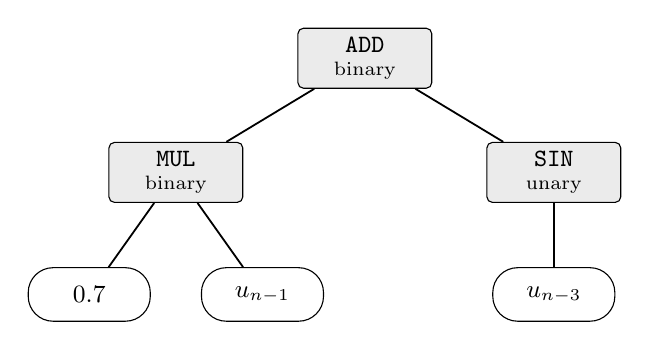
\begin{tikzpicture}[
    operator/.style={
        draw,
        rounded corners=2pt,
        fill=black!8,
        minimum width=1.7cm,
        minimum height=0.72cm,
        align=center,
        font=\small
    },
    leaf/.style={
        draw,
        rounded corners=9pt,
        fill=white,
        minimum width=1.55cm,
        minimum height=0.68cm,
        align=center,
        font=\small
    },
    branch/.style={draw, line width=0.65pt}
]
    \node[operator] (add) at (0,0)
        {\texttt{ADD}\\[-1mm]{\scriptsize binary}};
    \node[operator] (mul) at (-2.4,-1.45)
        {\texttt{MUL}\\[-1mm]{\scriptsize binary}};
    \node[operator] (sin) at (2.4,-1.45)
        {\texttt{SIN}\\[-1mm]{\scriptsize unary}};

    \node[leaf] (constant) at (-3.5,-3.0) {$0.7$};
    \node[leaf] (lagone) at (-1.3,-3.0) {$u_{n-1}$};
    \node[leaf] (lagthree) at (2.4,-3.0) {$u_{n-3}$};

    \draw[branch] (add) -- (mul);
    \draw[branch] (add) -- (sin);
    \draw[branch] (mul) -- (constant);
    \draw[branch] (mul) -- (lagone);
    \draw[branch] (sin) -- (lagthree);
\end{tikzpicture}
\caption{Example unary--binary tree for
$u_n=0.7u_{n-1}+\sin(u_{n-3})$. Binary nodes have two children, the unary
\texttt{SIN} node has one child, and the leaves contain a constant or a lagged
sequence term.}
\label{fig:dascoli-unary-binary-tree}
\end{figure}

Reading Fig.~\ref{fig:dascoli-unary-binary-tree} from the root and recursively
visiting each subtree from left to right produces the prefix representation.
The same tree is serialized in prefix, or Polish, notation, giving a target
such as
\[
    [\texttt{add},\texttt{mul},0.7,u_{n-1},
      \texttt{sin},u_{n-3}].
\]
This representation preserves tree structure without parentheses and allows
the Transformer decoder to generate the recurrence as a token sequence.

\paragraph{How a recovered formula is evaluated.}
Different syntax trees can express the same numerical mechanism. Consequently,
the paper evaluates a predicted recurrence behaviorally: it executes the
predicted and reference formulas from the same initial conditions and checks
the relative error of the next $n_{\mathrm{pred}}$ terms against a tolerance.
This avoids treating an algebraically equivalent expression as wrong merely
because its tokens differ. Beam candidates can likewise be ranked by executing
them and measuring how well they reconstruct the observed sequence.

\paragraph{Contribution to the proposed benchmark.}
This work supplies an expression-first formula sampler for the present thesis:
sample a valid abstract syntax tree, retain that tree as the auditable
mechanism, and execute it to obtain observations. The thesis can extend the
leaf vocabulary with explicit multivariate operators such as
$\operatorname{LAG}(j,\ell)$ and extend the grammar with stochastic
innovations, regime switches, and controlled interaction nodes. Retaining the
sampled tree then supports several references from the same example: its exact
symbolic equation, variable--lag support, signed coefficients when defined,
realized local term values, and generator-based attributions. In the original
study, the tree supervises symbolic-recurrence recovery; in this benchmark, the
same retained mechanism additionally anchors explanation-ground-truth
generation and comparison with forecasting and XAI methods.


\subsubsection{HVAE for Efficient Generation of Mathematical Expressions}

In \emph{Efficient Generator of Mathematical Expressions for Symbolic
Regression}, \citet{meznar2023efficient} address the generation of candidate
equations for symbolic regression. Their central model is a hierarchical
variational autoencoder (HVAE) that represents every expression directly as a
binary tree: internal nodes contain binary operators or unary functions, while
leaves contain variables or constants. The associated EDHiE method searches
the HVAE's continuous latent space for an expression whose evaluated values
fit an observed dataset. This makes the paper relevant to the formula-sampling
stage of the proposed benchmark: a learned prior over trees can concentrate
samples around expression structures found in a selected scientific domain.

\paragraph{Where the training trees come from.}
Before HVAE can sample new expressions, it learns from a corpus of valid trees.
In the experiments, this corpus is produced with probabilistic context-free
grammars and then simplified with SymPy. One reported arithmetic grammar
recursively selects addition or subtraction, multiplication or division, and
parenthesized subexpressions, constants, or variables; a second version also
contains sine and cosine. Consequently, HVAE learns the distribution supplied
by its training corpus rather than beginning from an empty expression space.
For the present thesis, that corpus could instead contain safe discrete-time
mechanisms whose leaves are constants, the current index, and
$\operatorname{LAG}(j,\ell)$ terms.

\paragraph{How HVAE learns a distribution over trees.}
The encoder processes a tree bottom-up. At node $v$, a GRU$_{2\rightarrow1}$
cell combines the symbol stored at $v$ with the representations of its left and
right children. The final root representation is mapped to the mean and
log-variance of a Gaussian latent code. The decoder reverses this direction.
It maps a latent vector to a root state and recursively expands the tree with a
GRU$_{1\rightarrow2}$ cell whose shared parameters are reused at every node.
In the notation of this review, one decoding step is

\begin{equation}
\begin{aligned}
\mathbf z &\sim \mathcal N(\mathbf 0,\mathbf I),
&\mathbf h_{\varnothing}&=\mathbf W_z\mathbf z+\mathbf b_z,\\
\boldsymbol\pi_v
  &=\operatorname{softmax}(\mathbf W_s\mathbf h_v+\mathbf b_s),
&s_v&=\arg\max_s \pi_{v,s},\\
(\mathbf h_{vL},\mathbf h_{vR})
  &=\operatorname{GRU}_{1\rightarrow2}
    (\boldsymbol\pi_v,\mathbf h_v).&&
\end{aligned}
\label{eq:meznar-hvae-decoder}
\end{equation}

The selected symbol determines the tree structure. A binary operator activates
both child states, a unary function activates only the left child, and a
variable or constant terminates that branch. The released decoder selects the
largest softmax probability and, at the configured maximum height, restricts
the choice to leaf symbols.\footnote{Official HVAE implementation:
\url{https://github.com/smeznar/HVAE}; see the recursive decoding and
\texttt{sample\_symbol} routines in \texttt{EDHiE/model.py}.} Thus a latent
draw leads to a complete tree by the following recursion:

\begin{enumerate}
    \item sample $\mathbf z\sim\mathcal N(\mathbf 0,\mathbf I)$ and transform it
    into the root state $\mathbf h_{\varnothing}$;
    \item calculate $\boldsymbol\pi_v$ and choose symbol $s_v$ at the current
    node;
    \item if $a(s_v)=2$, create and decode the left and right child states;
    if $a(s_v)=1$, decode only the left state; if $a(s_v)=0$, close the branch;
    \item repeat the same decoder cell until every branch reaches a leaf;
    \item fit any free constants and execute the resulting expression when it
    is evaluated as a symbolic-regression candidate.
\end{enumerate}

\begin{figure}[H]
\centering
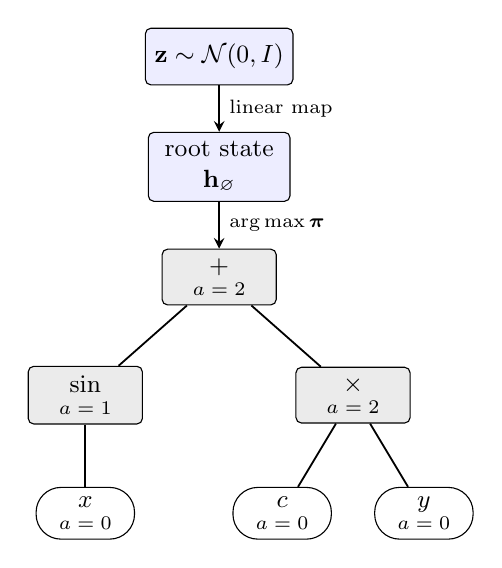
\begin{tikzpicture}[
    state/.style={
        draw,
        rounded corners=2pt,
        fill=blue!7,
        minimum width=1.8cm,
        minimum height=0.72cm,
        align=center,
        font=\small
    },
    operator/.style={
        draw,
        rounded corners=2pt,
        fill=black!8,
        minimum width=1.45cm,
        minimum height=0.68cm,
        align=center,
        font=\small
    },
    leaf/.style={
        draw,
        rounded corners=9pt,
        fill=white,
        minimum width=1.25cm,
        minimum height=0.62cm,
        align=center,
        font=\small
    },
    flow/.style={->,>=stealth,draw,line width=0.7pt},
    branch/.style={draw,line width=0.65pt}
]
    \node[state] (latent) at (0,1.8)
        {$\mathbf z\sim\mathcal N(0,I)$};
    \node[state] (rootstate) at (0,0.4)
        {root state\\$\mathbf h_{\varnothing}$};
    \node[operator] (add) at (0,-1.0)
        {$+$\\[-1mm]{\scriptsize $a=2$}};
    \node[operator] (sin) at (-1.7,-2.5)
        {$\sin$\\[-1mm]{\scriptsize $a=1$}};
    \node[operator] (mul) at (1.7,-2.5)
        {$\times$\\[-1mm]{\scriptsize $a=2$}};
    \node[leaf] (x) at (-1.7,-4.0)
        {$x$\\[-1mm]{\scriptsize $a=0$}};
    \node[leaf] (c) at (0.8,-4.0)
        {$c$\\[-1mm]{\scriptsize $a=0$}};
    \node[leaf] (y) at (2.6,-4.0)
        {$y$\\[-1mm]{\scriptsize $a=0$}};

    \draw[flow] (latent) -- node[right,font=\scriptsize]{linear map}
        (rootstate);
    \draw[flow] (rootstate) -- node[right,font=\scriptsize]{$\arg\max\boldsymbol\pi$}
        (add);
    \draw[branch] (add) -- (sin);
    \draw[branch] (add) -- (mul);
    \draw[branch] (sin) -- (x);
    \draw[branch] (mul) -- (c);
    \draw[branch] (mul) -- (y);
\end{tikzpicture}
\caption{Top-down HVAE decoding of one latent draw into the valid expression
$\sin(x)+c\,y$. Each predicted symbol determines how many descendant states
are decoded: two for a binary operator, one for a unary function, and zero for
a leaf.}
\label{fig:meznar-hvae-sampling}
\end{figure}

The standard sampling method, HVAR, repeats this process for independent
Gaussian latent draws. EDHiE searches the same space more deliberately: its
initial population is sampled from $\mathcal N(\mathbf 0,\mathbf I)$, crossover
forms convex combinations of two parent vectors, and mutation interpolates
between the encoded neighborhood of one expression and the standard Gaussian
prior. Candidate fitness is calculated only after decoding the vector, fitting
its constants, and evaluating the resulting equation on the observations
\citep{meznar2023efficient}.

\paragraph{Efficiency and relevance to the benchmark.}
The experiments report syntactically valid HVAE outputs, substantially lower
reconstruction error with 2,000 training expressions than the sequential VAE
obtains with 12,000, and effective operation in a 32-dimensional latent space.
On the Nguyen benchmark, latent-space random search reconstructs more equations
than the manually specified probabilistic-grammar baseline, while EDHiE adds an
evolutionary search over the learned space. For the proposed benchmark, HVAE
could therefore replace uniform formula sampling with a domain-shaped prior.
Its symbol library would include $\operatorname{LAG}(j,\ell)$, and each decoded
tree would pass numerical-domain, stability, variable-coverage, and recurrence
checks before it generated a time series. The retained decoded tree would then
supply the same structural, coefficient, local-contribution, gradient, and
Shapley references defined elsewhere in this thesis.


\subsubsection{Controllable Neural Symbolic Regression}

\citet{bendinelli2023controllable} introduce Neural Symbolic Regression with
Hypotheses (NSRwH). The method receives both a numerical dataset and a set of
user-supplied hypotheses about the desired equation, then generates candidate
expressions conditioned on both sources. It extends the pretrained neural
symbolic-regression pipeline of NeSymReS \citep{biggio2021neural}: synthetic
expressions are sampled and evaluated to create training pairs, while a
Transformer learns the inverse mapping from the evaluated points back to a
prefix expression. NSRwH adds explicit structural control to this inverse
mapping.

\paragraph{How the synthetic expressions and numerical data are sampled.}
Every training example is a triple $(e,\mathcal D,\mathcal H)$. The first two
elements are constructed as follows \citep{bendinelli2023controllable}.

\begin{enumerate}
    \item Sample a random unary--binary expression-tree shape using the
    procedure of Lample and Charton. The paper restricts depth to
    $1,\ldots,6$, prefix length to at most 20 tokens, and the number of input
    variables to at most five. The released configuration also sets a maximum
    of six operator insertions.

    \item Assign an operator of matching arity to every internal node. The
    reported unary library is
    \[
      \{\sqrt{\cdot},(\cdot)^2,(\cdot)^3,(\cdot)^4,
        (\cdot)^{-1},\log,\exp,\sin,\cos,\arcsin\};
    \]
    the binary library is $\{+,-,\times,\div\}$. Leaves receive variables
    $x_1,\ldots,x_5$ or constant placeholders.

    \item Simplify the expression with SymPy. Sample additive constants
    uniformly on $[-10,10]$ and positive multiplicative constants
    log-uniformly on $[0.05,10]$.

    \item For each active variable, sample the two limits of its support from
    $[-10,10]$, requiring an interval width of at least one. Then sample
    $n\in\{1,\ldots,1000\}$ input points independently within those limits.

    \item Evaluate $e$ at the sampled points to obtain
    $\mathcal D=\{(\mathbf x_i,e(\mathbf x_i))\}_{i=1}^{n}$. Inputs producing
    NaNs or magnitudes above the half-precision limit 65504 are discarded and
    resampled.
\end{enumerate}

The official generator makes the first step more precise. It precomputes the
number of unary--binary trees that can complete each combination of open leaf
positions and remaining operators. At each iteration it uses these counts to
sample (i) which still-empty position receives the next operator and (ii)
whether that operator is unary or binary. It then samples the concrete operator
from configurable weights, opens the required child positions, and eventually
fills all remaining positions with variables. This produces a complete prefix
tree with a controlled operator budget rather than growing branches until an
uncontrolled stopping event.\footnote{Official NSRwH implementation:
\href{https://github.com/SymposiumOrganization/ControllableNeuralSymbolicRegression}
{official NSRwH repository}; see \texttt{dataset/generator.py} and
\texttt{configs/dataset\_configuration.json}.}

\paragraph{How the hypotheses are generated.}
During pretraining, $\mathcal H$ is extracted from the known sampled expression
$e$. At inference, the same fields can be supplied by a scientist as complete,
partial, or uncertain prior knowledge.

\begin{table}[tbp]
\centering
\small
\renewcommand{\arraystretch}{1.08}
\begin{tabular}{@{}p{0.22\textwidth}p{0.70\textwidth}@{}}
\toprule
Hypothesis & Information encoded for the expression decoder \\
\midrule
Complexity & Number of operators, variables, and constants in the expression. \\
Symmetry & Tokens indicating whether selected groups of input variables have
generalized symmetry. \\
Positive branches & Prefix subtrees known to occur in $e$. The complete tree
and trivial one-variable branches are excluded. \\
Negative branches & Prefix subtrees selected from the training distribution
and known to be absent from $e$. \\
Known constants & Numerical constant values paired with pointer tokens that
identify where the decoder may place them. \\
\bottomrule
\end{tabular}
\caption{The five hypothesis families used to condition NSRwH.}
\label{tab:nsrwh-hypotheses}
\end{table}

Positive and negative candidate subtrees are enumerated with depth-first
search. A subtree of prefix length $L_s$ is sampled with weight proportional
to $L_s^{-2}$, so short fragments are presented more often. Parameters
$p_{+}$ and $p_{-}$ control the total number of positive and negative tokens:
sampling continues until their aggregate lengths reach approximately
$p_{+}|e|$ and $p_{-}|e|$, respectively. Masking different hypothesis families
during training teaches one model to operate with many levels of available
prior information.

\paragraph{Architecture and controlled expression decoding.}
NSRwH contains a numerical set encoder, a symbolic hypothesis encoder, and an
autoregressive Transformer decoder. Numerical values first receive a 16-bit
multi-hot representation and an embedding. A set Transformer maps the
unordered input--output points to $\mathbf z_{\mathrm{num}}$. A second set
Transformer maps the hypothesis tokens to $\mathbf z_{\mathrm{hyp}}$. Both
outputs have compatible shape and are combined elementwise:

\begin{equation}
\begin{aligned}
\mathbf z_{\mathrm{num}}&=\operatorname{Enc}_{\mathrm{num}}(\mathcal D),\\
\mathbf z_{\mathrm{hyp}}&=\operatorname{Enc}_{\mathrm{hyp}}(\mathcal H),\\
\mathbf z_{\mathrm{fuse}}&=
    \mathbf z_{\mathrm{num}}+\mathbf z_{\mathrm{hyp}},\\
p_{\phi}(e\mid\mathcal D,\mathcal H)
    &=\operatorname{Dec}_{\phi}(\mathbf z_{\mathrm{fuse}}).
\end{aligned}
\label{eq:nsrwh-fusion}
\end{equation}

The decoder predicts the prefix expression token by token and uses beam search
to retain several candidates. Equation~\eqref{eq:nsrwh-fusion} is the source of
controllability: changing $\mathcal H$ changes the decoder distribution without
retraining the network. Known numerical constants use pointer tokens, avoiding
one vocabulary entry for every possible real number. Remaining constants are
fitted with BFGS, after which candidates are ranked by their numerical fit.

The reported model was trained on 200 million expressions using three NVIDIA
RTX 3090 GPUs for five days with batch size 400. The numerical encoder and
expression decoder each use five layers; the hidden dimension is 512. Training
uses teacher-forced next-token cross-entropy, while inference uses beam search.
The paper separates three evaluation questions: \emph{is satisfied} measures
how often decoded expressions obey the supplied hypothesis; \emph{is correct}
requires numerical agreement at more than 99\% of held-out support points; and
mean $R^2$ measures numerical fit. This distinction prevents an expression that
obeys the requested structure but predicts poorly from being counted as a
successful mechanism recovery.

\begin{figure}[H]
\centering
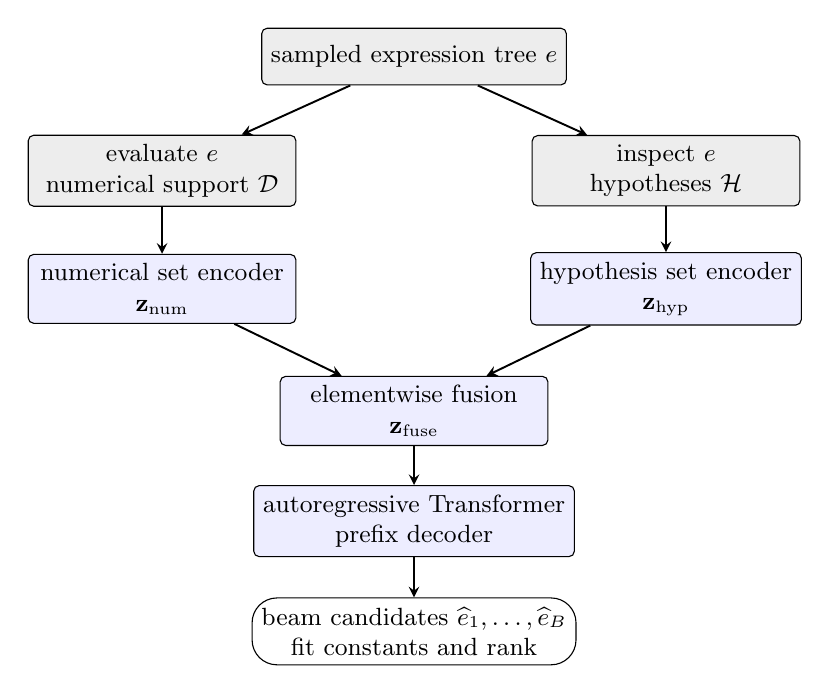
\begin{tikzpicture}[
    block/.style={
        draw,
        rounded corners=2pt,
        fill=blue!7,
        minimum width=3.4cm,
        minimum height=0.72cm,
        align=center,
        font=\small
    },
    source/.style={
        draw,
        rounded corners=2pt,
        fill=black!7,
        minimum width=3.4cm,
        minimum height=0.72cm,
        align=center,
        font=\small
    },
    output/.style={
        draw,
        rounded corners=9pt,
        fill=white,
        minimum width=4.0cm,
        minimum height=0.68cm,
        align=center,
        font=\small
    },
    flow/.style={->,>=stealth,draw,line width=0.7pt}
]
    \node[source] (tree) at (0,3.2)
        {sampled expression tree $e$};
    \node[source] (data) at (-3.2,1.75)
        {evaluate $e$\\numerical support $\mathcal D$};
    \node[source] (hyp) at (3.2,1.75)
        {inspect $e$\\hypotheses $\mathcal H$};
    \node[block] (numenc) at (-3.2,0.25)
        {numerical set encoder\\$\mathbf z_{\mathrm{num}}$};
    \node[block] (hypenc) at (3.2,0.25)
        {hypothesis set encoder\\$\mathbf z_{\mathrm{hyp}}$};
    \node[block] (fuse) at (0,-1.3)
        {elementwise fusion\\$\mathbf z_{\mathrm{fuse}}$};
    \node[block] (decoder) at (0,-2.7)
        {autoregressive Transformer\\prefix decoder};
    \node[output] (candidates) at (0,-4.1)
        {beam candidates $\widehat e_1,\ldots,\widehat e_B$\\
         fit constants and rank};

    \draw[flow] (tree) -- (data);
    \draw[flow] (tree) -- (hyp);
    \draw[flow] (data) -- (numenc);
    \draw[flow] (hyp) -- (hypenc);
    \draw[flow] (numenc) -- (fuse);
    \draw[flow] (hypenc) -- (fuse);
    \draw[flow] (fuse) -- (decoder);
    \draw[flow] (decoder) -- (candidates);
\end{tikzpicture}
\caption{NSRwH training pipeline. The same sampled tree supplies the numerical
observations and the structurally correct hypothesis tokens. At inference, the
two encoder inputs steer a shared prefix-expression decoder.}
\label{fig:nsrwh-pipeline}
\end{figure}

\paragraph{Contribution to the proposed benchmark.}
NSRwH provides a design for controlled mechanism retrieval. The benchmark can
derive $\mathcal H$ automatically from every retained generator tree, then
evaluate recovery under complete, partial, deliberately missing, or partially
incorrect hypotheses. For time series, positive and negative branches can
encode required or forbidden variable--lag subtrees, complexity can control
mechanism size, known constants can expose selected coefficients, and symmetry
can describe exchangeable source variables. The generator remains responsible
for structural, signed, local-contribution, gradient, and Shapley ground truth;
NSRwH supplies a controlled symbolic model whose recovered tree can be compared
with that ground truth.


\subsubsection{ODEFormer: symbolic regression of continuous-time dynamics}

\citet{dascoli2024odeformer} study \emph{dynamical symbolic regression}. The
observations are samples of one continuous-time trajectory,
$\{(t_i,\mathbf x_i)\}_{i=1}^{N}$, and the symbolic target is the vector field
that governs its instantaneous evolution:

\begin{equation}
\dot{\mathbf x}(t)=\mathbf f(\mathbf x(t)),
\qquad
\mathbf f=(f_1,\ldots,f_{D_{\mathrm{ode}}}):
\mathbb R^{D_{\mathrm{ode}}}\rightarrow
\mathbb R^{D_{\mathrm{ode}}}.
\label{eq:odeformer-vector-field}
\end{equation}

This extends the expression-first principle used by D'Ascoli et al.: first
sample a symbolic mechanism and then execute it to generate observations. The
tree representation remains unary--binary and the target remains a prefix
token sequence. The important change is the meaning of execution. A recurrence
tree directly calculates the next discrete sample; an ODE tree calculates
$\dot{\mathbf x}$ at the current state, and a numerical solver repeatedly
evaluates that tree to produce the observed trajectory.

\paragraph{Sampling a symbolic ODE system.}
The system dimension is sampled uniformly up to
$D_{\mathrm{ode}}=6$. One expression tree is generated independently for each
component $f_k$. For every component, ODEFormer performs the following steps
\citep{dascoli2024odeformer}:

\begin{enumerate}
    \item sample between one and five binary operators and construct a random
    binary-tree shape using the same completion-count procedure used in
    Transformer symbolic-regression generators;

    \item assign addition with probability $3/4$ or multiplication with
    probability $1/4$ to each binary node, and assign a state variable
    $x_j$, $j\in\{1,\ldots,D_{\mathrm{ode}}\}$, to each leaf;

    \item sample between zero and three unary insertions. Each insertion places
    one of $\sin(\cdot)$, $(\cdot)^{-1}$, or $(\cdot)^2$ above a selected
    subtree whose depth remains below six;

    \item add signed coefficients to terms and affine transformations inside
    unary arguments. Their absolute values are sampled log-uniformly between
    $0.05$ and $20$;

    \item serialize $f_1,\ldots,f_{D_{\mathrm{ode}}}$ in prefix notation and
    separate consecutive component equations with a dedicated token
    $\texttt{|}$.
\end{enumerate}

Subtraction is represented by addition with a negative coefficient, while
division is represented by multiplication with an inverse. For example, the
tree

\begin{equation}
f_1(\mathbf x)=a x_1+\sin(bx_2)
\quad\longleftrightarrow\quad
[\texttt{add},\texttt{mul},a,x_1,
  \texttt{sin},\texttt{mul},b,x_2]
\label{eq:odeformer-prefix-example}
\end{equation}

uses exactly the same symbolic objects as functional or recurrent symbolic
regression. Its meaning is now $\dot x_1=f_1(\mathbf x)$.

\begin{figure}[H]
\centering
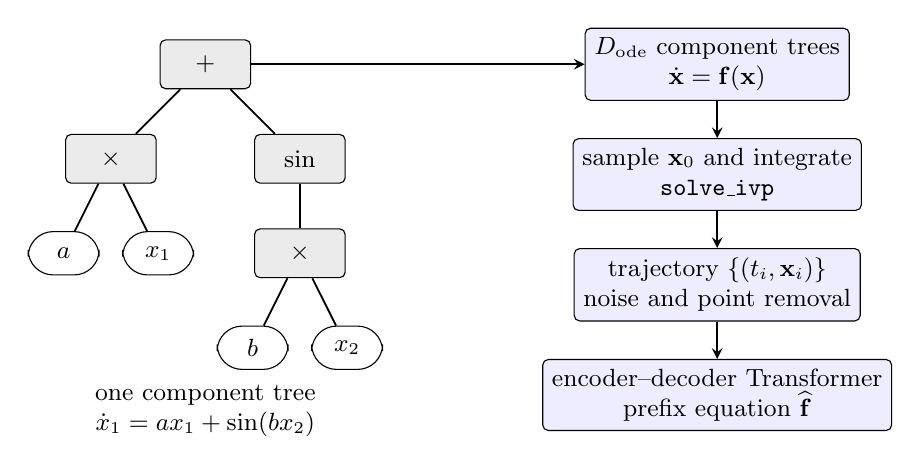
\begin{tikzpicture}[
    operator/.style={draw,rounded corners=2pt,fill=black!8,
        minimum width=1.15cm,minimum height=0.62cm,align=center,font=\small},
    leaf/.style={draw,rounded corners=9pt,fill=white,
        minimum width=0.90cm,minimum height=0.55cm,align=center,font=\small},
    block/.style={draw,rounded corners=2pt,fill=blue!7,
        minimum width=3.15cm,minimum height=0.70cm,align=center,font=\small},
    flow/.style={->,>=stealth,draw,line width=0.7pt},
    branch/.style={draw,line width=0.65pt}
]
    \node[operator] (add) at (-4.4,2.4) {$+$};
    \node[operator] (mul1) at (-5.6,1.2) {$\times$};
    \node[operator] (sin) at (-3.2,1.2) {$\sin$};
    \node[leaf] (a) at (-6.2,0.0) {$a$};
    \node[leaf] (x1) at (-5.0,0.0) {$x_1$};
    \node[operator] (mul2) at (-3.2,0.0) {$\times$};
    \node[leaf] (b) at (-3.8,-1.2) {$b$};
    \node[leaf] (x2) at (-2.6,-1.2) {$x_2$};
    \draw[branch] (add)--(mul1); \draw[branch] (add)--(sin);
    \draw[branch] (mul1)--(a); \draw[branch] (mul1)--(x1);
    \draw[branch] (sin)--(mul2);
    \draw[branch] (mul2)--(b); \draw[branch] (mul2)--(x2);
    \node[font=\small,align=center] at (-4.4,-2.0)
        {one component tree\\$\dot x_1=a x_1+\sin(bx_2)$};

    \node[block] (trees) at (2.1,2.4)
        {$D_{\mathrm{ode}}$ component trees\\$\dot{\mathbf x}=\mathbf f(\mathbf x)$};
    \node[block] (integrate) at (2.1,1.0)
        {sample $\mathbf x_0$ and integrate\\\texttt{solve\_ivp}};
    \node[block] (trajectory) at (2.1,-0.4)
        {trajectory $\{(t_i,\mathbf x_i)\}$\\noise and point removal};
    \node[block] (transformer) at (2.1,-1.8)
        {encoder--decoder Transformer\\prefix equation $\widehat{\mathbf f}$};
    \draw[flow] (add.east) -- (trees.west);
    \draw[flow] (trees)--(integrate);
    \draw[flow] (integrate)--(trajectory);
    \draw[flow] (trajectory)--(transformer);
\end{tikzpicture}
\caption{What remains and what changes in ODEFormer. The symbolic mechanism is
still a unary--binary tree. Numerical integration is inserted between that
tree and the observations because the tree specifies a derivative rather than
the next sample directly.}
\label{fig:odeformer-tree-pipeline}
\end{figure}

\paragraph{From an equation to a training trajectory.}
After sampling $\mathbf f$, the generator draws
$\mathbf x_0\sim\mathcal N(\mathbf 0,\mathbf I)$ and integrates
Equation~\eqref{eq:odeformer-vector-field} from $t=1$ to $t=10$. The number of
stored points $N$ is sampled uniformly from 50 to 200. The implementation uses
SciPy's \texttt{solve\_ivp}, whose default method is adaptive RK45. Failed
integrations and trajectories with $|x_j|>10^2$ are discarded. When every
component becomes nearly constant during the final quarter of the interval,
the example is discarded with probability $0.9$ so that fixed-point solutions
do not dominate the training distribution.

Two corruptions make the observations resemble measurements. A noise scale
$\sigma\sim\mathcal U(0,0.1)$ produces multiplicative Gaussian noise,

\begin{equation}
x_j(t_i)\leftarrow(1+\xi_{i,j})x_j(t_i),
\qquad \xi_{i,j}\sim\mathcal N(0,\sigma^2),
\label{eq:odeformer-noise}
\end{equation}

and a sampled ratio $\rho\sim\mathcal U(0,0.5)$ removes that fraction of time
points uniformly. Consequently, a training pair contains a noisy, irregularly
sampled trajectory as input and the exact prefix representation of the sampled
vector field as target. The formula is retained before integration, so it is
available as mechanism ground truth.

\paragraph{Architecture and inference.}
ODEFormer uses an encoder--decoder Transformer with 86 million parameters, 16
attention heads, and embedding dimension 512. The encoder has four layers and
the decoder has 16. Each timestamp and state value is rounded to four
significant digits and represented by three tokens: sign, mantissa, and
exponent. A feed-forward embedder combines the tokens belonging to one observed
point. Since time is included explicitly in every point, the numerical encoder
uses the timestamps instead of positional embeddings.

The decoder generates the component equations autoregressively in prefix
notation. Beam sampling produces candidate systems; the reported default uses
beam size 50 and temperature 0.1. Every candidate is integrated from the
observed initial condition, and the equation with the highest reconstruction
$R^2$ is selected. An optional BFGS step refines numerical constants. The
complete implementation is released by the authors.\footnote{Official
ODEFormer implementation: \url{https://github.com/sdascoli/odeformer}.}

\paragraph{How mechanism recovery is evaluated.}
The paper distinguishes two trajectory-level tests:

\begin{itemize}
    \item \emph{reconstruction}: integrate $\widehat{\mathbf f}$ from the same
    initial condition and over the same interval used to produce the observed
    trajectory;
    \item \emph{generalization}: integrate $\mathbf f$ and
    $\widehat{\mathbf f}$ from a new initial condition, then compare their
    trajectories over the same time interval.
\end{itemize}

The principal accuracy statistic is the percentage of systems for which the
trajectory $R^2$ exceeds $0.9$. The authors additionally report expression
complexity, defined as the total number of operators, variables, and constants,
and inference time. Generalization is the stronger mechanism-recovery test: two
equations may follow one observed path while generating different dynamics in
other parts of the state space. This also explains why recovering an ODE from
one trajectory is an identifiability problem rather than only a forecasting
problem.

\paragraph{What the recovered ODE explains.}
An explicit ODE gives a global, mechanistic description of the instantaneous
dynamics. For example, the occurrence of $x_j$ in $f_k$ states that variable
$j$ directly participates in the rate of change of variable $k$. This yields a
structural reference

\begin{equation}
M^{\mathrm{GT,ODE}}_{k,j}
=\mathbb I[x_j\text{ occurs in the sampled tree for }f_k].
\label{eq:odeformer-structural-gt}
\end{equation}

A local derivative-level influence can also be calculated from the Jacobian,

\begin{equation}
J_{k,j}(t)=
\left.\frac{\partial f_k(\mathbf x)}{\partial x_j}
\right|_{\mathbf x=\mathbf x(t)}.
\label{eq:odeformer-jacobian}
\end{equation}

These quantities explain which variables govern the \emph{instantaneous rate
of change}. Explaining a finite-horizon state
$\Phi_{\mathbf f}(\Delta;\mathbf x_0)$ requires propagating influence through
the integration. One principled reference is the flow sensitivity

\begin{equation}
\mathbf S(\Delta)=
\frac{\partial\Phi_{\mathbf f}(\Delta;\mathbf x_0)}{\partial\mathbf x_0},
\qquad
\dot{\mathbf S}(t)=
\mathbf J_{\mathbf f}(\mathbf x(t))\mathbf S(t),
\quad \mathbf S(0)=\mathbf I.
\label{eq:odeformer-flow-sensitivity}
\end{equation}

Equations~\eqref{eq:odeformer-structural-gt}--
\eqref{eq:odeformer-flow-sensitivity} are a benchmark interpretation proposed
for this thesis. ODEFormer evaluates reconstructed and generalized trajectories
instead. The distinction resolves the apparent loss of explainability: the
symbolic ODE makes the governing law explicit, while a contribution to a
particular future state additionally depends on the initial condition, the
visited trajectory, interactions, and the chosen horizon.

\paragraph{Position in the proposed research.}
ODEFormer provides a useful advanced extension and a methodological bridge to
continuous-time system identification. The November benchmark can keep its
core around discrete-time recurrences, where a sampled tree directly generates
the next observation and all variable--lag references are immediate. A later
continuous-time module can reuse the same expression-tree interface while
adding initial-condition sampling, numerical integration, solver-failure
filters, and flow-based explanation references. This staging preserves the
main software design while separating the additional numerical and
identifiability challenges of ODE discovery.


\paragraph{Differences among the four approaches in Section~1.2.}
D'Ascoli et al. directly sample a discrete lagged recurrence, execute it to
produce a sequence, and train a Transformer to recover the recurrence from that
sequence. Me\v{z}nar et al. learn an unconditional continuous prior over general
expression trees and search that latent space for equations fitting numerical
data. Bendinelli et al. retain an explicit random-tree prior for pretraining and
learn the conditional inverse map
$p_{\phi}(e\mid\mathcal D,\mathcal H)$, allowing hypotheses to steer which
equation is recovered. NSRwH is therefore a direct extension of the NeSymReS
family and contributes controlled recovery; D'Ascoli's construction supplies
the discrete temporal-generator role. ODEFormer retains random unary--binary
trees and prefix decoding, but interprets each tree as one component of a
continuous-time vector field and uses numerical integration to connect the
equation with observations. For this thesis, the four contributions compose
naturally: D'Ascoli supplies the lagged grammar and executable recurrence, HVAE
offers an optional learned prior over plausible recurrence trees, NSRwH supplies
a retriever that can be tested with different amounts and qualities of known
mechanism information, and ODEFormer supplies the continuous-time extension in
which evaluation must include trajectory reconstruction and generalization.



\subsection{Synthetic Priors for Time-Series Foundation Models}

This subsection examines a second use of synthetic time series: constructing a
large pretraining distribution for a forecasting foundation model. The central
object in these works is a \emph{prior over possible series}. Sampling many
independent mechanisms and trajectories exposes one model to a wider range of
trends, seasonalities, correlations, regime changes, and noise processes than
is available in a single real dataset. This objective complements the
explanation benchmarks in Section~1.1: the same generator can provide training
diversity, while a benchmark additionally retains the sampled mechanism and
derives an explicit reference explanation from it.

\subsubsection{KernelSynth and its role in Chronos-2}

\paragraph{Provenance and role.}
KernelSynth was introduced with the original Chronos model by
\citet{ansari2024chronos}. Chronos-2 subsequently uses KernelSynth as one of
four base univariate generators---AR, ETS, TSI, and KernelSynth---before
imposing multivariate structure through additional transformations
\citep{ansari2025chronos2}. Thus, KernelSynth supplies elementary stochastic
trajectories; the Chronos-2 data pipeline supplies the cross-series structure
needed for multivariate and covariate-informed tasks.

\paragraph{How KernelSynth generates one series.}
KernelSynth reverses the compositional-kernel-search idea. Instead of observing
a series and searching for a Gaussian-process kernel that describes it, the
method first samples a composite kernel and then draws a function from the
corresponding Gaussian-process prior. Let $\mathcal K$ be the kernel bank and
let $J_K=5$ be the maximum number of kernels in one composition. The procedure
is

\begin{equation}
\begin{aligned}
R_K &\sim \mathcal U\{1,\ldots,J_K\},\\
\kappa_1,\ldots,\kappa_{R_K}
    &\overset{\mathrm{i.i.d.}}{\sim}\mathcal K,\\
\kappa_\star
    &=(((\kappa_1\circ_2\kappa_2)\circ_3\kappa_3)\cdots)
      \circ_{R_K}\kappa_{R_K},
      \qquad \circ_r\sim\mathcal U\{+,\times\},\\
x_{1:T_{\mathrm{syn}}}
    &\sim \operatorname{GP}(0,\kappa_\star),
    \qquad T_{\mathrm{syn}}=1024.
\end{aligned}
\label{eq:kernelsynth}
\end{equation}

The final line means that the implementation evaluates $\kappa_\star$ on
$T_{\mathrm{syn}}$ evenly spaced points between zero and one to obtain a
covariance matrix $\mathbf K_\star$, then samples the complete vector
$\mathbf x\sim\mathcal N(\mathbf 0,\mathbf K_\star)$. Every draw is therefore
a different trajectory even when the same composite kernel is reused. The
kernel bank in the paper and released implementation is summarized in
Table~\ref{tab:kernelsynth-bank}.

\begin{table}[H]
\centering
\small
\renewcommand{\arraystretch}{1.08}
\begin{tabular}{@{}p{0.19\textwidth}p{0.36\textwidth}p{0.36\textwidth}@{}}
\toprule
Kernel family & Temporal behavior represented & Values used in the bank \\
\midrule
Constant & Shared level covariance & $C=1$ \\
White noise & Independent short-scale variation & noise level $0.1$ or $1$ \\
Linear & Globally varying trend-like functions & offset scale $0$, $1$, or $10$ \\
RBF & Smooth local variation & length scale $0.1$, $1$, or $10$ \\
Rational quadratic & Variation over a mixture of length scales &
shape $0.1$, $1$, or $10$ \\
Periodic & Repeating patterns over common temporal frequencies &
hourly-, daily-, weekly-, monthly-, quarterly-, and yearly-inspired periods \\
\bottomrule
\end{tabular}
\caption{Basis-kernel families used by KernelSynth. The released code stores
several parameterized instances of each family in $\mathcal K$, so sampling is
over kernel type and parameterization.}
\label{tab:kernelsynth-bank}
\end{table}

The released bank contains 33 parameterized entries. Kernels are sampled with
replacement, their periodicities are normalized by $T_{\mathrm{syn}}$, and the
sampled sequence is reduced from left to right. Table~\ref{tab:kernelsynth-bank}
summarizes the families rather than reproducing every entry. If numerical GP
sampling fails, the public script discards that attempt and samples again.
Its Arrow record stores only the arbitrary start timestamp and the generated
target; the sampled kernel expression is available during generation but is
not retained in the released record.\footnote{Official KernelSynth generator:
\url{https://github.com/amazon-science/chronos-forecasting/blob/main/scripts/kernel-synth.py}.}

Kernel addition and multiplication have distinct meanings. If
$\kappa_\star=\kappa_a+\kappa_b$, a GP draw can be interpreted as the sum of
independent functions with the two covariance structures. A linear-plus-
periodic composition can consequently express trend-like and seasonal
variation together. If
$\kappa_\star=\kappa_a\kappa_b$, the covariance entries are multiplied
pointwise before the trajectory is sampled. An RBF-times-periodic
composition produces locally periodic behavior whose
correlation weakens with temporal distance. Repeated random compositions
therefore create a broad stochastic prior from a small kernel vocabulary.

\paragraph{How Chronos-2 constructs multivariate training tasks.}
Chronos-2 uses separate synthetic mechanisms at two levels
\citep{ansari2025chronos2}. Its univariate corpus is enlarged with TSI, which
randomly combines trend, seasonality, and irregularity components, and TCM,
which samples temporal causal graphs and generates series autoregressively.
For multivariate and covariate-informed pretraining, the data are synthetic.
A \emph{multivariatizer} first samples several base series from AR, ETS, TSI,
or KernelSynth and then introduces one of two dependency classes:

\begin{itemize}
    \item a contemporaneous multivariatizer jointly transforms several series,
    linearly or nonlinearly, at each time step. This creates instantaneous
    cross-series dependence;
    \item a sequential multivariatizer introduces dependence across different
    time steps, including lead--lag effects and cointegration-like behavior.
\end{itemize}

The resulting channels are used either as joint targets or are divided into
targets, past-only covariates, and known-future covariates. This construction
is important for interpreting the phrase ``KernelSynth in Chronos-2'':
KernelSynth creates a base univariate GP draw, while the multivariatizer is the
stage that creates the multivariate forecasting problem. The Chronos-2 paper
specifies these two classes and their purpose; the exact sampled transformation
families and parameter distributions remain outside the report's description.

\paragraph{Generation implementation and computational scaling.}
The official Chronos KernelSynth script exposes the generation as an
embarrassingly parallel offline job. Independent series are dispatched over
all available CPU workers with \texttt{joblib.Parallel}, configured with
\texttt{n\_jobs=-1}, and the
result is written to an Apache Arrow file with LZ4 compression. A composite
kernel is evaluated as a dense $T_{\mathrm{syn}}\times T_{\mathrm{syn}}$
covariance matrix. Exact GP sampling therefore retains cubic factorization
cost in $T_{\mathrm{syn}}$ and quadratic memory, while process-level parallelism
raises corpus throughput by generating different series concurrently. The
released script also defines an eigendecomposition-based sampling alternative;
its main generation path uses scikit-learn's GP sampler. This implementation
detail matters for the proposed benchmark: GP examples can be generated in
parallel, but long trajectories require either bounded length, approximate GP
sampling, structured kernels, or a different procedural generator. The public
script also does not assign stable mechanism and trajectory identifiers or a
derived seed to each record. A benchmark adaptation must add these fields so
that the same corpus is produced independently of worker scheduling.

\paragraph{Architecture that consumes the synthetic corpus efficiently.}
Chronos-2 is a 120M-parameter encoder-only Transformer derived from the T5
encoder \citep{ansari2025chronos2}. Each target or covariate dimension is
standardized from its observed context and transformed with $\operatorname{asinh}$
to compress extreme values while preserving sign. The normalized values, a
relative-time feature, and an observed/missing mask are divided into
non-overlapping patches of length $P_{\mathrm{patch}}$ and mapped by a residual
network into $D_{\mathrm{model}}$-dimensional tokens. The Transformer then
alternates:

\begin{enumerate}
    \item \emph{time attention}, which attends across patches belonging to the
    same series and uses rotary positional embeddings; and
    \item \emph{group attention}, which attends across related series at the
    same patch index, using group IDs to isolate independent forecasting tasks.
\end{enumerate}

A residual quantile head maps all requested future-patch embeddings directly
to 21 quantiles for every target and forecast step. Direct multi-patch output
avoids token-by-token trajectory sampling. Training first uses contexts up to
2048 observations and then extends them to 8192 while increasing the number of
output patches. The report measures approximately 300 series per second on one
NVIDIA A10G for a batch of 1024 series with context 2048 and horizon 64. These
designs make the \emph{forecasting model} efficient; CPU-parallel GP sampling
is the separate mechanism that constructs the original KernelSynth corpus.

\paragraph{Explanation information available from KernelSynth.}
If it is retained, the sampled composite kernel $\kappa_\star$ is an exact
record of the stochastic mechanism. For an observed context $\mathbf x_C$,
the GP conditional-mean forecast at horizon $h$ follows the Gaussian
conditioning formula \citep[Section~2.2, Eq.~(2.23)]{rasmussen2006gpml}.
Writing its extension to singular covariances with a pseudoinverse gives

\begin{equation}
g_h(\mathbf x_C;\kappa_\star)
=\mu_{h\mid C}
=\mathbf k_{hC}
  (\mathbf K_{CC}+\sigma_n^2\mathbf I)^\dagger\mathbf x_C,
\label{eq:gp-conditional-mean}
\end{equation}

so its exact input gradient is the horizon-specific row vector

\begin{equation}
\nabla_{\mathbf x_C}g_h
=\mathbf k_{hC}
 (\mathbf K_{CC}+\sigma_n^2\mathbf I)^\dagger.
\label{eq:gp-gradient}
\end{equation}

Equations~\eqref{eq:gp-conditional-mean}--\eqref{eq:gp-gradient} show how a
KernelSynth variant could enter this thesis as a dense stochastic benchmark:
the kernel composition is the mechanism ground truth, while the conditional
mean supplies an executable forecasting function and an exact gradient
reference. Here $\sigma_n^2$ denotes optional observation noise and is omitted
when the selected kernel already represents the intended noise. The
formula uses the ordinary inverse for a positive-definite observed
covariance. For a singular covariance, as with a constant kernel, the
pseudoinverse defines the conditional mean on the support of the observed
GP. An added numerical jitter changes that covariance and must be recorded.
In the singular case, the displayed row is the derivative of the stated
linear extension; data-supported perturbations stay on the GP support.
This
horizon-specific explanation is a construction proposed for the benchmark,
rather than an explanation artifact distributed with KernelSynth. Fixing
$\kappa_\star$ and resampling the GP creates several trajectories from one
mechanism; storing separate mechanism and trajectory seeds makes this operation
reproducible. Since kernel sums and products admit equivalent expressions,
mechanism recovery should compare a recorded expression or the resulting
covariance, rather than only the original expression string. The future GP
draw additionally contains conditional stochastic variation, which belongs to
irreducible forecast uncertainty rather than to a deterministic input
contribution.


\subsubsection{TempoPFN synthetic prior used by Toto 2.0}

\paragraph{Terminological distinction.}
Two similarly named works must be separated. \emph{TempoPFN}, by
\citet{moroshan2025tempopfn}, is the synthetic-data method cited and used by
Toto 2.0 \citep{khwaja2026toto2}. \emph{TimePFN}, by
\citet{taga2025timepfn}, is a different multivariate forecasting model based on
LMC-Synth; it is analyzed in the next subsection. Toto 2.0 consumes data from
the TempoPFN prior, rather than the TimePFN/LMC-Synth corpus.

\paragraph{How the TempoPFN prior generates series.}
TempoPFN defines a portfolio of complementary generator families rather than
one equation family \citep{moroshan2025tempopfn}. Adapted generators include
ForecastPFN component compositions, KernelSynth, a broader GP prior, and
CauKer structural causal models. New procedural families add sawtooth waves,
piecewise-constant steps, anomaly and spike processes, configurable sine
mixtures, and audio-inspired stochastic rhythms, financial volatility,
network traffic, and multiscale fractal signals. Its most structured stochastic
generator is a regime-switching, time-inhomogeneous Ornstein--Uhlenbeck process,

\begin{equation}
 d y_t
 =\theta(t,r_t)\bigl(\mu(t,r_t)-y_t\bigr)\,dt
  +\sigma(t,r_t)\,dW_t,
\label{eq:tempopfn-ou}
\end{equation}

where the latent regime $r_t\in\{0,1\}$ follows a Markov chain. The mean-
reversion speed, time-varying mean, and volatility can change between regimes
and evolve through polynomial, sinusoidal, logistic, or piecewise-linear
trends. Seasonal effects can modify the mean and volatility, and fractional
Brownian motion can replace $W_t$ to introduce long memory.

After a base trajectory is generated, an offline augmentation cascade expands
the prior. It optionally normalizes the source, applies an early convex
TS-Mixup, samples transformations from invariance, structure, seasonality,
signal-processing, discrete-effect, and measurement-artifact categories,
optionally applies random 1D convolution filters, performs a late TS-Mixup,
and finishes with scaling and low-amplitude noise. Examples include time
reversal, sign inversion, change points, shocks with exponential recovery,
calendar effects, amplitude modulation, differentiation or integration,
censoring, quantization, and resampling artifacts. An online stage injects
missing-value patterns. Consequently, one stored trajectory may combine a
sampled base mechanism with several independently recorded transformations.

\paragraph{High-throughput data construction.}
TempoPFN reports a corpus of approximately 10 million series with lengths up to
2048. Most procedural generators run on CPU, while neural generators such as
CauKer use a GPU. On the authors' dual 32-core AMD EPYC system, throughput for
length-2048 series ranges from $0.32$ series/s for exact KernelSynth and $0.66$
for CauKer to more than $100$ series/s for step, sine, anomaly, spike, and
sawtooth generators. This heterogeneous architecture is deliberate: expensive
GP/causal priors contribute structural richness, while inexpensive procedural
priors supply volume. During training, the loader samples a total length from
$\{128,256,512,1024,1536,2048\}$, favors length 2048, shortens by cutting or
subsampling, and then samples a history--future split. Mixed batches therefore
cover several mechanisms, context lengths, and forecast horizons.

\paragraph{How Toto 2.0 uses this prior.}
The Toto 2.0 report states that its base models are pretrained on 42.5\%
Datadog observability data and 57.5\% TempoPFN synthetic data
\citep{khwaja2026toto2}. The three larger models see 5.04 trillion points, of
which 2.90 trillion are synthetic; the 4M- and 22M-parameter models see 3.40
trillion points with the same proportions. The report identifies the
TempoPFN method and its coverage of nonstationary trends, abrupt change points,
and long-range dependencies. It reports the final mixture rather than an
itemized count for each TempoPFN generator inside the Toto corpus.

Toto 2.0 uses a decoder-only patched Transformer with patch size
$P_{\mathrm{patch}}=32$. Transformer blocks alternate causal attention along
time with full attention across variates. Contiguous patch masking replaces
autoregressive patch generation: during training, the model reconstructs
random contiguous masked spans; during inference, mask tokens occupy the
complete future horizon and the Transformer predicts that horizon in one
forward pass. A block-decoding mode remains available for very long horizons.
The output head predicts nine quantiles and is trained with pinball loss.

Three engineering choices support large-scale training. First, robust causal
$\operatorname{asinh}$ normalization controls the extreme scales and spikes
found in observability metrics. Second, NorMuon optimizes internal matrix
parameters while AdamW handles projections, biases, and normalization
parameters. Third, unit-scaled maximal-update parametrization (u-$\mu$P) lets
the authors tune a 10M-parameter proxy and transfer its learning configuration
to 4M, 22M, 313M, 1B, and 2.5B variants. Their released
\texttt{dd\_unit\_scaling} layer preserves this parametrization through
\texttt{torch.compile}, FSDP2 sharding, and data/tensor parallelism. All model
sizes train with 4096-step contexts, 32 variates per sample, and global batch
size 64. The generator portfolio provides data diversity; patch masking,
alternating attention, u-$\mu$P, and distributed sharding provide model-
training scale.

\paragraph{Explanation information available from the TempoPFN pipeline.}
The generator identity, sampled parameters, regime path, and augmentation
sequence can form a hierarchical mechanism record. For example,
Eq.~\eqref{eq:tempopfn-ou} supplies regime- and time-dependent drift and
diffusion parameters, while a step generator supplies exact change-point
locations. Their current use in Toto 2.0 is forecasting pretraining. For the
present thesis, retaining this metadata would permit evaluation by mechanism
family and controlled difficulty, whereas local gradient or Shapley ground
truth would be calculated from an explicitly selected executable forecasting
functional, such as the conditional mean of the sampled process.


\subsubsection{TimePFN and LMC-Synth as a related multivariate design}

\paragraph{LMC-Synth generation.}
TimePFN constructs cross-channel structure with a linear model of
coregionalization \citep{taga2025timepfn}. Each latent function $z_a(t)$ is an
independent KernelSynth draw with its own randomly composed GP kernel. The
released implementation makes the clipped-Weibull and Dirichlet sampling
steps explicit:

\begin{equation}
\begin{aligned}
W&\sim\operatorname{Weibull}(\beta,1),\\
N_{\mathrm{lat}}
    &=\operatorname{clip}\!\left(
      \operatorname{round}(s_W W+1),
      \max(2,\lfloor N/20\rfloor),N\right),\\
c_{\mathrm{mix}}&\sim\mathcal U(c_{\min},c_{\max}),\\
z_a(t)&\sim\operatorname{KernelSynth}(J_K,T_{\mathrm{syn}}),
      \qquad a=1,\ldots,N_{\mathrm{lat}},\\
(\lambda_{j,1},\ldots,\lambda_{j,N_{\mathrm{lat}}})
    &\sim\operatorname{Dirichlet}(c_{\mathrm{mix}}\mathbf 1),\\
x_j(t)&=\sum_{a=1}^{N_{\mathrm{lat}}}\lambda_{j,a}z_a(t),
      \qquad j=1,\ldots,N.
\end{aligned}
\label{eq:lmc-synth}
\end{equation}

Thus the number of latents is rounded after scaling and shifting the Weibull
draw, while one sampled concentration $c_{\mathrm{mix}}$ controls the mixing
weights of a generated dataset. The values of $\beta$, $s_W$, $c_{\min}$, and $c_{\max}$
are generator inputs and must be recorded to reproduce a particular corpus;
the released script exposes them as command-line arguments without defaults.

Channels become correlated when they reuse latent functions. Small Dirichlet
concentration produces channel-specific mixtures; larger concentration makes
the mixtures more uniform. The authors also generate an independent-channel
case, $N_{\mathrm{lat}}=N$ and $x_j(t)=z_j(t)$, so the training distribution
covers examples both with and without useful cross-channel dependence.

The reported corpus contains 15,000 synthetic datasets, each with length 1024
and 160 channels. Sliding windows of length 192 are split into 96 context and
96 forecast steps, yielding approximately 1.5 million multivariate training
examples. Independent-channel examples amount to approximately 25\% of the
correlated corpus. Training begins with independent channels and later
introduces correlated mixtures, forming a curriculum from univariate pattern
recognition to cross-channel inference. After generation, training applies
multiplicative Gaussian noise with mean 1 and standard deviation 0.1 as data
augmentation; this noise is separate from the LMC mechanism in
Eq.~\eqref{eq:lmc-synth}.

\paragraph{Generation and model architecture.}
The released LMC-Synth implementation parallelizes independent multivariate
datasets over all CPU cores with \texttt{joblib}, uses eigendecomposition for
GP sampling, performs the latent-to-channel mixture as a matrix product, and
writes compressed Arrow data. The TimePFN model then processes these data in
four stages:

\begin{enumerate}
    \item each standardized channel passes through shared 1D convolutions and
    magnitude max pooling; nine filtered rows are concatenated with the
    original channel;
    \item overlapping patches of length 16 and stride 8 are flattened and
    mapped to 256-dimensional token embeddings;
    \item two-dimensional sinusoidal encodings identify both time and channel,
    and all channel tokens enter the same eight-layer Transformer encoder, so
    attention performs channel mixing;
    \item a shared two-layer feedforward head maps each reconstructed channel
    representation directly to the 96-step forecast.
\end{enumerate}

The released configuration has approximately 8.5M parameters, accepts a
variable number of channels, and fixes context and prediction lengths to 96.
The paper reports about ten hours of pretraining on one NVIDIA L40S GPU; a
32-core CPU and 128GB RAM support synthetic-data preparation. This is a
compact prior-data-fitted network: many mechanism samples are generated
offline, and one model amortizes forecasting over that prior.

\paragraph{Relevance to the proposed benchmark.}
The sampler constructs the composite kernel of every latent process and the
mixing matrix $[\lambda_{j,a}]$, but its released Arrow record contains only
the generated target and an arbitrary start timestamp.\footnote{Official
LMC-Synth generator:
\url{https://github.com/egetaga/TimePFN/blob/main/synthetic_data_generation/LMC_Synth.py}.}
An adaptation for this thesis must retain those objects, together with separate
mechanism and trajectory seeds. It can then generate multiple trajectories
from one fixed mechanism and obtain the exact cross-channel covariance

\begin{equation}
K^{\mathrm{LMC}}_{ij}(t,t')
=\sum_{a=1}^{N_{\mathrm{lat}}}
  \lambda_{i,a}\lambda_{j,a}\kappa_a(t,t').
\label{eq:lmc-covariance}
\end{equation}

The same retained mechanism also gives the realized latent contribution
$\lambda_{j,a}z_a(t)$ to channel $j$. Because Dirichlet weights are positive,
a binary latent--channel mask is normally dense; the weights, realized
contributions, covariance, and horizon-specific Jacobian are more informative
continuous references. Applying Eq.~\eqref{eq:gp-conditional-mean} to the
block covariance in Eq.~\eqref{eq:lmc-covariance} provides that forecasting
function and Jacobian. These explanation ground truths are proposed uses in
the thesis rather than outputs evaluated by the TimePFN paper. LMC-Synth is
therefore a useful stochastic complement to the thesis's sparse recurrence
generators.


\subsubsection{SymTime and the \texorpdfstring{S$^2$}{S2}Generator
series--symbol prior}

\paragraph{Purpose and position in this review.}
\citet{wang2025symtime} introduce S$^2$Generator to produce paired symbolic
expressions and multivariate time series at the scale required to pretrain
SymTime. The paper belongs in this subsection because its learned output is a
general-purpose time-series representation for downstream analysis. The
symbolic expression acts as a second, semantically aligned view during
pretraining. This differs from the symbolic-regression methods in
Section~1.2, whose learned output is the equation itself.

\paragraph{The complete generated object.}
S$^2$Generator first samples a vector-valued algebraic map
$\mathbf f_{\mathrm{S^2}}:\mathbb R^{M_{\mathrm{S^2}}}\rightarrow
\mathbb R^{N_{\mathrm{S^2}}}$ and then samples the input trajectories to which
that map is applied. In the common notation of Table~\ref{tab:notation}, one
example is

\begin{equation}
\begin{aligned}
x_{j,1:T_{\mathrm{S^2}}}
  &=G_{X,j}(\boldsymbol\eta_j;\boldsymbol\theta_j),
  &&j=1,\ldots,M_{\mathrm{S^2}},\\
y_{i,t}
  &=f_i(x_{1,t},\ldots,x_{M_{\mathrm{S^2}},t}),
  &&i=1,\ldots,N_{\mathrm{S^2}},\quad
    t=1,\ldots,T_{\mathrm{S^2}}.
\end{aligned}
\label{eq:s2-complete-generator}
\end{equation}

Here $G_{X,j}$ denotes the sampled stochastic process for input channel $j$,
$\boldsymbol\theta_j$ its parameters, and $\boldsymbol\eta_j$ its realized
random innovations. The full series generator is consequently the composition
$\mathbf g_{\mathrm{S^2}}=\mathbf f_{\mathrm{S^2}}\circ\mathbf G_X$.
This separation is essential: $\mathbf f_{\mathrm{S^2}}$ describes which
current input variables are algebraically transformed into each current
output, whereas $\mathbf G_X$ supplies the temporal behavior of those inputs.

\paragraph{How the expression trees are sampled.}
The generator exhaustively traverses
$M_{\mathrm{S^2}}\in\{1,\ldots,6\}$ and
$N_{\mathrm{S^2}}\in\{1,\ldots,12\}$ rather than randomly favoring some
input--output dimensions. It samples one separate tree $f_i$ for every output
channel and applies the following construction \citep{wang2025symtime}:

\begin{enumerate}
    \item draw the number of binary nodes
    $b\sim\mathcal U\{b_{\min},\ldots,b_{\max}\}$ and label them uniformly
    from $\{+,-,\times\}$;

    \item combine those nodes into a full binary-tree skeleton. The released
    implementation uses the same open-slot/completion-count sampler found in
    the Transformer symbolic-regression generator family: a binary node
    consumes one open position and creates two, and the next insertion
    position is sampled from the number of valid completions;

    \item choose $m\sim\mathcal U\{1,\ldots,M_{\mathrm{S^2}}\}$ input
    variables for leaves and add random constants to the remaining leaf
    positions needed to complete the tree;

    \item draw $u\sim\mathcal U\{u_{\min},\ldots,u_{\max}\}$ and insert unary
    nodes at random valid positions. The library is
    $\{\operatorname{inv},|\cdot|,(\cdot)^2,(\cdot)^3,\sqrt{\cdot},
    \sin,\cos,\tan,\arctan,\log,\exp\}$;

    \item apply random affine transformations $z\mapsto az+b$ to selected
    variable leaves and unary outputs, increasing coefficient and offset
    diversity without changing the sampled topology.
\end{enumerate}

For example, the tree in Figure~\ref{fig:s2-tree-and-series} represents
$f_i(\mathbf x)=\sin(x_1)+x_2x_3$. Its binary skeleton has a sum at the root
and a product in the right branch; the sine is inserted afterward as a unary
node. The actual generator may wrap these nodes in the sampled affine
transformations.

\begin{figure}[H]
\centering
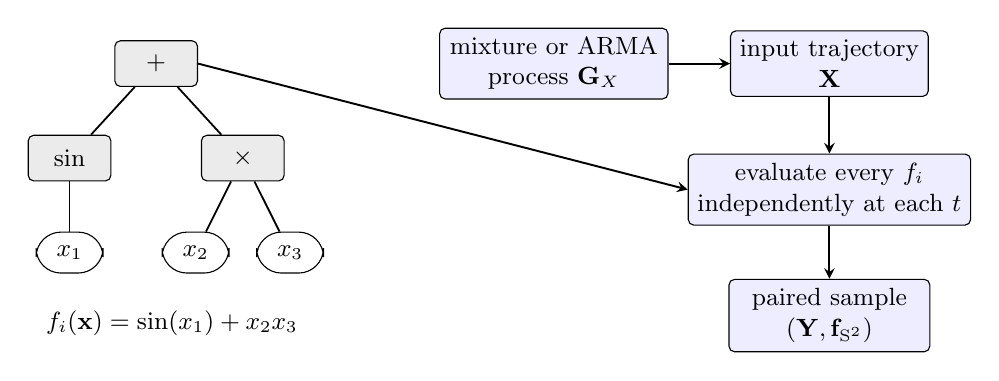
\begin{tikzpicture}[
    operator/.style={draw,rounded corners=2pt,fill=black!8,
        minimum width=1.05cm,minimum height=0.58cm,align=center,font=\small},
    leaf/.style={draw,rounded corners=9pt,fill=white,
        minimum width=0.85cm,minimum height=0.52cm,align=center,font=\small},
    block/.style={draw,rounded corners=2pt,fill=blue!7,
        minimum width=2.55cm,minimum height=0.72cm,align=center,font=\small},
    flow/.style={->,>=stealth,draw,line width=0.7pt},
    branch/.style={draw,line width=0.65pt}
]
    \node[operator] (add) at (-5.4,2.35) {$+$};
    \node[operator] (sin) at (-6.5,1.15) {$\sin$};
    \node[operator] (mul) at (-4.3,1.15) {$\times$};
    \node[leaf] (x1) at (-6.5,-0.05) {$x_1$};
    \node[leaf] (x2) at (-4.9,-0.05) {$x_2$};
    \node[leaf] (x3) at (-3.7,-0.05) {$x_3$};
    \draw[branch] (add)--(sin); \draw[branch] (add)--(mul);
    \draw[branch] (sin)--(x1);
    \draw[branch] (mul)--(x2); \draw[branch] (mul)--(x3);
    \node[font=\small,align=center] at (-5.2,-0.95)
        {$f_i(\mathbf x)=\sin(x_1)+x_2x_3$};

    \node[block,minimum width=2.9cm] (input) at (-0.35,2.35)
        {mixture or ARMA\\process $\mathbf G_X$};
    \node[block,minimum width=2.35cm] (X) at (3.15,2.35)
        {input trajectory\\$\mathbf X$};
    \node[block,minimum width=3.2cm] (f) at (3.15,0.75)
        {evaluate every $f_i$\\independently at each $t$};
    \node[block] (pair) at (3.15,-0.85)
        {paired sample\\$(\mathbf Y,\mathbf f_{\mathrm{S^2}})$};
    \draw[flow] (input)--(X);
    \draw[flow] (X)--(f);
    \draw[flow] (add.east) -- (f.west);
    \draw[flow] (f)--(pair);
\end{tikzpicture}
\caption{S$^2$Generator separates the sampled symbolic transformation from
the process that supplies its temporal inputs. The displayed tree acts on one
aligned input vector $\mathbf x_t$ at a time; mixture or ARMA sampling creates
the trajectory across $t$.}
\label{fig:s2-tree-and-series}
\end{figure}

\paragraph{How temporal inputs and outputs are produced.}
Every input channel is drawn either from a random finite mixture of Gaussian
or uniform distributions, or from a random-parameter ARMA$(p,q)$ process. In
the latter branch, the common notation gives

\begin{equation}
x_{j,t}=\sum_{r=1}^{p}a_{j,r}x_{j,t-r}
          +\eta_{j,t}
          -\sum_{s=1}^{q}\vartheta_{j,s}\eta_{j,t-s}.
\label{eq:s2-arma-input}
\end{equation}

The orders and coefficients are sampled within the bounds reported by the
paper, with constraints intended to favor stationary AR dynamics. Mixture
inputs provide varied marginal distributions; ARMA inputs additionally carry
serial dependence. Each channel of $\mathbf X$ is standardized, all trees are
evaluated pointwise according to Equation~\eqref{eq:s2-complete-generator},
and samples outside an operator's valid domain or with
$|y_{i,t}|>10^4$ are rejected. The released corpus contains 40 million
series--symbol pairs with a cumulative sequence length of 50 billion. For
fixed tree size, channel counts, mixture size, and ARMA orders, the authors'
analysis and timing experiment show generation cost approximately linear in
$T_{\mathrm{S^2}}$. Oversized random trees narrow valid domains and lower the
acceptance rate, which motivates the paper's bounded operator library.

\paragraph{How SymTime uses the pair.}
The time-series branch is a six-layer Transformer trained to reconstruct
masked non-overlapping patches. The symbolic branch is a six-layer DistilBERT
trained with masked-language modeling. Bidirectional series--symbol contrastive
loss aligns the two \texttt{[CLS]} representations, while momentum encoders
provide soft distillation targets. The total objective combines masked time
modeling, masked language modeling, contrastive alignment, and momentum
distillation. Fine-tuning uses the temporal encoder for long- and short-term
forecasting, classification, imputation, and anomaly detection. Thus, the
paired equation teaches a semantic representation; SymTime's decoder target
in downstream forecasting remains a future series rather than a recovered
prefix expression.

\paragraph{What is reused and what is new.}
Table~\ref{tab:s2-vs-symbolic-regression} shows that the tree data structure
and its random construction follow the established symbolic-regression
family. S$^2$Generator's contribution is the large-scale pairing of a sampled
algebraic map with a temporally structured multivariate stimulus, exhaustive
input/output dimensional coverage, and cross-modal pretraining on the
resulting series--symbol pairs.

\begin{table}[H]
\centering
\footnotesize
\renewcommand{\arraystretch}{1.06}
\begin{tabular}{@{}p{0.17\textwidth}p{0.27\textwidth}p{0.25\textwidth}p{0.23\textwidth}@{}}
\toprule
Work & Meaning of the sampled tree & Source of temporal dependence & Learned output \tabularnewline
\midrule
D'Ascoli et al. & Recurrence $u_n=F_{\mathcal T}(n,u_{n-1},\ldots)$ & Lagged sequence values are leaves of the tree & Recovered recurrence \tabularnewline
Me\v{z}nar et al. & General algebraic expression represented in a learned latent tree space & Defined by the later application of the expression & Expression optimized in latent space \tabularnewline
Bendinelli et al. & Static map $y=e(\mathbf x)$ paired with numerical support and hypotheses & A time-series adaptation would encode lags as input features & Recovered expression constrained by hypotheses \tabularnewline
ODEFormer & Vector field $\dot{\mathbf x}=\mathbf f(\mathbf x)$ & Numerical integration of the sampled field & Recovered differential equation \tabularnewline
S$^2$Generator and SymTime & Pointwise multivariate map $\mathbf y_t=\mathbf f_{\mathrm{S^2}}(\mathbf x_t)$ & Mixture or ARMA process $\mathbf G_X$ generates the input trajectory & Time-series representation aligned with symbolic semantics \tabularnewline
\bottomrule
\end{tabular}
\caption{The same broad unary--binary tree machinery receives different
temporal semantics and supports different learning objectives.}
\label{tab:s2-vs-symbolic-regression}
\end{table}

\paragraph{Explanation ground truth available to this thesis.}
The retained expression directly defines a contemporaneous structural mask

\begin{equation}
M^{\mathrm{S^2}}_{i,j}
=\mathbb I[x_j\text{ occurs in }f_i]
\label{eq:s2-structural-mask}
\end{equation}

and, wherever the sampled expression is differentiable, an exact local signed
sensitivity

\begin{equation}
J^{\mathrm{S^2}}_{i,j,t}
=\left.
\frac{\partial f_i(\mathbf x)}{\partial x_j}
\right|_{\mathbf x=\mathbf x_t}.
\label{eq:s2-local-jacobian}
\end{equation}

These references explain how the aligned stimulus $\mathbf x_t$ produces
$\mathbf y_t$. A variable--lag forecasting reference additionally requires
the ARMA mechanism in $\mathbf G_X$ and propagation of its lagged dependence
through $\mathbf f_{\mathrm{S^2}}$. Retaining both halves of
Equation~\eqref{eq:s2-complete-generator} would therefore strengthen the
proposed benchmark: the expression tree records the nonlinear cross-variable
transformation, while the sampled input-process record supplies temporal
memory. Extending the tree leaves themselves with
$\operatorname{LAG}(j,\ell)$ or recursive feedback would make temporal
dependencies explicit in one recorded mechanism.

The paper evaluates synthetic-data coverage using stationarity,
forecastability, mean FFT power, permutation entropy, seasonality, and trend.
It evaluates SymTime through downstream predictive tasks and representation
ablations. Direct equation-recovery accuracy and agreement
between XAI maps and generator-derived explanations lie outside that reported
protocol. For this thesis, S$^2$Generator is therefore chiefly a scalable
generator architecture and paired-data precedent; Equations
\eqref{eq:s2-structural-mask}--\eqref{eq:s2-local-jacobian} show the additional
references that can be derived once all sampled mechanisms are retained.

The official implementations are available in the S$^2$Generator repository
(\url{https://github.com/wwhenxuan/S2Generator}) and the SymTime repository
(\url{https://github.com/wwhenxuan/SymTime}).

\begin{table}[H]
\centering
\footnotesize
\renewcommand{\arraystretch}{1.04}
\begin{tabular}{@{}p{0.17\textwidth}p{0.31\textwidth}p{0.43\textwidth}@{}}
\toprule
Method & Retained synthetic mechanism & Scaling strategy and use in this thesis \\
\midrule
KernelSynth & Composite GP kernel $\kappa_\star$ & CPU-parallel GP draws and Arrow/LZ4 storage; supplies a covariance mechanism and exact conditional-mean gradient. \\
Chronos-2 & Base generator plus contemporaneous or sequential multivariatization & Patching, time/group attention, and a direct quantile head; motivates multivariate, lead--lag, and covariate-informed tasks. \\
TempoPFN and Toto 2.0 & Generator identity, sampled parameters, regimes, and augmentation chain & Mixed CPU/GPU priors plus Toto's CPM, u-$\mu$P, and FSDP2; motivates difficulty by regime, change point, long memory, and noise. \\
TimePFN/LMC-Synth & Latent GP kernels and Dirichlet mixing matrix & CPU-parallel sampling and channel-mixing attention; supplies known cross-channel covariance and a dense Jacobian reference. \\
S$^2$Generator and SymTime & Pointwise expression trees plus mixture/ARMA input processes & Approximately linear cost in sequence length for fixed mechanism size and paired series--symbol pretraining; supplies contemporaneous structure and a local Jacobian, while the retained input process adds temporal ground truth. \\
\bottomrule
\end{tabular}
\caption{Relationship between the synthetic pretraining methods, their
high-throughput implementations, and the proposed explanation benchmark.}
\label{tab:foundation-synthetic-comparison}
\end{table}



\subsection{Stability and Explosion Control in Recursive Generators}
\label{sec:explosion-treatment}

Recursive synthetic generators repeatedly feed their outputs back into the
next evaluation. Feedback can amplify perturbations and produce an explosive
trajectory. This subsection first grounds the implemented Jacobian-based
certificate through contraction, lag-state augmentation, robust invariance,
and random function iterations. It then reviews two additional foundations:
moment contraction for nonlinear autoregressions and a stationary
parameterization of multivariate linear autoregressions. Together they ground
four implemented comparison methods: the original random AST baseline, the
bounded-domain contraction generator, and generators adapted from each of
the two additional papers. Published mathematical results and the
benchmark adaptations are identified separately below.

Four properties guide the interpretation. An invariant domain keeps every
allowed trajectory inside a specified set. A uniform second-moment bound
controls expected squared magnitude over repeated realizations. Contraction
controls how differences between initial histories diminish under shared
future innovations. Strict stationarity means that joint probability laws
are unchanged by a time shift. A method can establish more than one of
these properties; each conclusion below is tied to its stated hypotheses.

\subsubsection{Contraction of Discrete-Time Nonlinear Systems}

\citet{tran2019convergence} compare convergence to one bounded trajectory
with incremental stability, which compares different trajectories.
Their Definition~6 controls small state perturbations through the Jacobian
in a uniformly bounded metric with a uniformly bounded inverse.
For the fixed nonsingular metric transformation $\Theta$ relevant to this
implementation, the transformed Jacobian is
\begin{equation}
 \mathcal J_\Theta(t,\mathbf{s})
 =\Theta J_{\mathcal F}(t,\mathbf{s})\Theta^{-1},
 \qquad
 \mathcal J_\Theta^\top\mathcal J_\Theta\preceq(1-\mu)I,
 \quad \mu>0.
\end{equation}
The transformation specifies how distances are measured. Theorem~15
relates contraction to exponential incremental stability; Theorem~16
adds compact positive invariance to obtain convergence to a unique bounded
trajectory. The benchmark uses a fixed induced norm and a convex invariant
box with $\sup_{\mathbf{s}\in D}\|J_{\mathcal F}(\mathbf{s})\|\leq\gamma<1$.
The derivative bound limits amplification of a difference along the entire
segment between two histories. With the same innovation at each future
step, repeated updates then decrease this difference geometrically.

\subsubsection{Lagged Recurrences as an Augmented State}

\citet{laraba2016setinvariance} review invariance for linear delay-difference
equations

\begin{equation}
    \mathbf x_{t+1}=\sum_{d=0}^{L-1}\mathbf C_{d+1}\mathbf x_{t-d}.
\end{equation}

$\mathbf C_{d+1}$ multiplies the vector at offset $d$; the next-target lag
is $\ell=d+1$. The authors
stack the current and delayed values into one state, so the delayed
equation becomes an ordinary first-order discrete-time system with a companion
transition matrix. They also define a delay-invariant set: if every initial lag
value lies in a set, every value subsequently produced by the recurrence stays
in that set. This supplies the appropriate state representation for an AST
whose leaves access several lags. In the nonlinear generator, the same idea is
used with $\mathbf{s}_t=(x_t,\ldots,x_{t-L+1})^\top$ and the set condition is
written directly as $\mathcal F_{\varepsilon}(D)\subseteq D$. The construction
extends to multivariate recurrences by stacking all $N$ variables at all $L$
lags into a state in $\mathbb R^{NL}$.

\subsubsection{Contraction with Stochastic Innovations}

\citet{kawano2024contraction} study systems
$\mathbf{s}_{t+1}=\mathcal F(\mathbf{s}_t,\xi_t)$.
Their incremental moment stability compares two trajectories under the same
stochastic realization and bounds the expected distance by a geometric
decay. Their Jacobian and metric conditions cover general stochastic
processes, with specializations for temporally independent and Markov
parameters.

The benchmark's bounded-domain method imposes a stronger, pathwise
condition: its Jacobian bound holds for every allowed state and every
innovation satisfying $|\varepsilon_t|\leq b_\varepsilon$.
With the same realized innovations, two histories therefore become
geometrically closer. A stationary long-run law additionally depends on
the update rule and the innovation process. The benchmark supplies a fixed
rule and i.i.d. innovations; the random-function result below provides
the corresponding distributional interpretation.

\subsubsection{Stationary Laws of Random Function Iterations}

\citet[Theorem~1]{diaconis1999iterated} represent a Markov chain as
$\mathbf{s}_{t+1}=\mathcal F_{\xi_{t+1}}(\mathbf{s}_t)$ with i.i.d.
random Lipschitz maps. On a complete separable metric space, the theorem
requires a finite expected Lipschitz factor, a finite expected displacement
from some reference state, and contraction on average:
\begin{equation}
 \mathbb E[\log K_\xi]<0.
\end{equation}
Here $K_\xi$ bounds the amplification of a state difference by the sampled
map. The conclusion is a unique stationary distribution and geometric
convergence in the Prokhorov distance, a distance between probability laws.
The benchmark's uniform bound $K_\xi\leq\gamma<1$, together with the
bounded invariant domain, supplies a stronger sufficient construction.
The result explains why persistent innovations can sustain fluctuations
while the distribution forgets the initial state. Forward simulations
approach a stationary law; coupling two starting histories with the same
noise gives a separate comparison of their realized paths.

\subsubsection{Shao and Wu: Moment Contraction for Nonlinear Time Series}
\label{sec:shao-wu-gmc}

\paragraph{Published result.}
\citet{shao2007spectral} develop spectral theory for nonlinear time series.
Section~5, Theorem~5.1 (pp.~11--12 of the linked electronic reprint), provides
the relevant generation result. With i.i.d. innovations and a measurable,
time-homogeneous recurrence $\mathcal R_{\mathcal T}(\mathbf{s};\varepsilon)$,
its second-moment specialization assumes a finite second moment at some
reference history and the global bound
\begin{equation}
\begin{split}
 \|\mathcal R_{\mathcal T}(\mathbf{s};\varepsilon)
       -\mathcal R_{\mathcal T}(\mathbf{s}';\varepsilon)\|_{L^2}
 &\leq \sum_{d=0}^{L-1}a_d^{\mathrm{GMC}}|s_d-s'_d|,\\
 a_d^{\mathrm{GMC}}\geq0,\qquad
 \sum_{d=0}^{L-1}a_d^{\mathrm{GMC}}&<1.
\end{split}
\label{eq:gmc-generator}
\end{equation}
Here $\|Z\|_{L^2}=(\mathbb E[\|Z\|_2^2])^{1/2}$. The theorem yields a
causal strictly stationary solution and geometric moment contraction (GMC):
the expected squared difference between coupled versions with a shared future
innovation sequence decays geometrically. Vector-valued states are admitted;
the absolute differences become norms of lag blocks. Theorem~5.2 preserves
GMC under stable ARMA filtering, and Examples~5.1--5.5 cover exponential
autoregression, conditional heteroscedasticity, and bilinear recursions.

\paragraph{Benchmark adaptation.}
The standard factor mode wraps lag leaves involved in nonlinear products
with $\tanh$, retains standalone linear terms, and scales the AST until
its global sensitivity budget is below one. For example, the drift
$0.3\tanh(x_t)\tanh(x_{t-1})$ has
derivative bounds $0.3$ for each lag, giving a total bound of $0.6$; Gaussian
innovations satisfy the required moment condition. This route targets
stationary nonlinear dynamics on an unbounded state space. Global derivative
bounds can overestimate sensitivity when repeated factors represent the
same historical coordinate. The alternative standard mode applies $\tanh$
after a complete product and checks the uniform amplitude moment bound
derived in Section~\ref{sec:implemented-shao-wu}. That bound is a project
construction with its own stated conclusion. The paper's GMC conclusion
applies when its global sensitivity and moment hypotheses are verified.
A finite
direct uniform initialization can leave a finite-horizon transient; its law
is recorded, and no preliminary path is simulated or discarded. The AST
sampling and certification rules are project adaptations; deriving compatible
explanation labels from the retained equations is a further benchmark step.

\subsubsection{Heaps: Stationary VAR Models through Reparameterization}
\label{sec:heaps-var}

\paragraph{Published result.}
\citet{heaps2023stationarity} constructs priors supported on stationary Gaussian
VAR models. For $\mathbf{x}_t=\sum_{\ell=1}^{L}\mathbf C_\ell
\mathbf{x}_{t-\ell}+\boldsymbol\varepsilon_t$, causal stationarity requires
the roots of \mbox{$\det(I-\sum_{\ell=1}^{L}\mathbf C_\ell z^\ell)=0$} to lie
outside the unit circle, equivalently $\rho(\mathbf B)<1$ for the companion
matrix $\mathbf B$. Sections~2.1--2.2 (pp.~3--5 of the arXiv version) map
unconstrained matrices to partial-autocorrelation matrices:
\begin{equation}
 \mathbf P_\ell^{\mathrm{PAC}}
 =\left(I+\mathbf U_\ell\mathbf U_\ell^\top\right)^{-1/2}\mathbf U_\ell,
 \qquad \ell=1,\ldots,L.
\label{eq:heaps-pac-map}
\end{equation}
The symmetric inverse square root maps a singular value $u\geq0$ to
$u/\sqrt{1+u^2}<1$. The Appendix (pp.~11--12) reconstructs the VAR coefficients
from these matrices and a positive-definite innovation covariance.
\citet{ansley1986reparameterizing} established the earlier unconstrained
parameterization; Heaps introduces symmetric square roots, a compatible
reverse recursion, and interpretable priors preserving useful symmetries.

\paragraph{Benchmark adaptation.}
The generator takes a specified innovation covariance
$\Sigma_{\varepsilon}\succ0$ and samples $\mathbf U_\ell$. It applies the
reverse recursion and stores the resulting $\mathbf C_\ell$ as linear ASTs.
Sampling the joint lag history from its stationary Gaussian law gives strict
and second-order stationarity from the first generated sample. Signed
coefficients and variable--lag support are read from the final equations.
Sections~3.3--3.4 distinguish shrinkage of intermediate parameters from
structural sparsity: isolated zeros generally change under the transformations.
Accordingly, support must be measured after reconstruction, and an imposed
coefficient mask requires renewed certification. The sampling distribution
also controls persistence and mechanism diversity. This method extends the
benchmark's earlier linear examples to jointly parameterized VAR models
with several variables and lags.

\subsubsection{Implications and Four Generator Strategies}
\label{sec:four-generator-strategies}

The AST families evaluate a retained deterministic expression as

\begin{equation}
    x_{t+1}
    =F_{\mathcal T}(x_t,\ldots,x_{t-L+1})+\varepsilon_{t+1}
\end{equation}

The bounded-domain constructor certifies the induced transition of the
augmented state. For
$D=[-r_D,r_D]^L$, interval propagation supplies both an output bound for
$F_{\mathcal T}$ and derivative bounds
$\overline d_d\ge
\sup_{\mathbf{s}\in D}|\partial F_{\mathcal T}/\partial s_d|$. With
$w_d=q_w^d$ and $q_w>1$, the corresponding weighted-infinity-norm bound is

\begin{equation}
    \gamma
    =\max\!\left\{
      \sum_{d=0}^{L-1}\overline d_d q_w^d,
      q_w^{-1}
    \right\}<1.
\end{equation}

The first term controls the nonlinear recurrence row of the Jacobian; the
second controls the deterministic shift of values through the lag state.
For $L=1$, there is no shift row and only the first term is used.
Bounded innovations are handled separately through the robust-invariance
condition

\begin{equation}
    \sup_{\mathbf{s}\in D}|F_{\mathcal T}(\mathbf{s})|
    +b_{\varepsilon}
    \le r_D,
\end{equation}

which ensures $\mathcal F_{\varepsilon}(D)\subseteq D$ for every admissible
innovation. Contraction therefore certifies exponential forgetting of the
initial history, invariance prevents escape from the certified domain, and the
random-iteration result supports a unique long-run distribution. Monte Carlo
simulation complements both certificates by diagnosing implementation errors
and measuring their conservatism.

These conditions are sufficient and intentionally conservative. A bounded
oscillatory mechanism may fail the uniform Jacobian test, interval arithmetic
may overestimate gains, and a hard invariant domain requires bounded noise.
The certificate consequently defines a controlled subset of the original AST
vocabulary whose trajectories can be generated with an explicit mathematical
stability guarantee.

Table~\ref{tab:four-generator-strategies} summarizes the implemented
comparison. The Shao--Wu factor mode and the bounded-domain method use
contraction with different domains and innovation assumptions. The
product-output mode checks its separately derived uniform second-moment
bound. Heaps provides a linear multivariate
parameterization over the causal stationary region. All four families are
evaluated in Section~\ref{sec:implemented-generator-results}.

\begingroup
\small
\renewcommand{\arraystretch}{1.12}
\begin{longtable}{@{}
>{\raggedright\arraybackslash}p{0.20\textwidth}
>{\raggedright\arraybackslash}p{0.34\textwidth}
>{\raggedright\arraybackslash}p{0.39\textwidth}@{}}
\caption{Four implemented generator strategies. Guarantees apply
under the stated domain, innovation, and initialization assumptions.}
\label{tab:four-generator-strategies}\\
\toprule
Method and status & Mechanism construction & Guarantee and principal trade-off\\
\midrule
\endfirsthead
\toprule
Method and status & Mechanism construction & Guarantee and principal trade-off\\
\midrule
\endhead
\bottomrule
\endlastfoot
Original random AST\newline Implemented &
Sample tree topology, operators, parameters, and lag bindings; execute the
recurrence. &
Empirical baseline with broad sampled algebraic structures; stability and
stationarity are assessed for each mechanism.\\
\addlinespace
Jacobian contraction\newline Implemented &
Scale the AST using interval bounds; certify a weighted lag-state Jacobian
and invariance of a bounded domain. &
Common-noise exponential forgetting and bounded trajectories in the certified
box. Current implementation: scalar series, bounded uniform innovations,
and sums/products.\\
\addlinespace
Shao--Wu family\newline Two standard modes &
Saturate factors and check the global sensitivity budget, or saturate the
complete product and check a growth envelope. &
Factor mode: causal stationary solution and GMC under Theorem~5.1.
Product-output mode: the derived uniform second-moment amplitude bound.
Both use directly sampled histories and Gaussian innovations.\\
\addlinespace
Heaps stationary VAR\newline Implemented &
Sample unconstrained matrices; transform to partial autocorrelations and
reconstruct VAR coefficients. &
Stationary Gaussian VAR($L$) with exact stationary initialization. Linear
interactions; final sparsity and persistence depend on the transformation.\\
\end{longtable}
\endgroup

The comparison reports explosion and near-zero rates together with
mechanism-sampling, certification, initialization, and trajectory-generation
times. Shared seeds, dimensions, lengths, and innovation variance support
matched experiments; innovation laws and supported mechanism families are
also reported. Numerical threshold crossings and finite-sample stationarity
diagnostics are empirical outcomes, while the certificates establish the
declared mathematical properties. Gaussian stationary trajectories can still
produce large excursions.

The benchmark will extract compatible explanation references from each
executable mechanism: variable--lag support, signed linear coefficients,
state-dependent term contributions, and derivatives. Multi-horizon
sensitivities propagate through the full recursion. SHAP references additionally
require a declared coalition and resampling rule.



\section{Research Goal and Research Question}

\subsection*{Motivation}

The project is intended to make the same synthetic generator useful both as a
\emph{prior} and as a \emph{benchmark}. Following the terminology used by
DoTime \citep{thumm2026dotime}, the prior is the distribution of synthetic
tasks used to train a model, while the benchmark provides fixed, reproducible
tasks for evaluation. Because the generating equations and sampled components
are known, the framework can provide supervision and evaluation references
that are difficult to obtain from real-world observations.

The framework will also allow researchers to construct synthetic scenarios
around the questions they want to investigate. They will be able to supply
equations within the supported vocabulary, provide initial conditions, or
configure the relationships and constraints used for random generation.
Alternatively, they may select an automatic generation method, such as a
VAR(1) generator or a nonlinear generator adapted from the framework of
\citet{shao2007spectral}. These methods represent examples of generation
strategies that the framework can accommodate as its capabilities evolve.

For each generated system, researchers will select the input series and
forecasting targets and control which information is provided to the model.
The roles of input and target will be defined separately from the dependencies
between series: inputs may depend on targets, and targets may depend on inputs
and on one another. Selected series may be hidden while remaining active in
the underlying generator. Future target values will be reserved as training
labels and evaluation references, while future values of selected input series
may be provided or withheld.

This flexibility will support controlled investigations of forecasting and
explainability methods. For example, a researcher could generate three
independent input series, allow only two to influence a target, and examine
whether a model uses the irrelevant input and whether an explanation method
reveals that behavior. Other experiments could hide a relevant series, change
the forecasting targets, or compare predictions with and without access to
future input values. Retaining the complete mechanism makes it possible to
distinguish the dependencies responsible for generating the data from those
used by the model.

As a benchmark, the generator will produce reproducible datasets with known
mechanisms and explanation references. Researchers will be able to compare
methods on the same trajectories under different information conditions and
examine how their performance changes across dependencies, lags, operators,
and forecast horizons. Depending on the outputs supported by each method,
evaluation will address forecasting accuracy, mechanism recovery, uncertainty
estimation, and explanation quality.

As a prior, the same framework could generate training examples with randomly
selected information conditions, allowing models to learn both to exploit
available future inputs and to forecast when those inputs are withheld. The
known mechanisms could also support pretraining beyond future-value
prediction. From a shared representation of the observed series, a model could
forecast the horizon, recover a symbolic equation, and estimate the
uncertainty associated with the innovations added at each step. The learnable
uncertainty concerns the expected distribution of future errors, whose
individual realizations remain random.

\begin{samepage}
Explanation ground truths will also support the training of explanation-aware
models. SHAPformer illustrates a related training strategy:
randomly masked feature coalitions allow the model to learn predictions from
different subsets of the input, supporting SHAP- and Owen-style explanations
at inference \citep{hertel2026shapformer}. Its synthetic ground-truth
explanations are used for evaluation. The proposed framework will support both
training with controlled information masks and direct supervision using
compatible explanation targets, enabling other architectures to learn
predictions, symbolic mechanisms, and explanations from the same synthetic
examples. Figure~\ref{fig:dual-prior-benchmark-motivation} illustrates one
multi-task architecture that these training examples could support.

\begin{figure}[H]
\centering
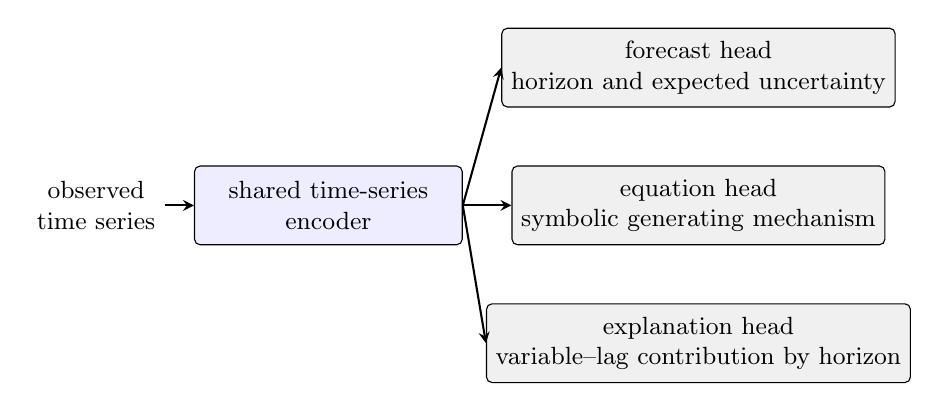
\begin{tikzpicture}[
    block/.style={draw,rounded corners=2pt,fill=blue!7,
        minimum width=3.4cm,minimum height=1.0cm,align=center,font=\small},
    head/.style={draw,rounded corners=2pt,fill=black!6,
        minimum width=4.1cm,minimum height=1.0cm,align=center,font=\small},
    flow/.style={->,>=stealth,draw,line width=0.75pt}
]
    \node[font=\small,align=center] (input) at (-5.2,0)
        {observed\\time series};
    \node[block] (encoder) at (-2.25,0)
        {shared time-series\\encoder};
    \node[head] (forecast) at (2.45,1.75)
        {forecast head\\horizon and expected uncertainty};
    \node[head] (equation) at (2.45,0)
        {equation head\\symbolic generating mechanism};
    \node[head] (explanation) at (2.45,-1.75)
        {explanation head\\variable--lag contribution by horizon};

    \draw[flow] (input)--(encoder);
    \draw[flow] (encoder.east)--(forecast.west);
    \draw[flow] (encoder.east)--(equation.west);
    \draw[flow] (encoder.east)--(explanation.west);
\end{tikzpicture}
\caption{Conceptual multi-task model enabled by the synthetic prior. A shared
time-series encoder feeds a forecasting head for future values and expected
uncertainty, an equation-recovery head, and an explanation head. The generator
supplies the corresponding supervision, while the benchmark retains the
mechanisms and explanation references for evaluation.}
\label{fig:dual-prior-benchmark-motivation}
\end{figure}
\end{samepage}

% Evidence: ChatTS, Sections 3.2--3.5, pp. 2388--2390, and Section 4.6,
% p. 2393; LLaVA, Sections 4.1--4.2, PDF pp. 4--5, Figure 1 and Eq. (1).
The generated data could also support future applications in which large
language models (LLMs) analyze time series through explanations and learned
temporal representations. ChatTS
illustrates the importance of this representation: it aligns a time-series
encoder with an LLM using synthetic series, attribute descriptions, and
question--answer pairs, and reports limitations when the same temporal data
are supplied only as text \citep[Sections~3.2--3.5 and 4.6]{xie2025chatts}.
The resulting series--explanation pairs could be reused in two complementary
ways. First,
explanations of variable--lag dependencies and contributions could be provided
as text or structured context to guide an LLM's analysis of a series. Second,
explanation ground truths could supervise a time-series encoder during
training, encouraging it to retain information about these dependencies.
A learned projection could then connect its representations to the LLM's
input embedding space through \emph{multimodal alignment}. LLaVA provides an
image-based example: a visual encoder produces features that a trained
projection maps into a sequence of embeddings consumed by the language model
\citep[Sections~4.1--4.2]{liu2023visual}. Such reuse could ultimately improve
temporal representations and LLM-based analysis, extending the value of the
generated supervision to future multimodal applications.

\subsection{Research Goal}

The goal of this thesis is to design, implement, and validate a configurable
synthetic benchmark for discrete-time time series. Each dataset will be
produced by a fully known generative mechanism from which several compatible
levels of explanation ground truth can be derived. The benchmark will support
the systematic evaluation of three method families: forecasting models,
symbolic system-identification methods, and XAI techniques. The central
evaluation question is whether these methods recover, use, and explain the
true temporal dependencies of the process.

The generator family will progress from simple to more demanding mechanisms,
including autoregressive dependencies, cross-variable and variable--lag
interactions, nonlinear terms, multiple temporal scales, regime changes,
irrelevant variables, and stochastic components. Depending on the mechanism,
the resulting references will include binary structural dependencies, exact
signed coefficients, realized local coefficient--input contributions, and
attribution-based explanations such as generator-level Shapley values. These
references will be indexed at the target, source-variable, lag, instance, and,
when the generator produces multiple future values, forecast-horizon levels.

Following the expression-first strategy of \citet{dascoli2022deep} and the
learned tree-prior alternative of \citet{meznar2023efficient}, the formula
sampler will construct a valid symbolic tree before generating observations.
The retained tree will act as an executable data-generating function and as the
mechanism record from which the benchmark derives its structural,
coefficient-level, local-contribution, and attribution-based references.
Following \citet{bendinelli2023controllable}, an optional retrieval protocol
will expose controlled subsets of this record as hypotheses and measure how
mechanism recovery changes when prior information is complete, partial,
missing, or partially incorrect.

The resulting framework will provide controlled and reproducible comparisons
of predictive accuracy, mechanism recovery, and explanation accuracy. It will
also support tests of whether a black-box forecaster relies on the same
temporal relationships as the true generator or as a symbolic model identified
independently from the generated observations.

\subsection{\texorpdfstring{\hspace{0.45em}Research Question}{Research Question}}

\begin{quote}
\textbf{How can synthetic discrete-time time-series generators with known
generative mechanisms and explanation ground truths be used to benchmark the
ability of forecasting, system-identification, and explainability methods to
recover, use, and explain the underlying temporal dependencies?}
\end{quote}

\paragraph{Three sources of disagreement.}
Let $x$ be a forecasting input, $g$ the known generator, $f$ a forecaster
trained on observations from $g$, and $\widehat g$ a symbolic mechanism
identified independently from those observations. The benchmark separates the
following quantities:

\begin{align}
\varepsilon_{\mathrm{forecast}}(x)
&=d_y\!\left(f(x),g(x)\right),
\label{eq:forecast-error}\\
\varepsilon_{\mathrm{mechanism}}^{*}
&=d_{\mathcal M}\!\left(\mathcal M(\widehat g),\mathcal M(g)\right),
\label{eq:mechanism-error}\\
\varepsilon_{\mathrm{explanation}}(x)
&=d_{\mathcal E}\!\left(A(f,x),E_f(x)\right).
\label{eq:explanation-error}
\end{align}

\noindent\textsuperscript{*}\emph{Applicability of the mechanism error:}
this quantity is evaluated when the method exposes an explicit representation
$\mathcal M(\cdot)$ that can be aligned with the known generator, as occurs in
symbolic system-identification methods and explainable-by-design forecasters.
For an explainable-by-design forecaster, $\mathcal M(\widehat g)$ in
Eq.~\ref{eq:mechanism-error} is replaced by $\mathcal M(f)$. Post-hoc
attribution methods are evaluated through the explanation comparisons in
Eqs.~\ref{eq:explanation-error}--\ref{eq:symbolic-agreement}.

Equation~\ref{eq:forecast-error} measures whether the forecaster returns the
same future values as the generator. Equation~\ref{eq:mechanism-error} measures
whether system identification recovers the generator's structure, lags,
coefficients, nonlinear terms, and regimes at the level represented by
$\mathcal M$. Equation~\ref{eq:explanation-error} measures whether an XAI
method faithfully describes the mechanism actually used by the trained
forecaster; $E_f(x)$ denotes the corresponding model-level reference.

An explainable-by-design forecaster that exposes generator-compatible
source--lag coefficients can also be evaluated through
$d_{\mathcal M}(\mathcal M(f),\mathcal M(g))$, as in the coefficient-recovery
setting studied with DCIts \citep{baric2026dcits}. For a black-box forecaster,
two additional comparisons answer complementary questions:

\begin{align}
\varepsilon_{\mathrm{generator\ agreement}}(x)
&=d_{\mathcal E}\!\left(A(f,x),E_g(x)\right),
\label{eq:generator-agreement}\\
\varepsilon_{\mathrm{symbolic\ agreement}}(x)
&=d_{\mathcal E}\!\left(A(f,x),E_{\widehat g}(x)\right).
\label{eq:symbolic-agreement}
\end{align}

The first comparison tests end-to-end agreement between the black-box
explanation and the true process explanation; it combines any mismatch learned
by $f$ with the behavior of the XAI method. The second tests agreement with an
independently recovered symbolic explanation; its interpretation is paired
with the mechanism-identification error in Eq.~\ref{eq:mechanism-error}. A
small symbolic-agreement error becomes evidence about the true mechanism when
$\widehat g$ also achieves a small mechanism-identification error. Together,
these quantities separate accurate forecasting, recovery of the generating
rule, and faithful explanation of the predictor while allowing their
relationships to be studied explicitly.

\subsection{Benchmark Requirements}
\label{sec:benchmark-requirements}

The benchmark requirements distinguish three kinds of commitment. A
\emph{core requirement} defines behavior that the first complete library must
provide; a \emph{research requirement} identifies a methodological decision
that must be resolved and documented during development; and an
\emph{extension point} keeps the implementation open to later additions
without expanding the experimental scope of this thesis. This distinction is
important because the principal contribution is the generation of executable
time-series mechanisms and their explanation ground truths. General-purpose
grammar design and unrestricted user-defined operators remain extension
points.

\subsubsection{Fixed grammar and reproducible mechanism sampling}

\paragraph{R1: fixed and versioned grammar.}
The project will define one fixed initial vocabulary of constants, lagged
variables, unary operators, binary operators, and mechanism-level constructs.
Users will configure how mechanisms are sampled from this vocabulary, while
the vocabulary itself remains controlled by the project. Every generated
dataset will record a grammar version. Internally, operators will be
registered through a modular interface so that later versions can extend the
grammar without changing the public contract of the first benchmark.

\paragraph{R2: deterministic random generation.}
A global seed, complete generation configuration, library version, and
execution backend will determine the generated mechanisms, coefficients,
initial conditions, innovations, trajectories, windows, and stochastic
explanation estimates. Each artifact will receive a named random stream
derived from stable identifiers such as the mechanism, trajectory, window,
and explanation method. Consequently, changing the number of data-loading
workers or their completion order will preserve the identity and contents of
every indexed example. Repeated execution on the same backend will target
bitwise equality; comparisons across numerical backends will use a declared
floating-point tolerance.

\paragraph{R3: separation between mechanisms and trajectories.}
A mechanism record will contain the expression tree, lag assignments,
coefficients, noise law, and any regime-transition rule. One mechanism may
generate several trajectories. These trajectories share the same symbolic
tree and sampled mechanism parameters while using independently seeded initial
conditions and innovation realizations. This hierarchy supports the study of
whether a method recovers a persistent generating rule rather than properties
of one particular realization:
\[
\boxed{
\text{mechanism}
\longrightarrow
\{\text{trajectory}_{1},\ldots,\text{trajectory}_{K}\}
\longrightarrow
\{\text{forecasting windows}\}.
}
\]
Each window will retain identifiers linking it to its trajectory and sampled
mechanism.

\subsubsection{Controlled and randomly covered difficulty}

\paragraph{R4: two complementary descriptions of difficulty.}
The benchmark will store both \emph{designed difficulty}, determined by the
sampled mechanism, and \emph{measured difficulty}, determined from the
realized forecasting task. Designed difficulty includes tree depth, operator
count, interaction order, number of active variables, lag distance, temporal
scales, recursion depth, regime changes, and the configured noise level.
Measured difficulty includes forecastability statistics, oracle uncertainty,
and the excess error of a fixed panel of reference forecasters over the known
generator.

This separation avoids treating all hard examples as equivalent. A
white-noise process has a simple structural rule but high irreducible
uncertainty, whereas a noiseless nonlinear recurrence can be structurally
complex while remaining deterministic. Difficulty is therefore recorded for
a specified input length, observed-variable set, loss, and horizon. The same
trajectory can be easy at $h=1$ and difficult at a longer horizon.

Related work supplies useful but complementary precedents. SynTSBench controls
temporal pattern families, irregularities, dependencies, and theoretical
optima in order to diagnose forecasting capabilities
\citep{tan2025syntsbench}. The difficulty-conditioned generator of
\citet{cazaux2026synthetic} uses a scalar to alter component balance,
harmonics, regime changes, and noise, and samples named easy, medium, hard, and
uniform distributions. Its downstream ablation also shows that generator
difficulty labels alone need not create proportionally separated forecasting
errors. Data-driven forecastability can additionally be characterized through
spectral predictability and Lyapunov stability \citep{wang2025forecastability}
or through the task-aligned spectral-coherence score of
\citet{feng2025predictability}. These results motivate calibration rather than
assigning difficulty from expression size alone.

\paragraph{R5: random generation with calibrated coverage.}
The default benchmark suite will first sample a target difficulty stratum and
then sample mechanisms from its internal prior. A calibration stage will
measure the realized examples, adjust or relabel them, and freeze versioned
thresholds. The released suite will report the intended stratum and the
measured difficulty descriptors, permitting both a balanced easy--medium--hard
comparison and analysis along the individual axes. Establishing the precise
calibration score and thresholds is a research requirement of the thesis.

\subsubsection{Horizon-aware explanation ground truths}

\paragraph{R6: a separate reference for every forecast step.}
Every explanation ground truth will retain the forecast-horizon axis. For a
source variable $j$, historical offset $d$, and forecast step $h$, the
reference answers whether and how $x_{j,\tau-d}$ affects $g_h(x)$. The chosen
tensor organization is therefore
\[
\boxed{
\text{example}\times
\text{target}\times
\text{horizon}\times
\text{source variable}\times
\text{historical offset},
}
\]
with additional value or method dimensions only when required by a specific
ground-truth family. Aggregation over $h$ will be a reported summary rather
than a replacement for the horizon-resolved reference.

\paragraph{R7: propagation through recursive rollouts.}
When a later forecast uses an earlier generated value, its explanation will be
propagated back to the original observed window. For example, if $g_2(x)$ uses
$g_1(x)$, its input gradient includes both a direct path and the path through
the first forecast:
\begin{equation}
\frac{\partial g_2(x)}{\partial x_{j,\tau-d}}
=
\left.
\frac{\partial g_2(x)}{\partial x_{j,\tau-d}}
\right|_{\mathrm{direct}}
+
\frac{\partial g_2(x)}{\partial g_1(x)}
\frac{\partial g_1(x)}{\partial x_{j,\tau-d}}.
\label{eq:recursive-gradient-requirement}
\end{equation}
Repeated application of Eq.~\eqref{eq:recursive-gradient-requirement}
propagates differentiable effects through the complete rollout. Structural
references will propagate Boolean reachability through the same computation
graph. Generator-level Shapley values will define the value function using the
complete $h$-step rollout, so that coalitions are evaluated directly for the
requested horizon. This is required because Shapley values from consecutive
nonlinear forecast steps cannot in general be combined by simple addition.

\paragraph{R8: selectable ground truths.}
Users will request the ground-truth families needed by an experiment. Binary
structural support can be derived from every retained expression graph. Signed
coefficients apply to mechanisms with identifiable coefficient parameters;
realized local contributions apply when the expression admits a declared
decomposition; and gradients apply to differentiable operators under a stated
policy for nondifferentiable points. Generator-level Shapley values apply to an
executable generator but may require exact enumeration, permutation sampling,
or specialized estimators depending on the number of players. The library will
record the estimator, baseline or conditional sampler, approximation budget,
and uncertainty of every stochastic reference. Gradient feasibility and the
treatment of discontinuities and regime switches are research requirements.

\subsubsection{Model-independent evaluation and explanation metrics}

\paragraph{R9: universal forecasting-model adapter.}
The evaluation layer will interact with a predictor through a small adapter
contract for fitting when required, prediction, and optional explanation or
mechanism retrieval. The contract will represent zero-shot foundation models,
trainable global or local models, statistical models, and
explainable-by-design forecasters. Each adapter will publish capabilities such
as multivariate input, known future covariates, probabilistic output,
automatic differentiation, native explanation, and explicit mechanism
retrieval. Dataset generation and metric implementations will remain
independent of model-specific code.

\paragraph{R10: metrics matched to explanation semantics.}
The benchmark will provide several \emph{explainability} metrics for each
compatible reference family. Binary source--lag masks will use support and
ranking measures such as precision, recall, F1, area under the precision--recall
curve, and top-$k$ recovery. Signed coefficients and signed local references
will additionally use normalized value error and sign agreement. Continuous
attributions will use magnitude error, rank correlation, top-$k$ overlap, sign
agreement, and completeness residuals when completeness belongs to the
attribution definition. Metrics will first be computed per example and
horizon; macro- and micro-aggregated results will be reported separately to
avoid allowing frequent or long mechanisms to dominate every summary.

\paragraph{R11: capability-aware separation of errors.}
Forecast error in Eq.~\eqref{eq:forecast-error} applies whenever an adapter
returns predictions. Explanation comparisons apply when an explainer or model
returns an output aligned with a supported reference. Mechanism-identification
error in Eq.~\eqref{eq:mechanism-error} applies when a method exposes an
explicit, alignable representation. The library will return applicability
metadata alongside every metric rather than filling unsupported comparisons
with inferred values. The exact user-facing adapter and result interfaces, and
the boundary between model-level fidelity and generator agreement, form a
research requirement to be resolved through executable prototypes.

\subsubsection{Lazy, parallel, and batched generation}

\paragraph{R12: PyTorch-compatible on-demand dataset.}
The primary dataset interface will follow the indexed
\texttt{torch.utils.data.Dataset} contract. An index will deterministically
identify a mechanism, trajectory, and forecasting window; requesting that
index will generate or retrieve its values and the selected explanation
ground truths. This map-style interface supports exact replay, stable
train--validation--test partitions, caching, and comparison of multiple models
on identical examples.

The dataset will integrate with \texttt{DataLoader} workers so that future
batches are generated concurrently while the current batch is consumed. The
implementation will support worker processes, custom collation, batch
prefetching, persistent workers, and pinned host memory as described in the
official PyTorch data-loading interface.\footnote{PyTorch data-loading
documentation: \url{https://docs.pytorch.org/docs/stable/data.html}.}
A typical use will have the following form:

\begin{lstlisting}[language=Python,caption={Required lazy and parallel batch-generation interface.}]
dataset = SyntheticExplanationDataset(
    seed=42,
    num_mechanisms=1000,
    trajectories_per_mechanism=10,
    context_length=512,
    prediction_length=96,
    ground_truths=["structural_mask", "gradient"],
)

loader = DataLoader(
    dataset,
    batch_size=64,
    num_workers=8,
    prefetch_factor=2,
    persistent_workers=True,
    pin_memory=True,
    collate_fn=dataset.collate,
)

for batch in loader:
    forecast = model(batch["past_values"])
    report.update(forecast, batch)
\end{lstlisting}

The collated batch will contain the past window, future target, requested
horizon-resolved ground truths, and identifiers for the formula, mechanism,
trajectory, and window. Expensive explanation references will be computed only
when requested and may be stored in a bounded cache. A later streaming
interface may use \texttt{IterableDataset} for effectively unlimited
pretraining data; the indexed dataset remains the reference implementation for
benchmark comparisons.

\paragraph{R13: performance characterization and scalable execution.}
Performance experiments will compare sequential CPU generation,
vectorized CPU execution, CPU multiprocessing, and batched GPU execution.
They will measure examples and batches per second, latency, peak host and
device memory, accelerator utilization, cache hit rate, and the cost of each
ground-truth family. CPU workers will normally produce host tensors and pinned
memory will support asynchronous device transfer. GPU-native generation will
use a controlled batched execution path rather than independent CUDA contexts
inside data-loader workers. The final configuration will preserve the stable
sample identity defined by R2 for every tested worker count and backend.

\subsubsection{Ground-truth correctness and acceptance criteria}

\paragraph{R14: correctness tests for generated references.}
The implementation will include tests of the benchmark's own reference
construction. Executing the stored mechanism must reproduce its deterministic
trajectory before innovations are added; expression leaves must agree with the
structural mask; analytical or automatic gradients must agree with finite
differences away from nondifferentiable points; and multi-horizon toy
recurrences must verify recursive path propagation. Where the attribution
definition requires efficiency, the baseline plus attributed contributions
must reconstruct the relevant output within the estimator's declared
tolerance. Seed, cache, batching, and parallel-worker tests must reproduce the
same indexed examples. These checks establish the internal correctness of the
ground truths before they are used to judge forecasting or explanation
methods.

Table~\ref{tab:benchmark-requirements} summarizes the resulting acceptance
contract.

\begingroup
\small
\renewcommand{\arraystretch}{1.08}
\begin{longtable}{@{}
>{\raggedright\arraybackslash}p{0.08\textwidth}
>{\raggedright\arraybackslash}p{0.42\textwidth}
>{\raggedright\arraybackslash}p{0.42\textwidth}@{}}
\caption{Requirements and acceptance evidence for the proposed benchmark.}
\label{tab:benchmark-requirements}\\
\toprule
ID & Required behavior & Acceptance evidence \\
\midrule
\endfirsthead
\multicolumn{3}{@{}l}{\small\emph{Table~\thetable\ continued}}\\
\toprule
ID & Required behavior & Acceptance evidence \\
\midrule
\endhead
\midrule
\multicolumn{3}{r@{}}{\small\emph{Continued on the next page}}\\
\endfoot
\bottomrule
\endlastfoot
R1 & Fixed, documented, and versioned initial grammar. & Every dataset records its grammar version and every sampled tree validates against that version. \\
R2 & Deterministic named random streams. & Equal configuration, seed, version, and backend produce equal sample hashes; worker count does not change indexed examples. \\
R3 & Multiple trajectories from one retained mechanism. & Trajectories share the tree and mechanism parameters while initial conditions and innovations vary reproducibly. \\
R4 & Separate designed complexity from realized forecastability. & Both descriptor groups are stored per mechanism, trajectory, task, and horizon where applicable. \\
R5 & Random generation covering easy, medium, and hard cases. & A versioned calibration protocol reports intended strata, measured descriptors, thresholds, and final counts. \\
R6 & Horizon-resolved explanation references. & Every supported reference exposes target, horizon, source, and historical-offset axes before aggregation. \\
R7 & Recursive explanation propagation. & Analytical multi-step recurrences verify gradients, structural paths, and complete-rollout attribution behavior. \\
R8 & Optional ground-truth families with explicit applicability. & Output metadata records the reference definition, estimator, configuration, uncertainty, and unsupported cases. \\
R9 & Model-independent evaluation adapter. & Statistical, zero-shot, trainable, black-box, and explainable-by-design examples use the same evaluation entry point. \\
R10 & Explanation-specific metric families. & Binary, signed, ranked, and local-valued references are evaluated only with semantically compatible metrics. \\
R11 & Capability-aware error decomposition. & Reports distinguish computed, unsupported, and inapplicable forecast, mechanism, and explanation comparisons. \\
R12 & Lazy parallel batch generation. & A PyTorch DataLoader generates and prefetches batches without materializing the complete dataset and without duplicated samples. \\
R13 & Measured CPU/GPU performance. & Reproducible profiles report throughput, latency, memory, utilization, caching, and ground-truth cost. \\
R14 & Internal ground-truth correctness tests. & Stored mechanisms, masks, gradients, recursive paths, attributions, seeds, and caches pass automated consistency checks. \\
\end{longtable}
\endgroup

\clearpage

\section{Research Plan}

\subsection{Scope of the November 2026 minimum viable benchmark}

The target for 30 November 2026 is a tested Python library rather than a
single experiment script. Its minimum viable release will (i) sample valid
discrete-time formulas, (ii) execute them to generate reproducible datasets,
(iii) derive several explanation ground truths from the retained formulas,
(iv) accept forecasting models through a small adapter interface, and
(v) produce comparable forecasting and explanation reports. The first release
will prioritize deterministic autoregressive, cross-variable, nonlinear, and
irrelevant-input mechanisms. Regime switching and stochastic mechanisms will
enter the release only after the deterministic path passes its validation
tests, because they introduce additional questions about state labels,
innovation terms, and the object to be explained.

The first stochastic generator will use additive zero-mean Gaussian
innovations with a sampled scale. This initial restriction makes the expected
error distribution explicit and testable. Additional innovation families,
including heavy-tailed, heteroscedastic, and regime-dependent noise, will be
considered after the Gaussian generator and its evaluation interface pass the
validation gates.

The intended dependency order is
\[
\boxed{
\begin{gathered}
\text{formula AST}
\longrightarrow
\text{executable generator}
\longrightarrow
\text{time-series dataset}
\\[1mm]
\Downarrow
\\[1mm]
\text{explanation ground truths}
\longrightarrow
\text{model adapters}
\longrightarrow
\text{evaluation}
\end{gathered}
}.
\]
Consequently, model experiments do not begin before both the observations and
their references can be generated and checked. A lightweight software
interface is specified early so that the generator does not become tied to one
forecasting package, but the interface is exercised on real models only after
the ground-truth layer is complete.

\subsection{Formula sampler}

Following the expression-first strategy of \citet{dascoli2022deep}, the
sampler will first create an abstract syntax tree (AST) and only then execute
it. Let $\mathcal E$ denote a valid symbolic expression, either the complete
right-hand side of a recurrence or one of its subexpressions. A minimal
recursive grammar is
\[
\begin{aligned}
\mathcal E ::= {}& c
&& \text{sampled constant,}\\
&\mid \operatorname{LAG}(j,\ell)
&& \text{series $j$ observed $\ell$ steps earlier,}\\
&\mid \operatorname{ADD}(\mathcal E_1,\mathcal E_2)
&& \text{sum of two valid expressions,}\\
&\mid \operatorname{MUL}(\mathcal E_1,\mathcal E_2)
&& \text{product of two valid expressions,}\\
&\mid \operatorname{UNARY}_{\varphi}(\mathcal E_1)
&& \text{unary function applied to one expression,}
\end{aligned}
\qquad \ell\geq 1.
\]
The symbol $\mathcal E$ is therefore a grammar non-terminal: it is a
placeholder for any expression that can be constructed by repeatedly applying
these rules. The symbols $\mathcal E_1$ and $\mathcal E_2$ are child
expressions constructed by the same grammar, $c$ is a sampled constant, $j$
identifies a source series, and $\varphi$ is selected from a controlled set of
unary functions. The initial vocabulary fixes $\varphi=\tanh$;
Section~\ref{sec:generator-vocabulary} specifies its terminals and operators.

For example, the symbolic tree
\[
\begin{aligned}
\mathcal E={}&\operatorname{ADD}\!\bigl(
    \operatorname{MUL}(0.7,\operatorname{LAG}(1,1)),\\
&\hspace{38mm}\operatorname{TANH}(\operatorname{LAG}(1,3))
\bigr)
\end{aligned}
\]
is executed as the recurrence
\[
x_{1,t}=0.7x_{1,t-1}+\tanh(x_{1,t-3}).
\]
Extensions will add explicit interaction, regime, multiscale, and innovation
nodes. The AST is retained alongside every series as the executable description
of the mechanism; a rendered equation is a human-readable view of that same
object.

The sampler must control tree depth, operator counts, admissible domains,
maximum lag, coefficient ranges, and duplicated or inactive branches. Candidate
formulas are rejected when short pilot simulations diverge, collapse to an
almost constant series, produce non-finite values, or fail to use the sampled
dependencies. Each accepted formula is serialized with its seed and complete
parameter record so that it can be reconstructed exactly.

\subsection{Series generation and dataset contract}

For target series $k$, the AST is compiled into an executable recurrence
\[
x_{k,t}=g_{k,1}\!\left(x_{:,t-1},\ldots,x_{:,t-L};\theta\right)
       +\varepsilon_{k,t}.
\]
Initial conditions are sampled first, trajectories are generated recursively,
and the observations are divided chronologically into training, validation,
and test windows. The generator records the formula, coefficients, initial
conditions, innovations, regime sequence when applicable, seeds, window
boundaries, and temporal convention. This metadata distinguishes the process
that generated the observations from the input window later presented to a
model.

Multi-step reference outputs are produced by recursively executing the known
generator. Thus $g_{k,h}$ denotes the output at horizon $h$ after unrolling the
one-step recurrence $h$ times. The benchmark will expose the same sample through
a benchmark batch containing observed history, optional known future
covariates, target values, horizon, masks, and metadata. An adapter may transform
that batch into a package-specific dataframe or tensor, but it cannot silently
change which information the model receives.

\subsection{Explanation ground truths}

Only after an accepted formula and its observations exist does the library
derive explanation references. One generated example can expose four
compatible views:

\begin{enumerate}
    \item a binary source--lag support extracted from the AST and, for
    $h>1$, from the recursively unrolled dependency graph;
    \item signed coefficients for mechanisms whose effect is represented by a
    coefficient, together with realized coefficient--input terms;
    \item a local gradient reference
    \[
    G^{\mathrm{grad}}_{n,h,j,d}
      =\frac{\partial g_{k,h}(x_n)}
             {\partial x_{j,\tau-d}},
    \]
    computed by automatic differentiation when the sampled operators are
    differentiable and checked against finite differences; and
    \item generator-level Shapley values obtained by evaluating the executable
    generator under feature coalitions and a declared conditional resampling
    rule; when the benchmark declares a hierarchy of player groups, the same
    game also yields Owen values that respect that grouping.
\end{enumerate}

The raw gradient measures local sensitivity. A baseline-relative
gradient--input quantity,
$(x_{j,\tau-d}-b_{j,d})G^{\mathrm{grad}}_{n,h,j,d}$, may also be stored, but it
will be named separately because it is a contribution heuristic rather than a
Shapley value. Comparisons remain within the same explanation family: a model
gradient is compared with the generator gradient, while a model SHAP
explanation is compared with the generator SHAP reference. Exact Shapley
enumeration will validate small cases; permutation sampling and caching will be
used when the number of players makes enumeration impractical.

\subsection{Model-independent evaluation layer}

The public boundary of the benchmark is a \texttt{ForecastAdapter}. Every
adapter declares its input capabilities and implements fitting, prediction,
and, when available, access to an intrinsic mechanism or differentiable model.
The evaluator will therefore distinguish three cases:

\begin{itemize}
    \item every adapter can be evaluated for forecast accuracy;
    \item any callable predictor can receive model-agnostic perturbation or
    finite-difference explanations;
    \item mechanism-recovery metrics are computed only when a method exposes a
    generator-compatible structure, equation, coefficient tensor, or other
    explicit mechanism. Unsupported cells are reported as not applicable, not
    as zero performance.
\end{itemize}

The initial integration set comprises Chronos-2
\citep{ansari2025chronos2}, Toto 2.0 from Datadog
\citep{khwaja2026toto2}, AutoARIMA \citep{hyndman2008auto}, and, as an
optional explainable-by-design baseline, DCIts \citep{baric2026dcits}. The
planning name ``Kronos-2'' is normalized here to \emph{Chronos-2}; Kronos is a
different foundation model specialized for financial-market sequences.
Chronos-2 and Toto 2.0 are evaluated as pretrained forecasters through their
adapters. AutoARIMA is evaluated first with target-only history; a separate
ARIMAX configuration can later receive declared exogenous variables. DCIts
provides a learned transition tensor rather than a symbolic equation, so its
native coefficients can be compared with compatible generator references.

Forecast metrics will include MAE, RMSE, and MASE. Structural recovery will use
precision, recall, and F1 over source--lag support. Coefficient recovery will
use signed error and sign agreement when such coefficients exist. Local
explanation comparisons will include normalized attribution error, rank
correlation, top-$q$ overlap, and sign agreement. All results will retain the
instance, target, horizon, source variable, lag, operator family, formula
complexity, and random seed required for stratified analysis.

\subsection{Validation gates}

The release is accepted only if (i) AST parsing and serialization round-trip
without changing a formula, (ii) seeded generation is reproducible, (iii)
hand-derived support, coefficient, contribution, gradient, and small Shapley
examples match the implementation, (iv) one-step and recursively unrolled
horizon references are separated, (v) all model adapters receive the declared
input only, and (vi) the complete pipeline runs from configuration file to
tables without notebook-only state. These gates protect the benchmark from
producing precise-looking metrics for an incorrectly represented mechanism.

\subsection{Weekly plan}

Table~\ref{tab:weekly-plan} places formula and series generation before the
explanation layer, and places the model study after both. Each week ends in a
testable artifact rather than an open-ended research activity.

Figure~\ref{fig:research-plan-gantt} presents the same plan as a dependency-aware
Gantt chart. Solid arrows mark hard gates. The dashed region identifies work
that can proceed in parallel once the executable generator has passed its first
validation gate; the adapter contract begins earlier from the frozen data
contract, but its implementation converges with the dataset and explanation
branches before model integration.

\begin{landscape}
\begin{figure}[H]
    \centering
    \resizebox{0.98\linewidth}{!}{%
        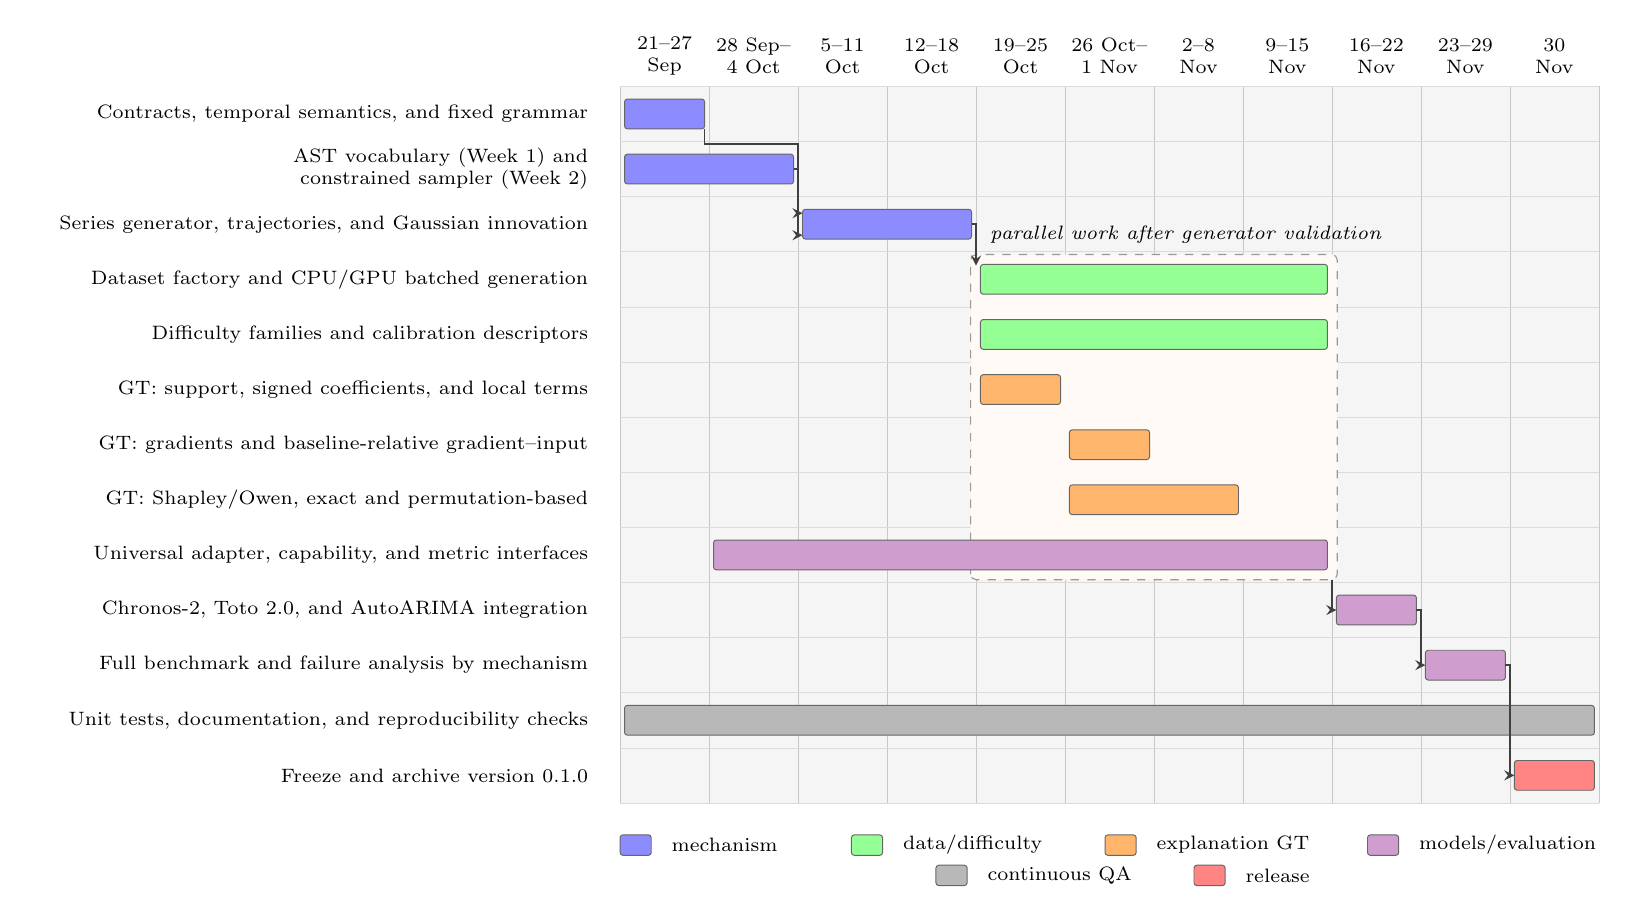
\begin{tikzpicture}[
    x=1.13cm,
    y=0.70cm,
    tasklabel/.style={font=\scriptsize,anchor=east,align=right,text width=7.0cm},
    bar/.style={draw=black!60,line width=0.35pt,rounded corners=1pt},
    dependency/.style={->,>=stealth,semithick,draw=black!75},
    legend/.style={font=\scriptsize,anchor=west}
]

% Timeline grid.
\fill[black!4] (0,-0.5) rectangle (11,12.5);
\foreach \x in {0,...,11} {
    \draw[black!22,line width=0.25pt] (\x,-0.5) -- (\x,12.5);
}
\foreach \y in {-0.5,0.5,...,12.5} {
    \draw[black!14,line width=0.2pt] (0,\y) -- (11,\y);
}

% Week headings.
\node[font=\scriptsize,align=center] at (0.5,13.05) {21--27\\Sep};
\node[font=\scriptsize,align=center] at (1.5,13.05) {28 Sep--\\4 Oct};
\node[font=\scriptsize,align=center] at (2.5,13.05) {5--11\\Oct};
\node[font=\scriptsize,align=center] at (3.5,13.05) {12--18\\Oct};
\node[font=\scriptsize,align=center] at (4.5,13.05) {19--25\\Oct};
\node[font=\scriptsize,align=center] at (5.5,13.05) {26 Oct--\\1 Nov};
\node[font=\scriptsize,align=center] at (6.5,13.05) {2--8\\Nov};
\node[font=\scriptsize,align=center] at (7.5,13.05) {9--15\\Nov};
\node[font=\scriptsize,align=center] at (8.5,13.05) {16--22\\Nov};
\node[font=\scriptsize,align=center] at (9.5,13.05) {23--29\\Nov};
\node[font=\scriptsize,align=center] at (10.5,13.05) {30\\Nov};

% Task labels.
\node[tasklabel] at (-0.25,12) {Contracts, temporal semantics, and fixed grammar};
\node[tasklabel] at (-0.25,11) {AST vocabulary (Week 1) and constrained sampler (Week 2)};
\node[tasklabel] at (-0.25,10) {Series generator, trajectories, and Gaussian innovation};
\node[tasklabel] at (-0.25,9) {Dataset factory and CPU/GPU batched generation};
\node[tasklabel] at (-0.25,8) {Difficulty families and calibration descriptors};
\node[tasklabel] at (-0.25,7) {GT: support, signed coefficients, and local terms};
\node[tasklabel] at (-0.25,6) {GT: gradients and baseline-relative gradient--input};
\node[tasklabel] at (-0.25,5) {GT: Shapley/Owen, exact and permutation-based};
\node[tasklabel] at (-0.25,4) {Universal adapter, capability, and metric interfaces};
\node[tasklabel] at (-0.25,3) {Chronos-2, Toto 2.0, and AutoARIMA integration};
\node[tasklabel] at (-0.25,2) {Full benchmark and failure analysis by mechanism};
\node[tasklabel] at (-0.25,1) {Unit tests, documentation, and reproducibility checks};
\node[tasklabel] at (-0.25,0) {Freeze and archive version 0.1.0};

% Parallel work window after the first validated generator.
\filldraw[fill=orange!4,draw=black!40,dashed,rounded corners=2pt]
    (3.94,3.55) rectangle (8.06,9.45);
\node[font=\scriptsize\itshape,anchor=south west] at (4.05,9.48)
    {parallel work after generator validation};

% Core mechanism construction.
\filldraw[bar,fill=blue!45] (0.05,11.73) rectangle (0.95,12.27);
\filldraw[bar,fill=blue!45] (0.05,10.73) rectangle (1.95,11.27);
\filldraw[bar,fill=blue!45] (2.05,9.73) rectangle (3.95,10.27);

% Scalable generation and controlled difficulty.
\filldraw[bar,fill=green!42] (4.05,8.73) rectangle (7.95,9.27);
\filldraw[bar,fill=green!42] (4.05,7.73) rectangle (7.95,8.27);

% Explanation-ground-truth methods.
\filldraw[bar,fill=orange!58] (4.05,6.73) rectangle (4.95,7.27);
\filldraw[bar,fill=orange!58] (5.05,5.73) rectangle (5.95,6.27);
\filldraw[bar,fill=orange!58] (5.05,4.73) rectangle (6.95,5.27);

% Evaluation interface and model study.
\filldraw[bar,fill=violet!38] (1.05,3.73) rectangle (7.95,4.27);
\filldraw[bar,fill=violet!38] (8.05,2.73) rectangle (8.95,3.27);
\filldraw[bar,fill=violet!38] (9.05,1.73) rectangle (9.95,2.27);

% Continuous quality work and final milestone.
\filldraw[bar,fill=black!28] (0.05,0.73) rectangle (10.95,1.27);
\filldraw[bar,fill=red!48] (10.05,-0.27) rectangle (10.95,0.27);

% Hard dependency gates.
\draw[dependency] (0.95,11.73) -- (0.95,11.45) -- (2.00,11.45)
    -- (2.00,10.20) -- (2.05,10.20);
\draw[dependency] (1.95,11) -- (2.00,11) -- (2.00,9.80) -- (2.05,9.80);
\draw[dependency] (3.95,10) -- (4.00,10) -- (4.00,9.25);
\draw[dependency] (8.00,3.55) -- (8.00,3) -- (8.05,3);
\draw[dependency] (8.95,3) -- (9.00,3) |- (9.05,2);
\draw[dependency] (9.95,2) -- (10.00,2) -- (10.00,0) -- (10.05,0);

% Legend, split over two rows to remain readable after page scaling.
\filldraw[bar,fill=blue!45] (0,-1.45) rectangle (0.35,-1.08);
\node[legend] at (0.47,-1.265) {mechanism};
\filldraw[bar,fill=green!42] (2.60,-1.45) rectangle (2.95,-1.08);
\node[legend] at (3.07,-1.265) {data/difficulty};
\filldraw[bar,fill=orange!58] (5.45,-1.45) rectangle (5.80,-1.08);
\node[legend] at (5.92,-1.265) {explanation GT};
\filldraw[bar,fill=violet!38] (8.40,-1.45) rectangle (8.75,-1.08);
\node[legend] at (8.87,-1.265) {models/evaluation};

\filldraw[bar,fill=black!28] (3.55,-2.00) rectangle (3.90,-1.63);
\node[legend] at (4.02,-1.815) {continuous QA};
\filldraw[bar,fill=red!48] (6.45,-2.00) rectangle (6.80,-1.63);
\node[legend] at (6.92,-1.815) {release};

\end{tikzpicture}
%
    }
    \caption{Dependency-aware Gantt plan for the benchmark release on
    30 November 2026. The explanation-ground-truth branch explicitly covers
    binary source--lag support, signed coefficients and realized local terms,
    automatic-differentiation gradients and gradient--input values, and
    generator-level Shapley values or Owen values for grouped players. Exact
    coalition enumeration is used for small games and permutation estimation
    for larger games.}
    \label{fig:research-plan-gantt}
\end{figure}
\end{landscape}

\begin{landscape}
\begin{figure}[H]
    \centering
    \resizebox{0.77\linewidth}{!}{%
        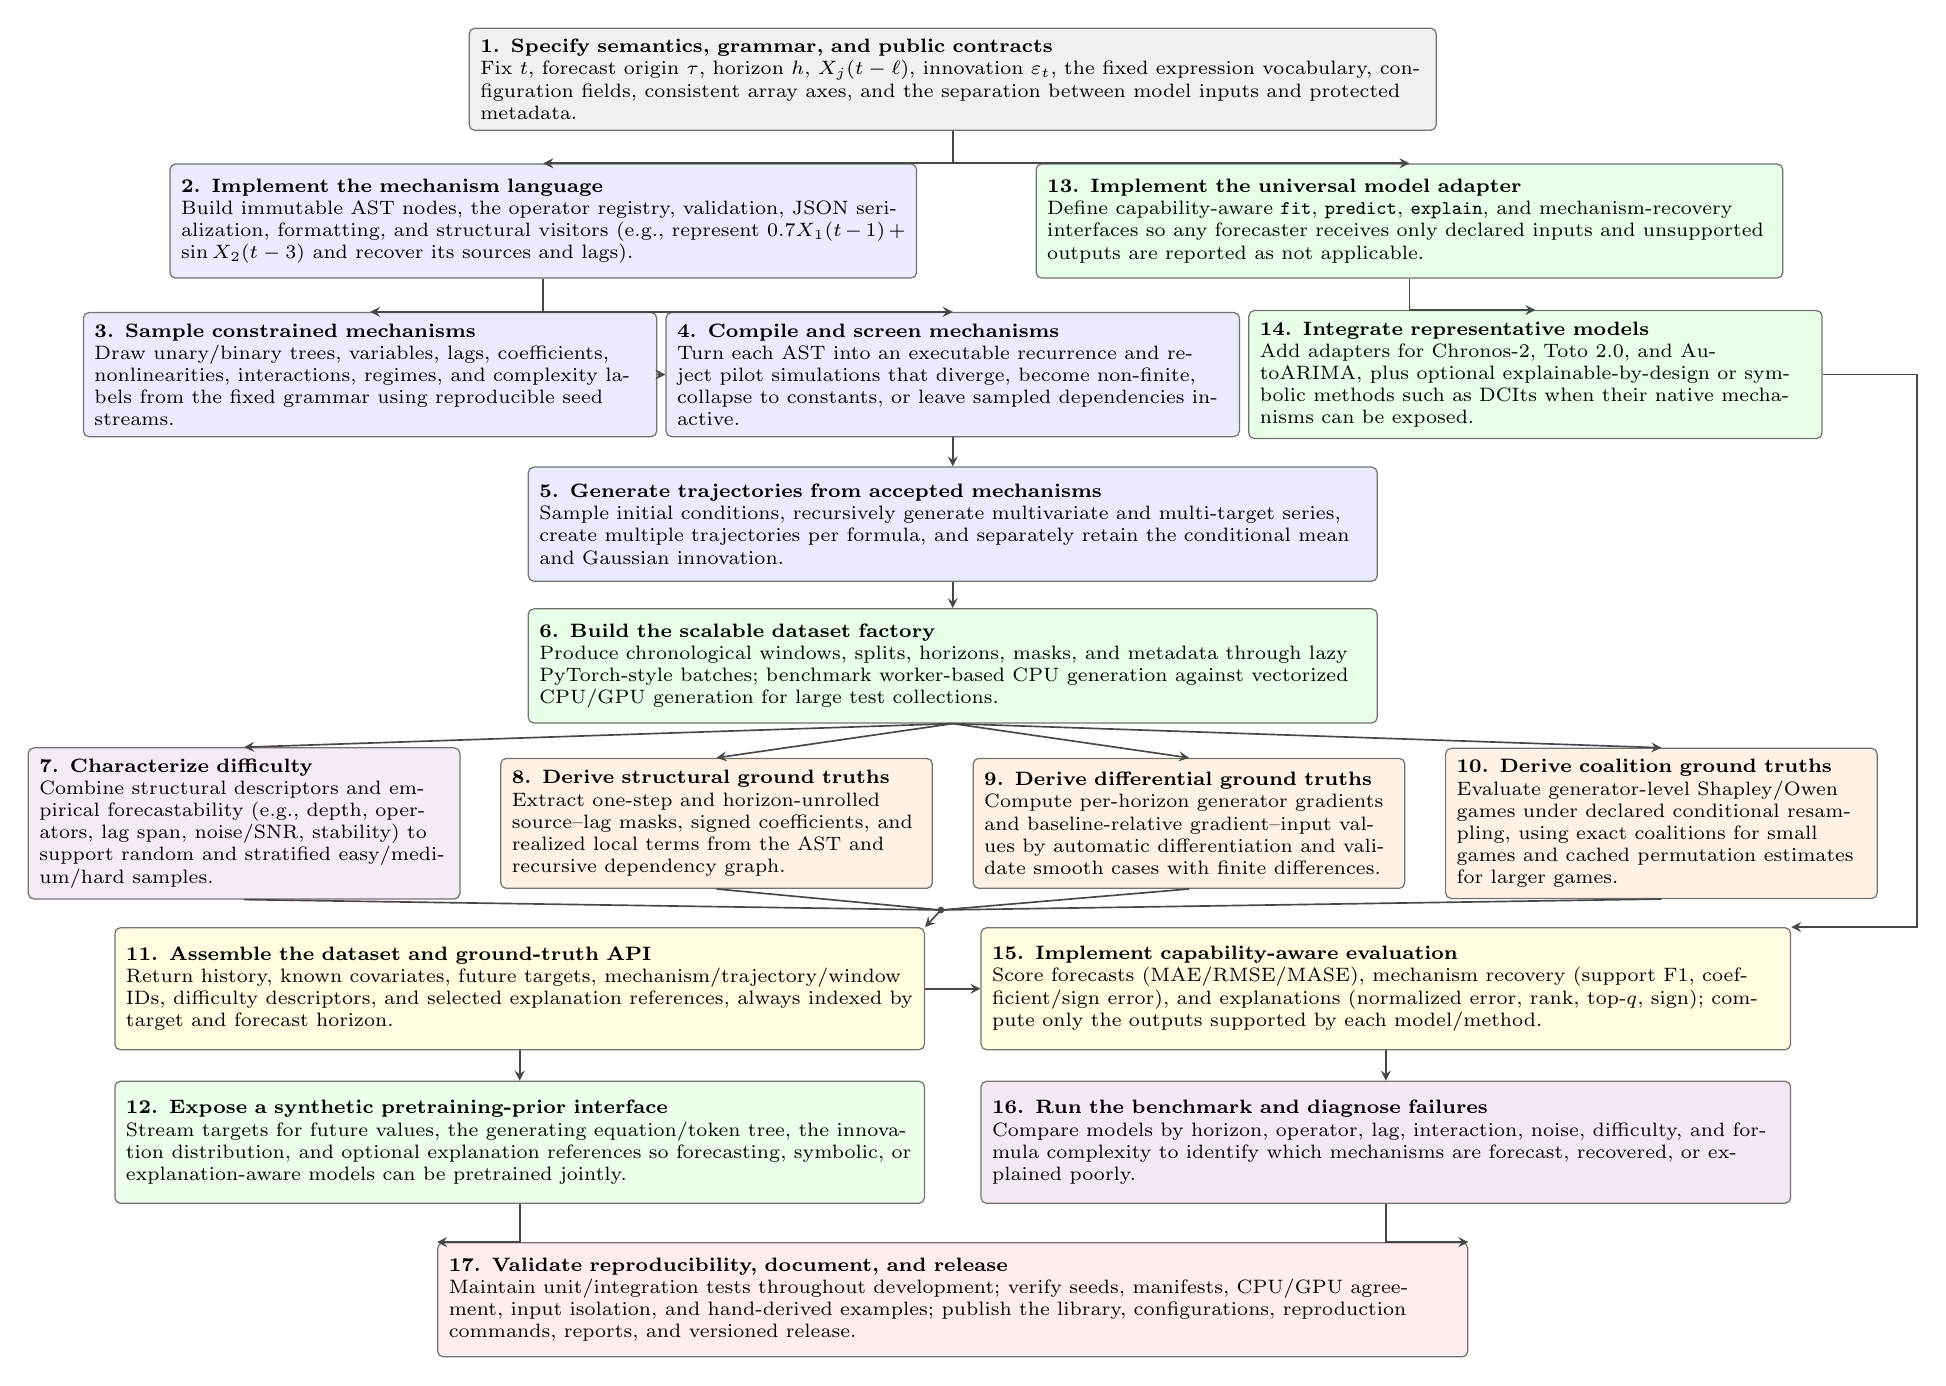
\begin{tikzpicture}[
    x=1cm,
    y=1cm,
    task/.style={
        draw=black!55,
        line width=0.45pt,
        rounded corners=2pt,
        align=left,
        inner sep=4pt,
        font=\scriptsize
    },
    dependency/.style={->,>=stealth,semithick,draw=black!72},
    joinline/.style={semithick,draw=black!72}
]

% Shared scientific and software foundation.
\node[task,fill=black!6,text width=12.0cm,minimum height=1.25cm] (specification) at (0,7.4) {%
    \textbf{1. Specify semantics, grammar, and public contracts}\par
    Fix $t$, forecast origin $\tau$, horizon $h$, $X_j(t-\ell)$, innovation
    $\varepsilon_t$, the fixed expression vocabulary, configuration fields,
    consistent array axes, and the separation between model inputs and protected metadata.
};

\node[task,fill=blue!8,text width=9.2cm,minimum height=1.45cm] (language) at (-5.2,5.6) {%
    \textbf{2. Implement the mechanism language}\par
    Build immutable AST nodes, the operator registry, validation, JSON serialization,
    formatting, and structural visitors (e.g., represent
    $0.7X_1(t-1)+\sin X_2(t-3)$ and recover its sources and lags).
};

% The adapter boundary can start from the public contracts while generators are built.
\node[task,fill=green!9,text width=9.2cm,minimum height=1.45cm] (adapter) at (5.8,5.6) {%
    \textbf{13. Implement the universal model adapter}\par
    Define capability-aware \texttt{fit}, \texttt{predict}, \texttt{explain}, and
    mechanism-recovery interfaces so any forecaster receives only declared inputs and
    unsupported outputs are reported as not applicable.
};

\node[task,fill=blue!8,text width=7.0cm,minimum height=1.55cm] (sampler) at (-7.4,3.65) {%
    \textbf{3. Sample constrained mechanisms}\par
    Draw unary/binary trees, variables, lags, coefficients, nonlinearities,
    interactions, regimes, and complexity labels from the fixed grammar using
    reproducible seed streams.
};

\node[task,fill=blue!8,text width=7.0cm,minimum height=1.55cm] (compiler) at (0,3.65) {%
    \textbf{4. Compile and screen mechanisms}\par
    Turn each AST into an executable recurrence and reject pilot simulations that
    diverge, become non-finite, collapse to constants, or leave sampled dependencies
    inactive.
};

\node[task,fill=green!9,text width=7.0cm,minimum height=1.55cm] (models) at (7.4,3.65) {%
    \textbf{14. Integrate representative models}\par
    Add adapters for Chronos-2, Toto~2.0, and AutoARIMA, plus optional
    explainable-by-design or symbolic methods such as DCIts when their native
    mechanisms can be exposed.
};

\node[task,fill=blue!8,text width=10.5cm,minimum height=1.45cm] (trajectories) at (0,1.75) {%
    \textbf{5. Generate trajectories from accepted mechanisms}\par
    Sample initial conditions, recursively generate multivariate and
    multi-target series, create multiple trajectories per formula, and separately
    retain the conditional mean and Gaussian innovation.
};

\node[task,fill=green!9,text width=10.5cm,minimum height=1.45cm] (dataset) at (0,-0.05) {%
    \textbf{6. Build the scalable dataset factory}\par
    Produce chronological windows, splits, horizons, masks, and metadata through lazy
    PyTorch-style batches; benchmark worker-based CPU generation against vectorized
    CPU/GPU generation for large test collections.
};

% Parallel products derived from the retained mechanism and generated observations.
\node[task,fill=violet!8,text width=5.2cm,minimum height=1.65cm] (difficulty) at (-9.0,-2.05) {%
    \textbf{7. Characterize difficulty}\par
    Combine structural descriptors and empirical forecastability (e.g., depth,
    operators, lag span, noise/SNR, stability) to support random and stratified
    easy/medium/hard samples.
};

\node[task,fill=orange!10,text width=5.2cm,minimum height=1.65cm] (structural) at (-3.0,-2.05) {%
    \textbf{8. Derive structural ground truths}\par
    Extract one-step and horizon-unrolled source--lag masks, signed coefficients, and
    realized local terms from the AST and recursive dependency graph.
};

\node[task,fill=orange!10,text width=5.2cm,minimum height=1.65cm] (gradient) at (3.0,-2.05) {%
    \textbf{9. Derive differential ground truths}\par
    Compute per-horizon generator gradients and baseline-relative gradient--input
    values by automatic differentiation and validate smooth cases with finite
    differences.
};

\node[task,fill=orange!10,text width=5.2cm,minimum height=1.65cm] (coalition) at (9.0,-2.05) {%
    \textbf{10. Derive coalition ground truths}\par
    Evaluate generator-level Shapley/Owen games under declared conditional resampling,
    using exact coalitions for small games and cached permutation estimates for larger
    games.
};

\node[task,fill=yellow!12,text width=10.0cm,minimum height=1.55cm] (datasetapi) at (-5.5,-4.15) {%
    \textbf{11. Assemble the dataset and ground-truth API}\par
    Return history, known covariates, future targets, mechanism/trajectory/window IDs,
    difficulty descriptors, and selected explanation references, always indexed by
    target and forecast horizon.
};

\node[task,fill=yellow!12,text width=10.0cm,minimum height=1.55cm] (evaluation) at (5.5,-4.15) {%
    \textbf{15. Implement capability-aware evaluation}\par
    Score forecasts (MAE/RMSE/MASE), mechanism recovery (support F1, coefficient/sign
    error), and explanations (normalized error, rank, top-$q$, sign); compute only the
    outputs supported by each model/method.
};

% Two intended uses of the generated data and ground truths.
\node[task,fill=green!8,text width=10.0cm,minimum height=1.55cm] (prior) at (-5.5,-6.10) {%
    \textbf{12. Expose a synthetic pretraining-prior interface}\par
    Stream targets for future values, the generating equation/token tree, the
    innovation distribution, and optional explanation references so forecasting,
    symbolic, or explanation-aware models can be pretrained jointly.
};

\node[task,fill=violet!9,text width=10.0cm,minimum height=1.55cm] (benchmark) at (5.5,-6.10) {%
    \textbf{16. Run the benchmark and diagnose failures}\par
    Compare models by horizon, operator, lag, interaction, noise, difficulty, and
    formula complexity to identify which mechanisms are forecast, recovered, or
    explained poorly.
};

\node[task,fill=red!7,text width=12.8cm,minimum height=1.45cm] (release) at (0,-8.10) {%
    \textbf{17. Validate reproducibility, document, and release}\par
    Maintain unit/integration tests throughout development; verify seeds, manifests,
    CPU/GPU agreement, input isolation, and hand-derived examples; publish the library,
    configurations, reproduction commands, reports, and versioned release.
};

% Hard technical dependencies.
\draw[dependency] (specification.south) -- ++(0,-0.22) |- (language.north);
\draw[dependency] (specification.south) -- ++(0,-0.22) |- (adapter.north);

\draw[dependency] (language.south) -- ++(0,-0.22) |- (sampler.north);
\draw[dependency] (language.south) -- ++(0,-0.22) |- (compiler.north);
\draw[dependency] (sampler.east) -- (compiler.west);
\draw[dependency] (compiler.south) -- (trajectories.north);
\draw[dependency] (trajectories.south) -- (dataset.north);

\draw[dependency] (adapter.south) -- ++(0,-0.22) |- (models.north);

\draw[dependency] (dataset.south) -- (difficulty.north);
\draw[dependency] (dataset.south) -- (structural.north);
\draw[dependency] (dataset.south) -- (gradient.north);
\draw[dependency] (dataset.south) -- (coalition.north);

\coordinate (productjoin) at (-0.15,-3.15);
\draw[joinline] (difficulty.south) -- (productjoin);
\draw[joinline] (structural.south) -- (productjoin);
\draw[joinline] (gradient.south) -- (productjoin);
\draw[joinline] (coalition.south) -- (productjoin);
\fill[black!72] (productjoin) circle (1.2pt);
\draw[dependency] (productjoin) -- (datasetapi.north east);

\draw[dependency] (datasetapi.south) -- (prior.north);
\draw[dependency] (datasetapi.east) -- (evaluation.west);
\draw[dependency] (models.east) -- ++(1.2,0) |- (evaluation.north east);
\draw[dependency] (evaluation.south) -- (benchmark.north);

\draw[dependency] (prior.south) -- ++(0,-0.22) |- (release.north west);
\draw[dependency] (benchmark.south) -- ++(0,-0.22) |- (release.north east);

\end{tikzpicture}
%
    }
    \caption{Overall technical dependency graph for the project.  The retained
    symbolic mechanism drives trajectory generation, difficulty characterization,
    and structural, differential, and coalition-based explanation references.  The
    resulting API supports two consumers: synthetic pretraining priors and a
    model-agnostic benchmark with capability-aware forecast, mechanism-recovery,
    and explanation evaluation.}
    \label{fig:project-dependency-graph}
\end{figure}
\end{landscape}

\begingroup
\small
\setlength{\LTpre}{0.4\baselineskip}
\setlength{\LTpost}{0.7\baselineskip}
\renewcommand{\arraystretch}{1.08}
\begin{longtable}{@{}
>{\raggedright\arraybackslash}p{0.14\textwidth}
>{\raggedright\arraybackslash}p{0.25\textwidth}
>{\raggedright\arraybackslash}p{0.28\textwidth}
>{\raggedright\arraybackslash}p{0.25\textwidth}@{}}
\caption{Dependency-aware schedule for a usable benchmark by 30 November 2026.}
\label{tab:weekly-plan}\\
\toprule
Dates & Main work & Deliverable & Acceptance criterion \\
\midrule
\endfirsthead
\multicolumn{4}{@{}l}{\small\emph{Table~\thetable\ continued}}\\
\toprule
Dates & Main work & Deliverable & Acceptance criterion \\
\midrule
\endhead
\midrule
\multicolumn{4}{r@{}}{\small\emph{Continued on the next page}}\\
\endfoot
\bottomrule
\endlastfoot

21--27 Sep. &
Freeze temporal semantics, AST schema, operator registry, and configuration
contract. &
Grammar specification, Python types, and hand-written reference formulas. &
At least 30 representative formulas parse, serialize, and preserve their
source--lag identities. \\

28 Sep.--4 Oct. &
Implement constrained random AST sampling and formula rejection filters. &
Seeded formula sampler with complexity and operator labels. &
A batch of 10,000 candidates is reproducible; every accepted formula is
causal, finite in pilot execution, and reconstructible from metadata. \\

5--11 Oct. &
Compile ASTs and implement initial conditions, recursive simulation,
and multivariate output. &
Executable deterministic generator and unit tests. &
Repeated seeds reproduce identical series; simple AR, cross-lag, and nonlinear
examples match hand calculations. \\

12--18 Oct. &
Create dataset splits and controlled families for interactions, irrelevant
variables, lag ranges, and temporal scales. &
Versioned dataset factory and data cards. &
Every sample links back to one formula; leakage checks pass and all information
available to a model is recorded explicitly. \\

19--25 Oct. &
Extract structural support, signed coefficients where defined, realized local
terms, and horizon-unrolled dependencies. &
First ground-truth API and visual sanity reports. &
Hand-derived one-step and multi-step examples match the stored masks and
values exactly. \\

26 Oct.--1 Nov. &
Implement generator gradients and baseline-relative gradient--input outputs. &
Gradient reference module indexed by instance, horizon, variable, and lag. &
Autodiff agrees with central finite differences on smooth formulas; undefined
or non-smooth cases are flagged rather than silently scored. \\

2--8 Nov. &
Implement coalition construction, dependency-aware resampling, exact small
Shapley cases, and permutation estimates. &
Generator SHAP reference module with uncertainty and sampling metadata. &
Exact and sampled results agree within a declared tolerance on small formulas,
and efficiency is checked whenever the chosen game satisfies it. \\

9--15 Nov. &
Implement adapter protocols, forecast/mechanism/explanation metrics, capability
checks, and result schema. &
End-to-end library pipeline using naive and oracle test adapters. &
One configuration produces datasets, references, predictions, explanations,
and stratified tables without notebook state. \\

16--22 Nov. &
Integrate Chronos-2, Toto 2.0, and target-only AutoARIMA; add DCIts if the core
path remains on schedule. &
Model adapters and a common pilot experiment. &
Every model sees the documented context and horizon; unsupported mechanism
metrics are marked not applicable. \\

23--29 Nov. &
Run the comparison matrix; analyze error by operator, lag range, horizon,
interaction, and irrelevant-variable count; finish tests and documentation. &
Release candidate, examples, metric tables, and reproducibility manifest. &
A clean environment can reproduce the principal tables from one command and
all mandatory tests pass. \\

30 Nov. &
Freeze and archive version 0.1.0. &
Installable package, tagged configuration set, generated artifacts, and usage
example. &
The release checklist and a full smoke test pass from installation through
report export. \\
\end{longtable}
\endgroup

\subsection{Final goal: using the benchmark as a library}

The final user should configure a generator once and evaluate multiple models
without changing the data-generation or scoring code. Listing~\ref{lst:final-api}
illustrates the intended public API. The adapter classes belong to the proposed
library; internally, they translate the benchmark batch to the
official input expected by each external package.

\begin{lstlisting}[language=Python,caption={Intended end-state API for generating one benchmark and evaluating the prioritized models.},label={lst:final-api}]
from tsxai_benchmark import Benchmark, GeneratorSpec
from tsxai_benchmark.ground_truth import (
    StructuralSupport,
    SignedCoefficients,
    LocalContributions,
    GeneratorGradient,
    GradientInput,
    GeneratorShapley,
)
from tsxai_benchmark.models import (
    Chronos2Adapter,
    Toto2Adapter,
    AutoARIMAAdapter,
    DCItsAdapter,
)
from tsxai_benchmark.xai import InputGradient, PermutationSHAP

# 1. Sample formulas, execute them, and retain every mechanism.
benchmark = Benchmark.generate(
    GeneratorSpec(
        n_formulas=500,
        series_length=1024,
        context_length=256,
        horizon=24,
        max_lag=48,
        operators=["add", "multiply", "tanh"],
        include_irrelevant_variables=True,
        seed=42,
    ),
    ground_truths=[
        StructuralSupport(unroll_horizon=True),
        SignedCoefficients(when_defined=True),
        LocalContributions(),
        GeneratorGradient(),
        GradientInput(baseline="training_mean"),
        GeneratorShapley(
            masker="generator_conditional",
            permutations=512,
        ),
    ],
)

# 2. Model-specific details are isolated inside adapters.
models = [
    Chronos2Adapter(model_id="amazon/chronos-2"),
    Toto2Adapter(model_id="Datadog/Toto-2.0-22m"),
    AutoARIMAAdapter(
        season_length=24,
        input_mode="target_only",
    ),
    # Optional explainable-by-design baseline.
    DCItsAdapter(context_length=48),
]

# 3. Like is compared with like: gradients with gradients,
#    and SHAP values with generator-level Shapley values.
report = benchmark.evaluate(
    models=models,
    explainers={
        "gradient": InputGradient(fallback="finite_difference"),
        "shap": PermutationSHAP(
            masker=benchmark.conditional_sampler,
            permutations=512,
        ),
    },
    forecast_metrics=["mae", "rmse", "mase"],
    mechanism_metrics=["support_f1", "coefficient_error"],
    explanation_metrics=[
        "normalized_error",
        "rank_correlation",
        "top_k_f1",
        "sign_accuracy",
    ],
)

# 4. Diagnose which mechanisms are difficult for each model.
table = report.table(
    groupby=["model", "operator", "lag_band", "horizon"]
)
table.to_csv("results/by_mechanism.csv", index=False)
\end{lstlisting}

The evaluator consults each adapter's capability record. Forecast metrics apply
to all four models. Model-level gradient and SHAP comparisons apply when the
selected explainer can query the fitted predictor. Direct mechanism recovery
applies to DCIts and to future symbolic system-identification adapters that
return an explicit compatible object; it is not imputed for Chronos-2 or Toto
2.0. AutoARIMA's selected orders and coefficients are stored for analysis, but
they are interpreted against the generator only under a declared compatible
linear setting.

A new forecasting model is added by implementing the same narrow contract:

\begin{lstlisting}[language=Python,caption={Minimal extension point for an arbitrary forecasting model.}]
class MyModelAdapter(ForecastAdapter):
    capabilities = {
        "multivariate": True,
        "known_future_covariates": False,
        "native_mechanism": False,
        "autograd": False,
    }

    def fit(self, train_batch):
        self.model.fit(train_batch.history, train_batch.targets)
        return self

    def predict(self, context_batch, horizon):
        return self.model.forecast(context_batch.history, horizon=horizon)

report = benchmark.evaluate(models=[MyModelAdapter()])
\end{lstlisting}

This boundary is the practical final goal: formula generation, dataset
construction, reference explanations, metrics, and stratification remain fixed,
while only the adapter changes. The resulting report can then show not merely
which model forecasts best, but which operators, lag structures, horizons, and
interaction patterns each model uses or fails to recover.



\clearpage
\section{Synthetic Time-Series Generator}
\label{sec:implemented-generator}

The implementation generates an executable recurrence before generating its
observations. It retains the expression, numerical parameters, lag assignments,
innovation law, and initialization policy, so several trajectories can be drawn
from the same mechanism. This chapter explains how a mechanism becomes a
reproducible dataset: its vocabulary and representation, construction,
execution, and parallel batching. Section~\ref{sec:generator-stability}
then develops the mathematical restrictions used to control the resulting
trajectories. Experimental protocols and numerical comparisons appear in
Sections~\ref{sec:experimental-design} and~\ref{sec:results-discussion}.

\subsection{Motivation for Explicit Autoregressive Mechanisms}
\label{sec:generator-ar-motivation}

Synthetic pretraining motivates a generator that combines diversity with a
retained description of how each series was produced. KernelSynth, introduced
with Chronos, samples sums and products of Gaussian-process kernels and then
draws complete trajectories from the resulting covariance
\citep[Section~4.2]{ansari2024chronos}. Chronos-2 uses it alongside AR, ETS, and
TSI base generators before introducing multivariate dependence
\citep{ansari2025chronos2}. TimePFN's LMC-Synth mixes independent KernelSynth
latent trajectories through a shared linear mixing matrix
\citep{taga2025timepfn}. Toto~2.0 uses the separate \emph{TempoPFN} prior,
which combines several procedural and stochastic families
\citep{moroshan2025tempopfn,khwaja2026toto2}. Section~1.3 describes these
generation procedures and their computational organization.

An explicit autoregressive equation offers a complementary representation:
each dependence is attached to a source series, a lag, and an operation.
For a scalar linear example,
\begin{equation}
 x_t=b+\sum_{\ell=1}^{L}c_{\ell}x_{t-\ell}+\varepsilon_t.
 \label{eq:implemented-ar}
\end{equation}
The nonlinear AST generator replaces the weighted sum with an expression
containing selected lags and interactions. Here $L$ is the largest lag required
by the mechanism; a forecasting model may receive a longer observed context.

The exploratory AR studies motivate this representation by showing strong
one-step approximation for most evaluated KernelSynth and TimePFN latent
series. Section~\ref{sec:ar-coverage-results} presents the measured coverage
and its limitations; the corresponding experimental setup is in
Section~\ref{sec:ar-coverage-protocol}. These studies concern approximation
of observed dynamics, while recovery of the original stochastic mechanism
remains a separate question.

\subsection{Expression Vocabulary and Representation}
\label{sec:generator-vocabulary}

\subsubsection{Operators, Parameters, and Lagged Observations}

The benchmark adopts a fixed vocabulary for writing recurrence mechanisms.
Its terminals are numerical parameters and past observations; addition,
multiplication, and the hyperbolic tangent combine them into expressions.
The symbol $t$ labels the observation being generated. Each update computes
its value from the available lag history and the mechanism's fixed parameters.
Table~\ref{tab:generator-vocabulary} defines the five elements of this language.

\begin{table}[H]
\centering\small
\begin{tabular}{@{}
>{\raggedright\arraybackslash}p{0.20\linewidth}
>{\raggedright\arraybackslash}p{0.25\linewidth}
>{\raggedright\arraybackslash}p{0.46\linewidth}@{}}
\toprule
Element & Representation & Meaning \\
\midrule
Parameter & $P_a$ &
A real coefficient supplied separately, such as $P_0=0.7$. \\
Past observation & $\operatorname{LAG}(j,L_a)$ &
Reads $x_{j,t-\ell}$ after assigning the positive integer $\ell$ to $L_a$. \\
Addition & $\operatorname{ADD}(e_1,e_2)$ &
Combines two expressions as $e_1+e_2$. \\
Multiplication & $\operatorname{MUL}(e_1,e_2)$ &
Forms $e_1e_2$: coefficients, interactions, and repeated factors. \\
Hyperbolic tangent & $\operatorname{TANH}(e)$ &
Nonlinear; output in $(-1,1)$ and derivative magnitude $\leq1$. \\
\bottomrule
\end{tabular}
\caption{Selected expression vocabulary. Parameters and lagged observations
are leaves, addition and multiplication have two children, and $\tanh$ has
one child. The source index $j$ selects the observed series.}
\label{tab:generator-vocabulary}
\end{table}

\subsubsection{Abstract Syntax Trees and Parameter Binding}
An \emph{abstract syntax tree} (AST) describes operations and their
arguments; a binding supplies numerical coefficients and positive integer
lags. Structure and numerical values are retained separately. Repeated
trajectories preserve both the tree and its binding while resampling initial
conditions or innovations according to the selected policy.

Let $\mathcal E$ denote any valid expression, including a complete output
tree or one of its subtrees. The recursive grammar is
\begin{equation}
\begin{aligned}
\mathcal E ::= {}& P_a \mid \operatorname{LAG}(j,L_a)\\
 &\mid\operatorname{ADD}(\mathcal E_1,\mathcal E_2)
  \mid\operatorname{MUL}(\mathcal E_1,\mathcal E_2)\\
 &\mid\operatorname{TANH}(\mathcal E_1).
\end{aligned}
\label{eq:generator-vocabulary-grammar}
\end{equation}
Here $\mathcal E_1$ and $\mathcal E_2$ are expressions built by the same rules.
The tree stores named coefficient slots $P_a$ and lag slots $L_a$; a binding
assigns real coefficients and positive integer delays. For example,
$P_0\operatorname{LAG}(0,L_0)+P_1$ becomes
$0.7x_{0,t-2}+0.01$ when $P_0=0.7$, $L_0=2$, and $P_1=0.01$.
Negative coefficients express subtraction, and repeated lag factors express
powers such as $x_{0,t-1}^2$. One output tree is retained per target series;
its lag leaves can refer to itself or another series in the system.

\paragraph{Temporal evolution through recurrence.}
Growth can arise from repeated updates of the state. For the deterministic
example
\begin{equation}
 x_t=x_{t-1}+7,\qquad t\geq1,
 \label{eq:generator-recurrent-trend}
\end{equation}
each update adds seven to the previous value. Starting from $x_0$, the
sequence is $x_0,x_0+7,x_0+14,\ldots$. Thus a trend can be represented using
only a lag leaf, a constant, and addition. This example has lag derivative
equal to one: the strict contraction conditions in
Section~\ref{sec:generator-stability} select a narrower set of mechanisms.
The shared vocabulary describes expressions; each generation family adds
its own admissibility conditions.

\paragraph{Innovations, initialization, and method-specific subsets.}
The AST represents the deterministic part of the recurrence. The executor
adds the innovation $\varepsilon_{k,t}$ according to the selected noise law,
and the initial history supplies the observations required by the lags.
These choices are recorded alongside the expression. The original sampler
and bounded-domain constructor use sums and products. The Shao--Wu
construction (Section~\ref{sec:implemented-shao-wu}) wraps lag leaves in
$\tanh$ within nonlinear products, or applies $\tanh$ once after each
complete product, according to the selected mode. The first choice checks
global moment contraction; the second checks a uniform amplitude moment
bound. Heaps
(Section~\ref{sec:implemented-heaps}) expresses its linear VAR coefficients
using parameters, lag leaves, sums, and products between coefficients and
observations.

\paragraph{Alignment with the current implementation.}
The corresponding node classes and bindings are defined in
\path{src/tsfmxai/representations/expression.py}. To restrict the existing
base sampler to the selected terminals, set \texttt{time\_probability} to
zero and \texttt{require\_time} to \texttt{False}.
The current code also retains a \texttt{Time} node for earlier experiments;
the vocabulary adopted here selects the five elements in
Table~\ref{tab:generator-vocabulary}. The controlled-family comparison in
Section~\ref{sec:generator-evaluation-protocol} already uses this restriction.

\subsection{Mechanism Construction}
\label{sec:generator-expression-pipeline}

\citet[Section~2.1]{dascoli2022deep} generate recurrent-sequence examples by
sampling an expression tree, selecting initial conditions, and executing the
recurrence. The implementation adopts this expression-first organization and
retains separate representations of structure and numerical values, as
defined in Section~\ref{sec:generator-vocabulary}. A user-provided equation
and a sampled expression can therefore enter the same execution pipeline.

\begin{figure}[H]
\centering
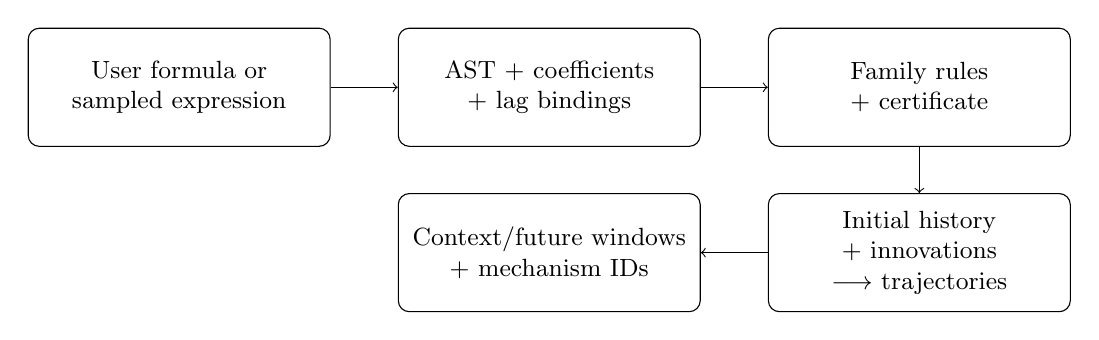
\begin{tikzpicture}[box/.style={draw,rounded corners,align=center,
    text width=3.6cm,minimum height=1.5cm,font=\small}]
\node[box] (tree) at (0,0) {User formula or\\sampled expression};
\node[box] (bound) at (4.7,0) {AST + coefficients\\+ lag bindings};
\node[box] (family) at (9.4,0) {Family rules\\+ certificate};
\node[box] (paths) at (9.4,-2.1) {Initial history\\+ innovations\\$\longrightarrow$ trajectories};
\node[box] (batch) at (4.7,-2.1) {Context/future windows\\+ mechanism IDs};
\draw[->] (tree) -- (bound);
\draw[->] (bound) -- (family);
\draw[->] (family) -- (paths);
\draw[->] (paths) -- (batch);
\end{tikzpicture}
\caption{Implemented generation stages. The selected family determines the
admissible expressions, initialization, and innovation law. The mechanism
record is retained alongside the observations.}
\label{fig:implemented-generator-pipeline}
\end{figure}

\subsubsection{Random Tree Sampling}
Within the selected vocabulary in Section~\ref{sec:generator-vocabulary},
the base sampler draws a binary-operator count, labels leaves as parameters
or lagged series, and recursively constructs the tree. Its implementation
is in \path{src/tsfmxai/generators/random_expression.py}.
For a subtree containing $o$ binary operators, the
probability of assigning $a$ operators to the left child is proportional to
the number of left shapes times the number of right shapes. These counts
are Catalan numbers. This produces a uniform distribution over ordered full
binary shapes conditional on $o$. Internal nodes
are labelled addition or multiplication. Zero-operator trees consist of one
leaf; required leaf types must fit the requested size.

The current random base grammar therefore uses binary operations; the
Shao--Wu transformation in Section~\ref{sec:implemented-shao-wu}
adds unary \texttt{Tanh} nodes to the same AST
representation. The wider unary--binary grammar in D'Ascoli et al.
provides the precedent. Our operator probabilities, parameter ranges, forced
lag presence, and multivariate source indices define the project's sampling
prior. Slot names are assigned in preorder, preserving the sampled left and
right children. This keeps numerical bindings and serialization reproducible
for a fixed seed.

\subsubsection{User-Provided Equations}
A researcher can specify the expression structure and its bindings directly
within the vocabulary in Section~\ref{sec:generator-vocabulary}. For example,
the skeleton $P_0x_0(t-L_0)+P_1$ becomes
$0.7x_0(t-2)+0.01$ after binding its slots. Numerical parameters and lag
assignments are retained with the AST so the resulting formula is executable
and can be inspected independently of its generated observations.
The selected family then applies its construction and admissibility rules
as described in Section~\ref{sec:generator-stability}; the resulting,
possibly transformed equation is the mechanism used for execution and
ground-truth extraction.

\subsection{Trajectory Generation}
\label{sec:generator-trajectories}

\subsubsection{Initial Histories and Random Innovations}
The initial history supplies the observations required by every lag leaf.
The AST represents the deterministic update; the executor adds the
innovation specified by the mechanism's noise law. These choices are retained
with the equation, and each generation family declares its own initialization
and innovation policies in Section~\ref{sec:generator-stability}.
The initial lag values and recursively generated observations have distinct
roles: the history is the starting state, and context/future windows select
their observations from the generated portion of the returned trajectory.

\subsubsection{Synchronous Multivariate Updates}
At target time $t$, a lag leaf reads $x_{j,t-\ell}$ with $\ell\geq1$.
Equivalently, from the common origin $\tau$, the first generated target uses
$t=\tau+1$. The shared executor
\path{src/tsfmxai/generators/stochastic.py} evaluates every target against the
same previous multivariate history, adds the supplied innovation, and then
appends all new values together. This synchronous update preserves the
intended lag relationships between channels. Model inputs and future targets
can subsequently be separated without changing the recorded equation.

\subsubsection{Multiple Trajectories from One Mechanism}
The equation structure, bound coefficients, and lag assignments stay fixed
while repeated trajectories receive separate initialization and innovation
streams. This distinguishes variation within one mechanism from variation
between sampled equations. The mechanism identifier connects those
trajectories to their shared equation and generation policy. Its executed
AST is also the source for the explanation references developed in
Section~\ref{sec:ground-truth-generation}.

\subsection{Reproducible and Parallel Generation}
\label{sec:generator-parallel}

\subsubsection{Seeds and Independent Random Streams}
Seeds are derived from the root seed and explicit job, attempt, and stream
indices. Local random-number generators isolate these draws from the
caller's global random state. Separate streams identify the mechanism,
initialization, and innovations; changing the number of workers preserves
the indexed draws and their final ordering. Worker-count and seed
independence are tested in the test suite.

\subsubsection{Parallel Jobs and Batch Construction}
The existing batch builder assigns one mechanism and several trajectories to
each job, then assembles windows with a requested minimum number of distinct
skeletons. It is implemented in
\path{src/tsfmxai/datasets/parallel_batch.py}. Ordering is restored when jobs
finish. This batch builder currently uses the original sampler with acceptance
checks; the four-family diagnostic comparison in
Section~\ref{sec:generator-evaluation-protocol} evaluates every attempted
mechanism and records failures. The generator policies and the empirical
comparison therefore retain their respective acceptance and accounting rules.

\subsection{Generation Overview}
\label{sec:generation-overview}

A mechanism is the equation executed at every generated step. Its structure,
coefficients, and lag assignments remain fixed while the initial history and
innovation sequence determine a particular trajectory. The same final equation,
initial history, and numerical innovations produce the same trajectory, up to
floating-point effects. A construction method can change that equation before
execution. The original and transformed equations must therefore be retained
separately, with ground-truth explanations referring to the executed mechanism.

Tables~\ref{tab:generation-overview-linear} and~\ref{tab:generation-overview-nonlinear}
show nine sampled examples, selected under restricted sampling configurations
to make these changes readable. The first column gives the original recurrence;
the middle columns give the recurrence produced by each construction; the last
column explains the feature being illustrated. The cases cover individual lags,
an offset, multiple memory scales, repeated factors, and nonlinear interactions.
They are worked examples rather than estimates of how often those structures
occur under the benchmark's full sampling prior.

\paragraph{Reading the equations and the innovations.}
To keep the tables compact, write $z_\ell=x_{t-\ell}$ and
$T_\ell=\tanh(z_\ell)$. A squared lag is displayed as $z_1^2$; its AST contains
two lag leaves joined by multiplication. The index $t$ is the current generated
step, so the first update after history ending at time zero uses $t=1$.
Every recurrence explicitly includes a fresh additive innovation, identified
by its superscript: O denotes the original AST, J the Jacobian method,
F factor saturation, P product-output saturation, and H Heaps. This term is
the generator's random innovation; forecast errors are measured later by
comparing predictions with generated observations.

Here the configured standard deviation is $\sigma_\varepsilon=0.05$.
The O, F, P, and H policies use i.i.d. Gaussian innovations with distribution
$\mathcal N(0,0.05^2)$. The J policy uses i.i.d. uniform innovations on
$[-\sqrt{3}(0.05),\sqrt{3}(0.05)]$ to respect its finite noise bound while
matching that standard deviation. These method labels identify policies;
actual noise sequences may be shared or independently drawn according to the
comparison protocol. Matching standard deviations alone leaves different noise
laws. A trajectory comparison must also specify its initial history and which
numerical innovations are shared. The constructors scale only the deterministic
expression; the innovation is added afterwards at every step.

\paragraph{Construction settings used in the tables.}
The Jacobian calculation uses $r_D=1$, $q_w=1.25$, target gain 0.9, and safety
multiplier 0.95. It scales the complete AST to meet both the sensitivity and
domain-containment checks of Section~\ref{sec:implemented-domain-contraction}.
The two Shao--Wu-inspired modes use target gain 0.8 and safety multiplier 0.95.
Factor saturation replaces lag leaves inside nonlinear products by their
hyperbolic tangents, then checks global sensitivity using the condition of
\citet[Theorem~5.1]{shao2007spectral}. Product-output saturation bounds each
complete nonlinear product and checks the project's second-moment envelope,
as detailed in Section~\ref{sec:implemented-shao-wu}. Their verification records
therefore certify different properties. Both preserve standalone linear terms
before applying their root multiplier. Even a candidate already within a
target bound receives the implementation's 0.95 safety multiplier.

\paragraph{How the Heaps column is matched to a linear example.}
Heaps constructs a linear VAR from free parameter matrices and an innovation
covariance \citep[Sections~2.1--2.2 and Appendix]{heaps2023stationarity}.
For this illustration, each scalar coefficient in the original linear formula
is supplied as the corresponding one-by-one free matrix $\mathbf U_\ell$;
missing lags receive zero. This is an explicit comparison convention, with
the same numerical entries interpreted in different parameter spaces.
The constructor then reconstructs the final AR coefficients jointly. We choose
its stationary mean to preserve the original intercept: after reconstruction,
divide that intercept by one minus the sum of the final AR coefficients.
With one lag, free entry 2 consequently produces coefficient
$2/\sqrt{5}\approx0.894427$. In R4, the free entries at lags 1 and 3 also
produce a coefficient at lag 2. Nonlinear rows indicate the linear scope of
this constructor. Section~\ref{sec:implemented-heaps} explains its standard
stationary-history sampling; the equations below describe the transition rule
separately from that initialization choice.

\paragraph{Reproduction and interpretation.}
The input equations are actual outputs of
\path{src/tsfmxai/generators/random_expression.py}, with the seeds shown in the
tables. Their configurations use one series, no time terminals, and no automatic
lag-coefficient gates; selected parameter magnitudes are fixed at 0.5 or 2 to
keep the arithmetic readable. Operator counts, sampling weights, and lag ranges
for each case are recorded in \path{scripts/check_generation_overview.py}.
Running \texttt{python} \path{scripts/check_generation_overview.py} reconstructs the
nine samples, checks all 27 AST transformations and five matched Heaps
constructions, and verifies the formulas numerically. Coefficients shown with
$\approx$ are rounded to six decimals; calculations retain full precision.
These examples compare construction rules. Explosion rates, initialization
effects, and generation speed require the separate trajectory experiments.

\begin{landscape}
\begingroup
\renewcommand{\baselinestretch}{1}
\footnotesize
\setlength{\tabcolsep}{3pt}
\setlength{\LTcapwidth}{.97\linewidth}
\renewcommand{\arraystretch}{1.2}
\begin{longtable}{@{}
>{\raggedright\arraybackslash}p{.13\linewidth}
>{\raggedright\arraybackslash}p{.14\linewidth}
>{\raggedright\arraybackslash}p{.15\linewidth}
>{\raggedright\arraybackslash}p{.17\linewidth}
>{\raggedright\arraybackslash}p{.17\linewidth}
>{\raggedright\arraybackslash}p{.19\linewidth}@{}}
\caption{Generation Overview: linear and affine sampled recurrences. Each cell
includes the innovation added at step $t$. The Heaps column uses the explicitly
declared free-parameter convention.}\label{tab:generation-overview-linear}\\
\toprule
Sampled equation / original AST & Jacobian: scaled AST & Shao--Wu: factors & Shao--Wu: product output & Heaps: linear construction & Why this example?\\
\midrule
\endfirsthead
\toprule
Sampled equation / original AST & Jacobian: scaled AST & Shao--Wu: factors & Shao--Wu: product output & Heaps: linear construction & Why this example?\\
\midrule
\endhead
\textbf{Operation}\newline
Keep the sampled formula and add the innovation at each step. &
Scale the complete deterministic expression to meet contraction and domain
bounds. In R2, multiply by $0.4275$. &
Apply $\tanh$ to lag factors inside nonlinear products, then scale the whole
expression to limit sensitivity. In R2, multiply by $0.38$. &
Apply $\tanh$ after the complete nonlinear product, then scale the whole
expression to satisfy the second-moment bound. &
Map free parameters to stable AR coefficients. For AR(1),
$a=u/\sqrt{1+u^2}$; $u=2$ gives $a\approx0.894427$. &
Each following row applies these operations to one input equation.
The innovation is added after the deterministic transformation.\\
\midrule
\textbf{R1; seed 0}\newline
$x_t=z_1+\varepsilon_t^{(\mathrm O)}$ &
$x_t=0.855z_1$\newline $+\varepsilon_t^{(\mathrm J)}$ &
$x_t=0.76z_1$\newline $+\varepsilon_t^{(\mathrm F)}$ &
$x_t=0.76z_1$\newline $+\varepsilon_t^{(\mathrm P)}$ &
$x_t\approx0.707107z_1$\newline $+\varepsilon_t^{(\mathrm H)}$ &
Unit feedback: the original is a random walk. All three constructions change
its memory strength.\\
\addlinespace
\textbf{R2; seed 0}\newline
$x_t=2z_1+\varepsilon_t^{(\mathrm O)}$ &
$x_t=0.855z_1$\newline $+\varepsilon_t^{(\mathrm J)}$ &
$x_t=0.76z_1$\newline $+\varepsilon_t^{(\mathrm F)}$ &
$x_t=0.76z_1$\newline $+\varepsilon_t^{(\mathrm P)}$ &
$x_t\approx0.894427z_1$\newline $+\varepsilon_t^{(\mathrm H)}$ &
Amplifying feedback. Scaling maps R1 and R2 to identical J/F/P drifts, while
the Heaps parameter map retains a difference.\\
\addlinespace
\textbf{R3; seed 2}\newline
$x_t=z_1-0.5$\newline $+\varepsilon_t^{(\mathrm O)}$ &
$x_t\approx0.578485$\newline $\times(z_1-0.5)$\newline $+\varepsilon_t^{(\mathrm J)}$ &
$x_t=0.76(z_1-0.5)$\newline $+\varepsilon_t^{(\mathrm F)}$ &
$x_t=0.76(z_1-0.5)$\newline $+\varepsilon_t^{(\mathrm P)}$ &
$x_t\approx0.707107z_1$\newline $-0.5+\varepsilon_t^{(\mathrm H)}$ &
Offset: the AST root multiplier scales the intercept too. J reserves space
for offset and noise; H preserves the intercept by the stated convention.\\
\addlinespace
\textbf{R4; seed 0}\newline
$x_t=z_1+z_3$\newline $+\varepsilon_t^{(\mathrm O)}$ &
$x_t\approx0.333659$\newline $\times(z_1+z_3)$\newline $+\varepsilon_t^{(\mathrm J)}$ &
$x_t=0.38(z_1+z_3)$\newline $+\varepsilon_t^{(\mathrm F)}$ &
$x_t=0.38(z_1+z_3)$\newline $+\varepsilon_t^{(\mathrm P)}$ &
$x_t\approx0.707107z_1$\newline $-0.5z_2+0.707107z_3$\newline $+\varepsilon_t^{(\mathrm H)}$ &
Separated lags: J weights older memory more strongly. Joint H reconstruction
introduces a lag-2 coefficient.\\
\addlinespace
\textbf{R5; seed 0}\newline
$x_t=z_{12}+\varepsilon_t^{(\mathrm O)}$ &
$x_t\approx0.073444z_{12}$\newline $+\varepsilon_t^{(\mathrm J)}$ &
$x_t=0.76z_{12}$\newline $+\varepsilon_t^{(\mathrm F)}$ &
$x_t=0.76z_{12}$\newline $+\varepsilon_t^{(\mathrm P)}$ &
$x_t\approx0.707107z_{12}$\newline $+\varepsilon_t^{(\mathrm H)}$ &
Long delay: the J weight $1.25^{11}$ requires substantially more attenuation
than in R1. Formula size alone misses this difficulty.\\
\bottomrule
\end{longtable}
\endgroup
\end{landscape}

\begin{landscape}
\begingroup
\renewcommand{\baselinestretch}{1}
\footnotesize
\setlength{\tabcolsep}{3pt}
\setlength{\LTcapwidth}{.97\linewidth}
\renewcommand{\arraystretch}{1.2}
\begin{longtable}{@{}
>{\raggedright\arraybackslash}p{.13\linewidth}
>{\raggedright\arraybackslash}p{.14\linewidth}
>{\raggedright\arraybackslash}p{.15\linewidth}
>{\raggedright\arraybackslash}p{.17\linewidth}
>{\raggedright\arraybackslash}p{.17\linewidth}
>{\raggedright\arraybackslash}p{.19\linewidth}@{}}
\caption{Generation Overview: nonlinear sampled recurrences.
Here $z_\ell=x_{t-\ell}$ and $T_\ell=\tanh(z_\ell)$.
Factor mode verifies global sensitivity; product-output mode verifies a
second-moment bound.}\label{tab:generation-overview-nonlinear}\\
\toprule
Sampled equation / original AST & Jacobian: scaled AST & Shao--Wu: factors & Shao--Wu: product output & Heaps: linear construction & Why this example?\\
\midrule
\endfirsthead
\toprule
Sampled equation / original AST & Jacobian: scaled AST & Shao--Wu: factors & Shao--Wu: product output & Heaps: linear construction & Why this example?\\
\midrule
\endhead
\textbf{Operation}\newline
Keep the sampled formula and add the innovation at each step. &
Scale the complete deterministic expression to meet contraction and domain
bounds. In R2, multiply by $0.4275$. &
Apply $\tanh$ to lag factors inside nonlinear products, then scale the whole
expression to limit sensitivity. In R2, multiply by $0.38$. &
Apply $\tanh$ after the complete nonlinear product, then scale the whole
expression to satisfy the second-moment bound. &
Map free parameters to stable AR coefficients. For AR(1),
$a=u/\sqrt{1+u^2}$; $u=2$ gives $a\approx0.894427$. &
Each following row applies these operations to one input equation.
The innovation is added after the deterministic transformation.\\
\midrule
\textbf{R6; seed 0}\newline
$x_t=z_1z_2+\varepsilon_t^{(\mathrm O)}$ &
$x_t=0.38z_1z_2$\newline $+\varepsilon_t^{(\mathrm J)}$ &
$x_t=0.38T_1T_2$\newline $+\varepsilon_t^{(\mathrm F)}$ &
$x_t=0.95\tanh(z_1z_2)$\newline $+\varepsilon_t^{(\mathrm P)}$ &
Outside the linear VAR vocabulary. &
Two distinct lag factors: contrast a scaled polynomial, bounded factors,
and a bounded complete product.\\
\addlinespace
\textbf{R7; seed 0}\newline
$x_t=z_1^2+\varepsilon_t^{(\mathrm O)}$ &
$x_t=0.4275z_1^2$\newline $+\varepsilon_t^{(\mathrm J)}$ &
$x_t=0.38T_1^2$\newline $+\varepsilon_t^{(\mathrm F)}$ &
$x_t=0.95\tanh(z_1^2)$\newline $+\varepsilon_t^{(\mathrm P)}$ &
Outside the linear VAR vocabulary. &
Repeated coordinate: two leaves refer to one lag. The conservative
derivative bound counts both occurrences.\\
\addlinespace
\textbf{R8; seed 5}\newline
$x_t=z_1^2z_2z_3$\newline $+\varepsilon_t^{(\mathrm O)}$ &
$x_t\approx0.177662$\newline $\times z_1^2z_2z_3$\newline $+\varepsilon_t^{(\mathrm J)}$ &
$x_t=0.19T_1^2T_2T_3$\newline $+\varepsilon_t^{(\mathrm F)}$ &
$x_t=0.95$\newline $\times\tanh(z_1^2z_2z_3)$\newline $+\varepsilon_t^{(\mathrm P)}$ &
Outside the linear VAR vocabulary. &
Four factors: increasing product degree raises the sensitivity budget.
P saturates the entire connected product once.\\
\addlinespace
\textbf{R9; seed 1438}\newline
$x_t=0.5z_1+z_1z_2$\newline $+\varepsilon_t^{(\mathrm O)}$ &
$x_t\approx0.310909$\newline $\times(0.5z_1+z_1z_2)$\newline $+\varepsilon_t^{(\mathrm J)}$ &
$x_t=0.304$\newline $\times(0.5z_1+T_1T_2)$\newline $+\varepsilon_t^{(\mathrm F)}$ &
$x_t=0.95$\newline $\times[0.5z_1+\tanh(z_1z_2)]$\newline $+\varepsilon_t^{(\mathrm P)}$ &
Outside the linear VAR vocabulary. &
Mixed linear and nonlinear feedback: selective saturation preserves the
linear lag; the root multiplier still scales both terms.\\
\bottomrule
\end{longtable}
\endgroup
\end{landscape}


% Retained writing notes for later expansion of this chapter:
% - Document accepted formula syntax, parser validation, and user-facing help.
% - Add a hand-computed indexing example and the context/future array layout.
% - Illustrate text, AST, infix formula, and serialization together.
% - Detail the frontend and mechanism-by-column/trajectory-by-row plots when
%   stable report figures are selected.
% - Expand batching/API coverage when the controlled families are integrated;
%   document DataLoader integration once implemented.
% - Keep mathematical admissibility in Chapter~\ref{sec:generator-stability}
%   and measured generator comparisons in Chapter~\ref{sec:results-discussion}.

\clearpage
\section{Stability and Quality Control of Generated Series}
\label{sec:generator-stability}

The shared AST representation can express mechanisms with very different
feedback and amplitude behaviour. This chapter defines the properties sought,
the diagnostics used to assess generated paths, and the controlled generation
policies. Each method presents its mathematical conditions before explaining
how the implementation checks them. The original AST supplies the reference;
bounded-domain contraction, nonlinear product saturation, and stationary VAR
construction impose different restrictions. Their measured trade-offs are
reported in Section~\ref{sec:implemented-generator-results}.

\subsection{Desired Mathematical Properties}
\label{sec:generator-properties}

The mathematical distinctions reviewed in
Section~\ref{sec:explosion-treatment} guide the construction and interpretation
of the generator families. A verification record states the property checked
for a mechanism together with its domain, innovation law, and initialization
assumptions.

\subsubsection{Amplitude and Moment Bounds}
An invariant bounded domain controls every trajectory for every allowed
innovation sequence. A uniform second-moment bound instead controls the
expected squared magnitude across repeated realizations, uniformly over
generated time. Gaussian innovations have unbounded support, so a process
with finite controlled moments can still cross a finite amplitude threshold.
The threshold-crossing diagnostic in Section~\ref{sec:generator-diagnostics}
therefore records finite-path events separately from the mathematical
property certified by the constructor.

\subsubsection{Contraction and Forgetting Initial Conditions}
Contraction compares two histories passed through the same update rule and
the same sampled innovation values at each future step. A geometric decrease
in their distance, or its specified moment, describes how the influence of
their initial histories disappears. Fresh innovations continue to drive the
process. The bounded-domain method and Shao--Wu factor mode verify this
property under their respective conditions in
Sections~\ref{sec:implemented-domain-contraction}
and~\ref{sec:implemented-shao-wu}.

\subsubsection{Stationarity and Initialization}
Strict stationarity means that the joint probability laws of a process are
unchanged by time shifts. A recurrence can admit a stationary solution while
a finite simulation starts from a separately chosen history distribution.
The uniform histories used by the AST families can consequently produce
initialization transients. The Heaps constructor instead draws the whole
initial lag history jointly from the stationary Gaussian law, as explained
in Section~\ref{sec:implemented-heaps}. Initialization, contraction, and
amplitude control are thus recorded as distinct properties of each policy.

\subsection{Common Diagnostics}
\label{sec:generator-diagnostics}

Unrestricted feedback can amplify observations over repeated execution.
A pretraining prior dominated by such behaviour would allocate much
of its capacity to rapidly growing recurrences. For the intended benchmark,
explosive cases can instead form an explicitly controlled difficulty group,
alongside mechanisms producing sustained variation at usable scales.

This section defines explosion, low-amplitude, and tail-flattening diagnostics.
The experiment configuration and timing protocol are specified in
Section~\ref{sec:generator-evaluation-protocol}. Their measured trade-offs
appear in Section~\ref{sec:implemented-generator-results}, where improved
growth control is weighed against reduced variation and computational cost.

\subsubsection{Explosion Detection}

The evaluator constructs the history according to each family, generates one
path up to the largest horizon, and reuses its prefixes. No generated prefix
is discarded before these observations: the original, bounded-domain, and
Shao--Wu families draw their initial histories directly, while Heaps draws
from its joint stationary law. It stops at the first
non-finite value or magnitude greater than 100, retaining that failing value.
The event remains counted at every later horizon, including a failure at the
last requested step. Every attempted mechanism stays in the denominator.
For multivariate use, any failing channel flags the system. These rules are
implemented in \path{src/tsfmxai/evaluation/stability.py} and
\path{src/tsfmxai/evaluation/generator_tradeoff.py}.

An amplitude threshold is an operational safeguard: Gaussian innovations have
unbounded support and can cross any finite threshold even under a stationary
law. The evaluator records finite threshold crossings separately from
non-finite outputs.

\subsubsection{Near-Zero Amplitude}
A completed, non-explosive prefix receives this label when every channel's
last 24 values lie in $[-0.15,0.15]$. The tolerance is three times the
innovation standard deviation used in this experiment, $\sigma_\varepsilon=0.05$.
Thus the label measures occupation of a small band during a finite window.
It can also be produced by a stationary process fluctuating near zero from
the beginning. Convergence of a trajectory to zero is a stronger,
infinite-time property requiring separate evidence.

\subsubsection{Nearly Constant Tails}
To capture stabilization around levels other than zero, let
$\bar x^{\mathrm{tail}}_{k,h}$ be the mean of channel $k$ over the last
$w_{\mathrm{tail}}$ generated observations at horizon $h$. Define
\begin{equation}
 V_h^{\mathrm{tail}}=
 \max_k\max_{h-w_{\mathrm{tail}}<v\leq h}
 \left|x_{k,\tau+v}-\bar x^{\mathrm{tail}}_{k,h}\right|.
 \label{eq:generator-flat-tail}
\end{equation}
A completed, non-explosive prefix is nearly constant when
$V_h^{\mathrm{tail}}\leq\delta_{\mathrm{flat}}$. The implementation uses
$w_{\mathrm{tail}}=24$ and the operational tolerance
$\delta_{\mathrm{flat}}=3\sigma_\varepsilon=0.15$, retaining each channel's
mean and variation. Persistence requires both consecutive terminal windows
to pass, and all 48 terminal observations to satisfy the same tolerance
around their pooled channelwise mean. This joint check captures level changes
between individually flat windows. Variation is measured on signed channels
before taking a maximum across channels.

The first 24 generated observations, after the family's initialization,
provide a disjoint reference window. Observed flattening requires persistent
flatness, at least one channel initially above the variation tolerance, and
a reduction of at least 50\% in every such channel. The reduction compares
the pooled 48-step terminal variation with the initial 24-step variation.
Quiet initial and terminal windows are recorded separately; intermediate
behaviour remains unrestricted. A persistent flat tail is labelled away
from zero when at least one channel's final mean lies outside $[-0.15,0.15]$.

Amplitude decline towards the near-zero band uses absolute values relative
to zero: every channel must remain in the band for the final 48 steps,
at least one channel must initially exceed the band, and every such channel
must reduce its maximum absolute value by at least 50\%. These finite-window
labels can overlap. All rates retain every attempted trajectory in the
denominator; exploded prefixes are ineligible for tail measurements.
The notebook also reports eligible-only rates and sensitivity to
$\delta_{\mathrm{flat}}\in\{\sigma_\varepsilon,2\sigma_\varepsilon,
3\sigma_\varepsilon\}$. These thresholds and the reduction factor are
configurable project choices. The implementation is in
\path{src/tsfmxai/evaluation/tail_behavior.py}.

\subsection{Original AST Generator as the Reference}
\label{sec:implemented-original-baseline}

The reference uses the expression sampler described in
Section~\ref{sec:generator-expression-pipeline}, with the comparison settings
in Section~\ref{sec:generator-evaluation-protocol}.
It executes the sampled sums and products of lagged values directly,
starting from a uniform history in $[-1,1]$ and adding Gaussian innovations
with standard deviation 0.05. Its sampled coefficients remain unchanged.
Every attempted mechanism enters the evaluation, including trajectories
that trigger the stopping rule. This supplies the reference rates of
explosion and low amplitude, and the generation cost against which the
three controlled constructions below are compared.

\subsection{Jacobian-Based Contraction on an Invariant Domain}
\label{sec:implemented-domain-contraction}

\subsubsection{Pipeline Overview}
The starting point is a randomly sampled equation that uses past observations
to generate the next value. We adjust its coefficients so that it can be
repeated safely within a chosen range. The pipeline is:
\begin{enumerate}
\item \textbf{Sample the equation.} Generate an AST with lagged inputs and
coefficients, preserving an explicit formula for the mechanism.
\item \textbf{Choose the allowed range and noise.} Specify where all initial
values may lie and the largest innovation that may be added at each step.
\item \textbf{Bound the output and its sensitivity.} Calculate conservative
limits on the equation's magnitude and on how changes in its historical
inputs affect the next state, including the copied lag values.
\item \textbf{Scale and verify the equation.} Reduce its overall strength
until the generated values remain in the allowed range and differences
between histories shrink under shared future noise.
\item \textbf{Generate trajectories.} Draw initial values inside that range
and execute the adjusted equation with bounded random innovations.
\item \textbf{Check the implementation empirically.} Simulate several
trajectories and check that their values and measured sensitivities respect
the calculated limits.
\end{enumerate}
Steps 3--4 establish the sufficient mathematical conditions; Step 6 tests
whether the implementation behaves consistently with them. The following
steps explain both the calculation and its purpose.

\subsubsection{Steps 1--2: Sample the Equation and Define Its Allowed Inputs}
This method controls the feedback created when generated values become inputs
to later steps. We want two properties: every observation stays inside a
chosen interval, and differences caused by the initial history shrink over
time. To examine the second property, run the same equation from two different
histories and give both runs exactly the same sampled noise value at each
future step. Their remaining difference then reflects the effect of the
initial histories. Fresh noise can keep both series fluctuating.

The sampler in \path{src/tsfmxai/generators/contraction.py} generates a
sum/product AST and attaches coefficients to its lag leaves. We choose
an allowed interval $[-r_D,r_D]$ and a noise bound $b_\varepsilon<r_D$.
Every initial lag value must belong to that interval. These choices define
where the equation will be checked and reserve room for the innovations.

\paragraph{Store the values needed for the next update.}
Consider the two-lag example
\begin{equation}
 x_{t+1}=0.2x_t+0.1x_tx_{t-1}+\varepsilon_{t+1},
 \qquad F_{\mathcal T}(s_0,s_1)=0.2s_0+0.1s_0s_1.
 \label{eq:jacobian-explanatory-recurrence}
\end{equation}
The function $F_{\mathcal T}$ is the deterministic part of the equation;
$\varepsilon_{t+1}$ is the random innovation added at that step.
The next value requires both $x_t$ and $x_{t-1}$, so store them together as
$\mathbf{s}_t=(x_t,x_{t-1})^\top$. This vector is called the \emph{state}:
it contains the complete history needed for one update. Its first coordinate,
$s_0$, is the newest value; $s_1$ is the preceding value.

After generating $x_{t+1}$, the new state is $(x_{t+1},x_t)^\top$:
insert the new value, move the previous newest value one position back, and
discard the oldest value. When the largest lag is $L$, the state stores the
$L$ most recent observations, and this complete update is
\begin{equation}
 \mathcal F_\varepsilon(\mathbf{s})=
 \bigl(F_{\mathcal T}(\mathbf{s})+\varepsilon,
       s_0,\ldots,s_{L-2}\bigr)^\top.
 \label{eq:implemented-state-transition}
\end{equation}
Thus $\mathcal F_\varepsilon$ describes both the equation and its memory
update. Stacking lagged observations this way is the \emph{augmented-state}
representation discussed by \citet{laraba2016setinvariance}.

\subsubsection{Step 3: Bound the Output and the Sensitivity of the Whole State}
\paragraph{Use derivatives to measure sensitivity to that history.}
A partial derivative measures how an output changes when one input changes
slightly while the other inputs stay fixed. The \emph{Jacobian} collects
these derivatives for every output coordinate of the state update.
For the example above,
\begin{equation}
 J_{\mathcal F}(\mathbf{s})=
 \begin{pmatrix}
  \partial F_{\mathcal T}/\partial s_0 &
  \partial F_{\mathcal T}/\partial s_1\\
  1 & 0
 \end{pmatrix}
 =\begin{pmatrix}
   0.2+0.1s_1 & 0.1s_0\\
   1 & 0
  \end{pmatrix}.
 \label{eq:jacobian-explanatory-matrix}
\end{equation}
The first row measures the sensitivity of the newly generated value.
The second row describes memory: the previous newest value is copied with
multiplier one. The additive noise has derivative zero with respect to the
history. In the two-run comparison its value is shared, so it also cancels
when subtracting the two updates.

\paragraph{Evaluate the bounds over every allowed history.}
Choose a radius $r_D>0$ and require every stored value to lie in
$[-r_D,r_D]$. The set of all allowed histories is
$D=[-r_D,r_D]^L$, called a \emph{box}. With two lags and $r_D=1$, it contains
every pair $(s_0,s_1)$ whose coordinates are between $-1$ and $1$.
Write $\overline d_d$ for an upper bound on the magnitude of the derivative
with respect to coordinate $s_d$. On this box, the example's bounds are
$\overline d_0=0.3$ and $\overline d_1=0.1$.
They cover every allowed history, rather than only the values visited by
sampled trajectories.

Derivatives initially describe small changes. To control a finite difference
between two histories, consider the straight line joining them. Every point
on that line remains inside a box; this property is called \emph{convexity}.
The derivative bound therefore applies along the entire line and bounds the
total output difference. The argument requires a continuously differentiable
update: the derivatives exist and vary continuously. The sampled sums and
products satisfy this smoothness requirement.

\paragraph{Measure changes in the whole state, including copied lags.}
For $L\geq2$, each memory-copy row has one entry equal to one. The ordinary
infinity norm takes the largest absolute row sum, so the augmented Jacobian
has norm at least one even when the recurrence eventually forgets its
history. To establish strict contraction at each update, we use weights
that account for information moving into older memory positions while
retaining its influence on new observations. Specifically, we use fixed
positive weights $w_d=q_w^d$, with $q_w>1$, and measure a state
difference $\Delta\mathbf{s}=\mathbf{s}-\mathbf{s}'$ by
\begin{equation}
 \|\Delta\mathbf{s}\|_{\mathbf w,\infty}
 =\max_{0\leq d<L}\frac{|s_d-s'_d|}{w_d}.
 \label{eq:jacobian-weighted-distance}
\end{equation}
In words, divide each coordinate difference by its weight and take the largest
result. This is the \emph{weighted infinity norm}; the same weights are used
at every step. For two lags with $q_w=1.25$, an unchanged difference copied
from the newest to the older position is divided by 1.25, giving a factor
of 0.8. At the same time, the older lag's sensitivity in the new-value row is
multiplied by 1.25, so its effect on future observations remains included.

Combining the new-value row and the memory-shift rows gives, for $L\geq2$,
\begin{equation}
 \sup_{\mathbf{s}\in D}\|J_{\mathcal F}(\mathbf{s})\|_{\mathbf w,\infty}
 \leq\max\left\{\sum_{d=0}^{L-1}\overline d_d q_w^d,
                       q_w^{-1}\right\}<1.
 \label{eq:implemented-weighted-contraction}
\end{equation}
Here $\sup$ means the worst case over all histories in the box, and the matrix
norm measures the largest amplification of the state difference in
Eq.~\eqref{eq:jacobian-weighted-distance}. The sum bounds the new-value row;
$q_w^{-1}$ bounds each copy into the next history position. For $L=1$,
only the new-value row exists. Call a verified common upper bound $\gamma<1$.
While both runs remain in $D$, one update reduces the measured distance by
a factor at most $\gamma$. Repeating this comparison for $v$ updates gives
\begin{equation}
 \|\mathbf{s}_{\tau+v}-\mathbf{s}'_{\tau+v}\|_{\mathbf w,\infty}
 \leq\gamma^v
       \|\mathbf{s}_{\tau}-\mathbf{s}'_{\tau}\|_{\mathbf w,\infty}.
 \label{eq:jacobian-history-forgetting}
\end{equation}
The distance decreases geometrically. For example, $\gamma=0.8$ limits it
after ten updates to $0.8^{10}\approx0.107$ times its initial value.
This is a guaranteed upper bound on the remaining distance; particular
trajectories can lose their dependence on the initial history faster.
Each coordinate difference is at most its fixed weight multiplied by this
measured distance. As the distance tends to zero, every individual
lag-coordinate difference therefore tends to zero as well. The weighting
changes how we measure the histories while leaving their generated values
unchanged.

\paragraph{Bound the output to keep subsequent states inside the checked box.}
The bound above remains useful only while the states stay inside $D$.
We therefore also require
$\mathcal F_\varepsilon(D)\subseteq D$ for every allowed innovation: starting
inside the box must produce another state inside it. This property is called
\emph{invariance}. With $|\varepsilon_t|\leq b_\varepsilon$, it is ensured by
\begin{equation}
 \sup_{\mathbf{s}\in D}|F_{\mathcal T}(\mathbf{s})|
       +b_\varepsilon\leq r_D.
 \label{eq:jacobian-domain-containment}
\end{equation}
The equation reserves enough room for both the deterministic output and the
largest allowed noise value. The copied lag values already belong to the
interval. Starting with a history in $D$, the same reasoning applies again
at every step: all observations stay bounded, and the sensitivity estimate
remains applicable.

\paragraph{Connection to the published theory.}
\citet[Definition~6 and Theorems~15--16]{tran2019convergence} develop the
relationship between contraction and \emph{incremental stability}, the
decrease of differences between trajectories. The fixed weighted norm and
box argument above are the project's sufficient construction for this
property. The state stacking and invariant-set viewpoint follow the concepts
reviewed by \citet{laraba2016setinvariance}. The conclusions here concern
histories inside the specified box and the specified bounded innovations.

\paragraph{Calculate conservative bounds from the AST.}
Starting at the leaves, the code records a possible value interval and
absolute derivative bounds for each subtree. Addition adds the bounds;
multiplication combines the intervals and uses the product rule for the
derivatives. For example, $s_0s_1$ lies in $[-1,1]$ when both inputs do, and
its derivatives are $s_1$ and $s_0$, each bounded in absolute value by one.
These calculations cover the full box. They can overestimate the actual
range, particularly when repeated leaves refer to the same coordinate.

\subsubsection{Step 4: Scale the Equation and Verify Both Conditions}
The constructor multiplies the complete expression by a calculated factor.
Reducing this factor decreases both the
deterministic output bound and the new-value row's derivative bounds. The
factor must leave room for the noise in
Eq.~\eqref{eq:jacobian-domain-containment} and meet the target gain in
Eq.~\eqref{eq:implemented-weighted-contraction}. The copied-lag gain depends
on $q_w$, so this weight parameter is chosen to meet the target as well.
The final expression retains the multiplier, making the executed equation
available for inspection and ground-truth extraction.

\paragraph{Worked example using the implemented rules.}
For Eq.~\eqref{eq:jacobian-explanatory-recurrence} on $[-1,1]^2$, the
unscaled deterministic magnitude is at most 0.3 and the derivative bounds
are $(0.3,0.1)$. The comparison settings use $q_w=1.25$, target gain 0.9,
and uniform innovations with
$b_\varepsilon=\sqrt{3}\,0.05\approx0.0866$. This uniform law has standard
deviation 0.05, matching the Gaussian noise scale in the other families.
These numerical settings are implementation choices within the admissible
conditions: the target 0.9 leaves a gap of 0.1 below the contraction threshold,
and $q_w=1.25$ gives a memory-copy gain of 0.8, below that target. The safety
multiplier 0.95 applies a further 5\% reduction to the allowed drift scale.
Both checks already pass; the constructor still applies its 0.95 safety
multiplier. The executed drift is therefore
$0.19s_0+0.095s_0s_1$. Its derivative bounds are $(0.285,0.095)$, giving
\begin{equation}
\begin{gathered}
 \gamma=\max\{0.285+1.25(0.095),\,0.8\}=0.8,
 \\
 0.285+\sqrt{3}(0.05)\approx0.3716<1.
\end{gathered}
 \label{eq:jacobian-worked-checks}
\end{equation}
Here the memory-copy row determines the final gain of 0.8; scaling the drift
reduces only the new-value row. The first check controls forgetting of the
initial history; the second
keeps the generated values inside $[-1,1]$. This is a hand-worked project
example, checked against the constructor in the test suite.

\paragraph{Retain the verification record.}
After scaling, the constructor checks the adjusted equation and stores the
domain, noise bound, derivative bounds, and resulting gain. These quantities
describe the equation that will actually be simulated. The implementation
uses floating-point calculations and a safety margin when evaluating the
bounds.

\paragraph{Effect on the sampled mechanisms.}
The scale changes the coefficients of the sampled equation and therefore
the dynamics represented in the benchmark. Older lags receive larger
multipliers in the sensitivity bound: with $q_w=1.25$, offset $d=11$
(lag 12) contributes with weight $1.25^{11}\approx11.64$. This can require
stronger attenuation of the whole expression. With the innovation scale
held fixed, that attenuation can weaken dependence on the history and
increase the relative influence of noise. These possible effects motivate
the amplitude and nearly constant-tail diagnostics in
Section~\ref{sec:generator-diagnostics}. The bound is a sufficient condition;
an expression exceeding it may still satisfy a different stability criterion.

\subsubsection{Step 5: Draw Initial Histories and Generate Trajectories}
The current constructor handles one series and excludes an explicit time
terminal. Its initial history is sampled uniformly inside the box; subsequent
observations are generated directly. Uniform innovations supply the finite
noise bound required for containment in the box.
The mathematical checks permit any fixed initial history inside the box;
uniform sampling is the current implementation's choice. A larger allowed
range requires recalculating the bounds and the scale. The trajectory
generator also checks that each newly generated value remains finite and
inside the certified interval.

\paragraph{Stationary law and initialization.}
For each fixed sampled mechanism, the contraction and bounded invariant
domain above, together with i.i.d. innovations, satisfy the conditions of
\citet[Theorem~1]{diaconis1999iterated} for a unique stationary distribution
of the lag state. The state distribution approaches this law from an
arbitrary initial history inside the box. Strict stationarity from the
start requires drawing the initial lag state jointly from that stationary
law, independently of future innovations. Our uniform history sampling can
instead produce an initialization transient, during which the distribution
changes as the process approaches its stationary law. As discussed in
Section~\ref{sec:generator-properties}, containment and forgetting still
hold throughout that transient.

\subsubsection{Step 6: Test the Implementation by Simulation}
Monte Carlo simulations exercise the generator using several sampled
histories and innovation sequences. They check whether generated values
remain inside the chosen interval and whether local Jacobian values respect
the verified gain. This can reveal an error in the bound calculation, lag
ordering, or trajectory execution. The mathematical guarantee comes from
the full-domain checks in Steps 3--4; the simulations provide an additional
implementation check. The common diagnostics in
Section~\ref{sec:generator-diagnostics} then measure explosions, low amplitude,
and nearly constant tails under the declared evaluation protocol.

\subsection{Shao--Wu-Inspired Nonlinear Generation}
\label{sec:implemented-shao-wu}

The generator offers two standard positions for the hyperbolic tangent:
\texttt{product\_lags} applies it to the lag factors before multiplication,
whereas \texttt{product\_output} applies it once after the complete product.
For two historical inputs $z_1,z_2$, these choices give
$\tanh(z_1)\tanh(z_2)$ and $\tanh(z_1z_2)$, respectively. A term containing
only a coefficient and one lag remains linear in both modes. The selected
mode is retained with the mechanism. Each mode carries a verification record
stating the particular property checked below.

\subsubsection{Desired Property and Shao--Wu's Theorem}
\label{sec:implemented-shao-wu-theory}
A generated series should retain useful stochastic variation while its
magnitudes remain controlled. We also seek a stronger property: the effect
of an arbitrarily supplied initial history should disappear. Imagine running
the same equation twice from different histories, then supplying exactly the
same sampled noise value to both runs at every future step. A decreasing
distance then measures the loss of dependence on their initial histories.

\citet[Section~3, Eq.~(3.1), electronic reprint p.~5]{shao2007spectral}
formalize this comparison as \emph{geometric moment contraction} (GMC).
For the second-moment version used here,
\begin{equation}
 \mathbb E\|\mathbf x_{\tau+v}-\mathbf x'_{\tau+v}\|_2^2
 \leq C_{\mathrm{GMC}}\rho_{\mathrm{GMC}}^{v},
 \qquad C_{\mathrm{GMC}}>0,\quad 0<\rho_{\mathrm{GMC}}<1.
 \label{eq:implemented-gmc-forgetting}
\end{equation}
The expectation averages squared distances across repeated noise
realizations. The upper bound decreases geometrically; individual
distances can fluctuate from step to step. In the paper's stationary
comparison the histories arise from independent past innovation sequences,
and the future innovation values are shared. Theorem~5.1 also supplies
forgetting bounds for fixed initial histories in its proof.

\paragraph{Theorem used for the factor mode.}
Let $\mathbf{s}_t=(\mathbf x_t,\ldots,\mathbf x_{t-L+1})$ store the $L$
historical vectors required for the next update, and write
\begin{equation}
 \mathbf x_{t+1}=\mathcal R_{\mathcal T}(\mathbf{s}_t;
                                      \boldsymbol\varepsilon_{t+1})
 =F_{\mathcal T}(\mathbf{s}_t)+\boldsymbol\varepsilon_{t+1}.
 \label{eq:implemented-gmc-recurrence}
\end{equation}
Here $F_{\mathcal T}$ is the deterministic expression executed by the AST.
We use the following specialization of
\citet[Theorem~5.1 and its proof, electronic reprint pp.~11--12]{shao2007spectral}
to second moments:
\begin{enumerate}
\item The update rule is measurable and fixed over time. Its innovations
are independent and identically distributed over time.
\item The next observation has a finite second moment at some fixed
reference history. We use the zero history:
$\|\mathcal R_{\mathcal T}(\mathbf0;\boldsymbol\varepsilon)\|_{L^2}<\infty$,
where $\|Z\|_{L^2}=(\mathbb E\|Z\|_2^2)^{1/2}$.
\item For every pair of possible histories, the same-innovation comparison
satisfies
\begin{equation}
\begin{split}
 \|\mathcal R_{\mathcal T}(\mathbf{s};\boldsymbol\varepsilon)
      -\mathcal R_{\mathcal T}(\mathbf{s}';\boldsymbol\varepsilon)\|_{L^2}
 &\leq\sum_{d=0}^{L-1}a_d^{\mathrm{GMC}}
                       \|\mathbf{s}_d-\mathbf{s}'_d\|_2,\\
 a_d^{\mathrm{GMC}}&\geq0,\qquad
 c_{\mathrm{GMC}}:=\sum_{d=0}^{L-1}a_d^{\mathrm{GMC}}<1.
\end{split}
\label{eq:implemented-gmc-condition}
\end{equation}
The vector $\mathbf{s}_d\in\mathbb R^N$ contains all channels at offset $d$.
Each $a_d^{\mathrm{GMC}}$ is a sensitivity budget for one historical vector;
their sum limits the combined feedback through all channels and lags.
\end{enumerate}
These conditions yield a causal strictly stationary solution with GMC:
present and past innovations determine the solution, and its joint
distributions are unchanged by time shifts. The finite histories supplied
to the simulator have their own declared distribution, so early generated
observations can show an initialization transient.

\subsubsection{Factor Saturation and Contraction Verification}
The implementation in \path{src/tsfmxai/generators/shao_wu.py}
samples a tree of sums and products with finite coefficients and positive
lags. It then performs the following checks.

\subparagraph{1. Saturate the factors that create nonlinear feedback.}
When a product combines two lag-dependent factors, its lag leaves receive
$\tanh$ before the product is evaluated. For example,
$a x_t x_{t-1}+b x_{t-2}$ becomes
$a\tanh(x_t)\tanh(x_{t-1})+b x_{t-2}$.
This controls the magnitudes of the nonlinear factors and their derivatives.
The last term keeps its linear dependence; its derivative is the finite
coefficient $b$. Every output uses fixed parameters and i.i.d. Gaussian
innovations with covariance $\sigma_\varepsilon^2 I$.

\subparagraph{2. Calculate conservative bounds along the AST.}
For each subtree $e$, let $A(e)$ bound its absolute value and let $D(e)$
contain nonnegative absolute derivative bounds by source and lag.
\begin{table}[H]
\centering\small
\begin{tabular}{@{}lll@{}}
\toprule
Subexpression & Amplitude bound $A$ & Derivative bounds $D$\\
\midrule
Constant $c$ & $|c|$ & $0$\\
Lag leaf & $+\infty$ & $1$ at its source/lag, $0$ elsewhere\\
$\tanh(e)$ & $1$ & $D(e)$\\
$e_1+e_2$ & $A(e_1)+A(e_2)$ & $D(e_1)+D(e_2)$\\
$e_1e_2$ & $A(e_1)A(e_2)$ & $A(e_2)D(e_1)+A(e_1)D(e_2)$\\
\bottomrule
\end{tabular}
\caption{Project rules for global size and derivative bounds. A zero
derivative contributes zero even when the other amplitude bound is infinite.
The $\tanh$ row uses $|\tanh'(z)|\leq1$ and can overestimate the true derivative.}
\label{tab:ast-global-bounds}
\end{table}
For a product, a perturbation in either factor is multiplied by the other
factor's magnitude; this is the product rule. Saturating the nonlinear
factors makes these upper bounds finite. A free linear term can have
unbounded amplitude and a finite derivative. The theorem uses the
derivative budgets and the moment at the reference history, so such terms
can remain in the factor-mode construction.

\subparagraph{3. Scale the combined sensitivity below one.}
For offset $d$, stack all target-by-source derivative bounds into an
$N\times N$ nonnegative matrix $\mathbf D_d$. Its largest singular value
bounds the amplification of a change in that whole historical vector.
Set
\begin{equation}
 \widetilde a_d=\|\mathbf D_d\|_2,\qquad
 \widetilde c=\sum_d\widetilde a_d,\qquad
 \eta_{\mathrm{GMC}}=
 \eta_{\mathrm{safe}}\min\{1,g_\star/\widetilde c\}.
 \label{eq:implemented-gmc-scaling}
\end{equation}
When $\widetilde c=0$, the minimum is defined as one. The defaults
$g_\star=0.8$ and $\eta_{\mathrm{safe}}=0.95$ give a final summed budget
$c_{\mathrm{GMC}}\leq0.76$. All output trees receive the same calculated
root multiplier, stored as \texttt{GMC\_SCALE}. It is computed after
sampling the structure and bindings. This changes the executed
coefficients while preserving the lag support.

Integrating the derivative bound along the line between two histories
gives Eq.~\eqref{eq:implemented-gmc-condition}. The additive innovation
cancels in that comparison because its numerical value is shared.
Using a whole matrix for each lag accounts for feedback between channels.

\subparagraph{4. Check the reference moment and retain the verification record.}
With the scaled drift $F_{\mathcal T}$, the Gaussian innovation law gives
\begin{equation}
 \|\mathcal R_{\mathcal T}(\mathbf0;\boldsymbol\varepsilon)\|_{L^2}
 =\left(\|F_{\mathcal T}(\mathbf0)\|_2^2+
                   N\sigma_\varepsilon^2\right)^{1/2}<\infty.
 \label{eq:implemented-gmc-anchor}
\end{equation}
Thus the theorem's reference-moment condition is checked directly even
when the drift is unbounded away from zero.
\texttt{ShaoWuCertificate} stores the lag budgets, their sum, the reference
moment, and the innovation moment. Its guarantee is identified as
\path{geometric_moment_contraction}.

For example, the proposed drift $0.3\tanh(x_t)\tanh(x_{t-1})$ has two
derivative bounds of $0.3$. Applying the default safety factor gives
\begin{equation}
 x_{t+1}=0.285\tanh(x_t)\tanh(x_{t-1})+\varepsilon_{t+1},
 \qquad \varepsilon_{t+1}\sim\mathcal N(0,0.05^2).
 \label{eq:implemented-gmc-example}
\end{equation}
The final total sensitivity bound is $0.57<1$ and the reference moment is
finite. This is a worked project construction using the cited theorem.

\subsubsection{Product-Output Saturation and Moment Bounds}
The second standard option evaluates the product first, then applies
$\tanh$ once. Its construction keeps history-independent multiplicative
coefficients outside the saturation: both $a(z_1z_2)$ and $(az_1)z_2$
therefore produce $a\tanh(z_1z_2)$. For three or more factors the entire
connected product is saturated once. Additive terms keep their original
roles.

This choice directly bounds the product's output. Its sensitivity has a
different behaviour:
\begin{equation}
 \frac{\partial\,\tanh(z_1z_2)}{\partial z_1}
 =z_2\bigl[1-\tanh^2(z_1z_2)\bigr].
 \label{eq:implemented-product-output-derivative}
\end{equation}
At $z_1=0$, this derivative equals $z_2$. Distinct lag coordinates can make
it arbitrarily large. Repeated occurrences of the same coordinate require
a separate calculation: $\tanh(z^2)$ has a bounded derivative.
Consequently, the conservative AST derivative test records what it can
verify; an infinite computed upper bound can represent overestimation.

The standard product-output mode checks a \emph{uniform second-moment
bound} by a separate project argument. Its growth envelope is
\begin{equation}
 \|F_{\mathcal T}(\mathbf{s})\|_2
 \leq B_{\mathrm{amp}}+
      \sum_{d=0}^{L-1} b_d^{\mathrm{amp}}\|\mathbf{s}_d\|_2,
 \qquad q_{\mathrm{amp}}:=\sum_d b_d^{\mathrm{amp}}<1.
 \label{eq:implemented-amplitude-envelope}
\end{equation}
Here $B_{\mathrm{amp}}$ covers constants and bounded nonlinear terms.
The nonnegative $b_d^{\mathrm{amp}}$ cover the magnitude of the remaining
unsaturated historical terms. They are \emph{growth coefficients}, whereas
$a_d^{\mathrm{GMC}}$ bound differences between histories.

To compute the envelope, a parameter contributes its absolute value to
the bounded part; a lag contributes one to its source/lag growth
coefficient; $\tanh(e)$ contributes a bounded part of one. Addition sums
these bounds. Multiplication by a bounded factor scales them. A product of
two unbounded envelopes is flagged for another construction. The mode
stacks the nonnegative growth coefficients into one target-by-source matrix
per lag and uses its largest singular value for $b_d^{\mathrm{amp}}$;
$B_{\mathrm{amp}}$ is the Euclidean norm of the componentwise bounded parts.
The mode
scales the complete drift using Eq.~\eqref{eq:implemented-gmc-scaling}
with the unscaled growth-coefficient sum in place of $\widetilde c$.
It stores the correspondingly scaled envelope for the executed equation.
Its root multiplier is stored as \texttt{AMPLITUDE\_SCALE}.

Let $M_0$ bound the $L^2$ norm of every initial lag vector. Minkowski's
inequality, the triangle inequality for root mean squared magnitudes, gives
\begin{equation}
 \|\mathbf x_{t+1}\|_{L^2}
 \leq B_{\mathrm{amp}}+
      \sum_d b_d^{\mathrm{amp}}\|\mathbf x_{t-d}\|_{L^2}
      +\sigma_\varepsilon\sqrt N.
 \label{eq:implemented-amplitude-recursion}
\end{equation}
Define
\begin{equation}
 M_{\mathrm{amp}}=
 \max\left\{M_0,\,
       \frac{B_{\mathrm{amp}}+\sigma_\varepsilon\sqrt N}
            {1-q_{\mathrm{amp}}}\right\}.
 \label{eq:implemented-amplitude-bound}
\end{equation}
If the historical vectors have $L^2$ norms at most $M_{\mathrm{amp}}$,
the next vector has norm at most
$B_{\mathrm{amp}}+q_{\mathrm{amp}}M_{\mathrm{amp}}
+\sigma_\varepsilon\sqrt N\leq M_{\mathrm{amp}}$.
Induction therefore yields
$\sup_{v\geq1}\mathbb E\|\mathbf x_{\tau+v}\|_2^2
\leq M_{\mathrm{amp}}^2$.
The uniform initial box gives the safe choice $M_0=r_0\sqrt N$.
The implementation stores these quantities in
\texttt{AmplitudeMoment\-Certificate}, with guarantee
\path{uniform_second_moment_bound}. This is our derived amplitude
criterion. Exponential forgetting and a stationary initialization require
their own additional conditions.

The pure saturated-product example
$x_{t+1}=\tanh(s_0s_1)+\varepsilon_{t+1}$ is particularly simple:
independent zero-mean Gaussian innovations give
$\mathbb E x_{t+1}^2\leq1+\sigma_\varepsilon^2$ at every generated step.
If two inputs are instead supplied by an already jointly stationary
external process, applying a fixed pointwise transformation preserves
their time-shift-invariant joint laws. In a feedback generator, the
history belongs to the newly defined recurrence, whose own growth or
contraction conditions must be checked as above.

For a scalar example
$F(\mathbf{s})=0.2s_0+0.4\tanh(s_0s_1)$, the growth coefficient is $0.2$
and the bounded part is $0.4$. The default multiplier is $0.95$, giving
$q_{\mathrm{amp}}=0.19$ and $B_{\mathrm{amp}}=0.38$.
With $r_0=1$ and $\sigma_\varepsilon=0.05$,
Eq.~\eqref{eq:implemented-amplitude-bound} gives $M_{\mathrm{amp}}=1$.
This example controls expected squared magnitude while allowing stochastic
fluctuations and sensitivity to the history.

\subsubsection{Initialization and Independent Innovations}
Both standard modes draw their initial $N\times L$ history directly from
$[-r_0,r_0]$, then generate the requested observations with independent
Gaussian innovations. The initial values are retained as a separate history
in the returned array; the subsequent entries are recursively generated.
A dataset window or diagnostic must select those generated entries explicitly.

The two standard transformations admit the configured sums/products through
their respective checks; a numerical verification failure is reported.
Legacy all-lag saturation and unsaturated sampling remain available for
reproducing earlier experiments. The unsaturated sampler rejects the entire
candidate mechanism when its conservative global derivative bound is
infinite, then samples a new skeleton, coefficients, and lags with a
deterministically derived attempt seed. This retry cost belongs to mechanism
sampling. A recorded zero-rejection rate for a standard mode describes the
chosen prior and execution.

Gaussian innovations have unbounded support. A finite amplitude threshold
can therefore be crossed even by a process with a uniform second-moment
bound or a stationary law. Tail flatness, low amplitude, and their observed
changes remain empirical diagnostics, as defined in
Section~\ref{sec:generator-diagnostics}.

\paragraph{Independent innovations and the interpretation of convergence.}
\label{sec:implemented-shao-wu-independent-noise}
The GMC comparison shares the actual numerical innovation at each future
step. Independent dataset trajectories receive distinct initialization and
innovation streams, derived from the root seed and trajectory index.

For the factor mode, the contraction and moment assumptions imply
forgetting of initialization and convergence in distribution to a common
stationary law. \citet[Theorem~2, p.~427; discussion pp.~426--428]{wu2004iterated}
give the underlying random-iteration result. Applying it separately to two
independent runs gives
\begin{equation}
 \operatorname{Law}(\mathbf x_{\tau+v})\Rightarrow\pi_{\mathrm{GMC}},
 \qquad
 \operatorname{Law}(\mathbf x'_{\tau+v})\Rightarrow\pi_{\mathrm{GMC}}.
 \label{eq:implemented-gmc-independent-laws}
\end{equation}
Independent trajectories can have different values while their laws
approach the same regime. For independent stationary copies, direct
expansion of the square yields
\begin{equation}
 \mathbb E\|\mathbf x_t-\mathbf x'_t\|_2^2
 =2\sum_{k=1}^{N}\operatorname{Var}_{\pi_{\mathrm{GMC}}}(x_{k,t}).
 \label{eq:implemented-gmc-independent-distance}
\end{equation}
The product-output amplitude record certifies the moment bound derived
above; distributional convergence is a separate question for that mode.

\subsection{Stationary VAR Generation: Heaps' Parameterization}
\label{sec:implemented-heaps}

\subsubsection{Desired Property and Mathematical Conditions}
We want linear multivariate series whose statistical regime is the same
throughout generation, including the first returned generated value. For a
fixed Gaussian VAR, this means choosing stable coefficients and drawing
the whole initial lag history from its stationary joint distribution.
In practical terms, the mean, variance, and correlations at a fixed time
separation remain unchanged when the observation window moves. Individual
trajectories still fluctuate because each step receives a new innovation.

\paragraph{Why the method is called Heaps.}
The name credits Sarah E. Heaps' symmetric parameterization and reconstruction
procedure, which build on the earlier mapping of
\citet{ansley1986reparameterizing}. Here, \emph{symmetric} describes the matrix
square roots used in that procedure. The reconstructed coefficient matrices
can be asymmetric: the influence of series $j$ on series $k$ can differ from
the influence in the opposite direction. Our generator uses this construction
with a project-defined sampling distribution.

\paragraph{Published result used.}
\citet[Sections~2.1--2.2 and Appendix]{heaps2023stationarity} parameterizes
stationary Gaussian VAR($L$) models through intermediate parameters with
simple constraints. A \emph{partial autocorrelation} describes the remaining
linear association between two observations after accounting for the
observations between them. For several series, these associations are
represented by matrices $\mathbf P_\ell^{\mathrm{PAC}}$ built from standardized
prediction errors. Every singular value of each matrix must be below one.
A singular value measures how strongly a matrix scales a direction in its
input space; this condition therefore limits all directions together.

Equation~\eqref{eq:heaps-pac-map} obtains these matrices from freely chosen
$\mathbf U_\ell$ by mapping each singular value $u\geq0$ to
$u/\sqrt{1+u^2}<1$. Given these admissible partial autocorrelations and a
positive-definite innovation covariance $\Sigma_\varepsilon$, the paper's
reverse covariance and coefficient recursions recover stationary VAR
coefficients. Positive definiteness means that every nonzero linear
combination of the innovation components has positive variance.

The resulting causal VAR satisfies $\rho(\mathbf B)<1$: every eigenvalue of
the companion matrix $\mathbf B$ has magnitude below one. This matrix
advances the entire lag history by one step. Its powers tend to zero, so
the effect of changing the initial history disappears when future
innovations are held equal. Together with independent Gaussian innovations,
this gives a unique causal stationary law. Drawing the initial history from
that law also makes the finite generated trajectory stationary from its start.

\subsubsection{Implementation and Stationary Initialization}
\path{src/tsfmxai/generators/heaps.py} implements the following sequence.

\paragraph{Step 1: sample the free parameters.}
The mechanism sampler samples the order $L$, one square
matrix $\mathbf U_\ell$ per lag, and the stationary mean. The recorded
comparison uses orders uniformly drawn from 1--12, independent normal
matrix entries with standard deviation 0.45, and a mean fixed at zero.
The sampler fixes $\Sigma_\varepsilon=0.05^2 I$ from the configured innovation
scale. The lower-level constructor also accepts a user-specified
positive-definite covariance, including correlations between series.
These sampling choices determine which mechanisms occur most often.

\paragraph{Step 2: reconstruct jointly stable coefficients.}
The implementation applies the singular-value map using a singular-value
decomposition. The coefficient reconstruction follows the Appendix's two
recursions: it first recovers prediction-error covariances, then reconstructs
the coefficient matrices $\mathbf C_\ell$ and lagged covariances. This is
necessary because the combined effect of all coefficients determines
stability. The intermediate partial autocorrelations provide coordinates
in which that joint restriction is already satisfied. For one series and
one lag, the result is an AR(1) coefficient satisfying $|c_{1,1,1}|<1$;
the sign of the sampled scalar parameter is preserved.

\paragraph{Step 3: construct the equations and check their covariance.}
The final coefficients are converted to one linear AST per target, including
the intercept required by the selected stationary mean. The constructor
forms the joint lag-state covariance $\mathbf V$ from the reconstructed
autocovariances and checks
\begin{equation}
 \mathbf V=\mathbf B\mathbf V\mathbf B^\top+\mathbf Q,
 \label{eq:implemented-heaps-lyapunov}
\end{equation}
where $\mathbf Q$ inserts $\Sigma_\varepsilon$ into the newest lag block.
The equation balances the covariance propagated from the previous state
with the covariance introduced by the next innovation. For a stable
$\mathbf B$, its solution is
$\mathbf V=\sum_{v=0}^{\infty}\mathbf B^v\mathbf Q(\mathbf B^\top)^v$.
Independent numerical checks require a companion spectral radius below one,
partial-autocorrelation singular values below one, positive-definite
$\mathbf V$, and a relative Lyapunov residual below $10^{-8}$. The residual
is the Frobenius norm of the difference between the two sides of
Equation~\eqref{eq:implemented-heaps-lyapunov}, divided by the Frobenius norm
of $\mathbf V$. It checks reconstruction accuracy in floating-point
arithmetic. A mechanism failing these checks raises an error.

\paragraph{Step 4: draw a compatible history and simulate.}
The entire initial lag history is drawn jointly from the corresponding
Gaussian stationary distribution, using a Cholesky factor of $\mathbf V$.
This factor transforms independent standard-normal draws into correlated
values with the required covariance. Sampling all initial values together
preserves both cross-series and cross-lag correlations. The recurrence then
runs immediately with fresh Gaussian innovations independent across time
and independent of the initial history. Each innovation vector has covariance
$\Sigma_\varepsilon$. No preliminary simulation is needed for this
initialization; stationarity holds in exact arithmetic, subject to the
reported numerical checks. This treatment of initial observations follows
\citet[Section~4 and Appendix, pp.~8 and 11]{heaps2023stationarity}.

\paragraph{Scope of the implementation and evaluation.}
The implementation supports several series and lags; VAR(1) is the single-lag
case. The main trade-off experiment uses one series, while the unit tests
also check multivariate covariance reconstruction, agreement between the
AST and the matrix equation, and joint stationary initialization. The final
equations expose signed linear coefficients and variable--lag support.
Nonlinear products belong to the preceding AST families. Gaussian innovations
have unbounded support, so stationary trajectories can still cross a finite
amplitude threshold. The explosion diagnostic measures these realized
events, and the low-amplitude diagnostic separately measures paths that
remain small within the observed window.

\subsection{Comparison of Guarantees and Vocabulary Restrictions}
\label{sec:generator-guarantee-comparison}

All families retain an executable mechanism, but each construction selects a
different subset of the vocabulary in Section~\ref{sec:generator-vocabulary}.
The original sampler uses unrestricted sums and products. Bounded-domain
contraction retains these operators on a certified invariant box with bounded
innovations; its current constructor is univariate. The Shao--Wu factor mode
saturates lag leaves inside nonlinear products and checks global sensitivity,
while the product-output mode bounds the complete product and checks the
separately derived moment envelope. Standalone linear terms remain available
in both modes. Heaps generates linear multivariate VAR equations through a
stationary parameterization and initializes their lag histories jointly.

Table~\ref{tab:four-generator-strategies} provides the cross-method summary of
these guarantees and restrictions. The original, bounded-domain, and
Shao--Wu policies use directly sampled uniform histories, while Heaps uses a
stationary Gaussian history. A verification record must therefore be read
together with its initialization and innovation laws. The numerical
comparison in Section~\ref{sec:implemented-generator-results} reports the
observed explosions, tail behaviour, and generation costs for the explicitly
recorded policies.

The executed equation after transformation is the reference mechanism.
Its AST, bindings, sampling configuration, seeds, innovation law,
initialization policy, and verification record make the process auditable.
Several trajectories can share this record. Section~\ref{sec:ground-truth-generation}
will use it to define structural and contribution-based explanation targets
over the forecast horizon.


\section{Different Initializations for Time Series}
\label{sec:time-series-initialization}

An equation with memory needs initial observations before it can generate its
first new value. These observations form the initial lag history. Changing
that history can change the beginning of a trajectory even when the equation
and future innovations are held fixed. This provides a controlled way to
study how a mechanism responds to different starting conditions and how that
response affects forecasting and explanation evaluation.

\subsection{Initialization Choices}
The current generators use two initialization policies: independent uniform
values within a specified interval, and a joint Gaussian draw from the
stationary law of a reconstructed VAR. The first policy offers direct control
over the starting range. The second preserves the correlations required
between channels and lag positions, following the treatment of initial
observations in \citet[Section~4 and Appendix]{heaps2023stationarity}.

Useful experimental alternatives include a zero history, a constant nonzero
history, manually specified lag values, and values close to the limits of
an allowed domain. These are proposed comparison conditions. The current
high-level trajectory helpers draw their histories automatically; a common
user-supplied-history interface remains to be implemented and validated.
An initialization policy must be checked against the selected generator's
assumptions before it is used.

\subsection{Restrictions and Guarantees for Each Generator}
For the Jacobian method, every initial value must lie in the box used to
verify contraction and domain containment. Changing values within that box
preserves the verified conditions. Enlarging it requires recomputing the
bounds and, potentially, changing the equation's scale; see
Section~\ref{sec:implemented-domain-contraction}.

For Shao--Wu factor saturation, the global conditions permit any fixed finite
history. The influence of that history decreases under the shared-innovation
comparison in \citet[Theorem~5.1 and its proof]{shao2007spectral}. Random
histories need finite second moments for the corresponding second-moment
comparison. For product-output saturation, the amplitude bound must include
the size of the chosen initial history. A larger initial range can increase
the reported bound. Section~\ref{sec:implemented-shao-wu} distinguishes these
two guarantees.

For Heaps' VAR construction, any finite initial history can be propagated by
the stable recurrence. Stationarity from the beginning requires the joint
stationary initialization described in Section~\ref{sec:implemented-heaps}.
An arbitrary fixed history can instead produce a transient: the distribution
changes during the initial portion of the trajectory as the effect of the
starting values fades. The original unconstrained AST accepts finite initial
values through the recurrence evaluator; its subsequent behaviour is assessed
empirically.

\subsection{Controlled Comparisons and Evaluation Windows}
An initialization experiment should keep each sampled mechanism, its
coefficients, and the innovation law fixed while varying its initial history.
Using the same future innovation values across those histories isolates the
effect of initialization. Separate runs with independent future innovations
answer a different question: whether their statistical behaviour becomes
similar despite continued trajectory-level differences.

The returned trajectory arrays retain the initial history as a prefix;
evaluation selects the recursively generated portion that follows it.
The reported window starts with the first recursively generated
observation and includes its transient. Comparisons should report the
starting-history policy, the generated horizon, and early-versus-late
diagnostics explicitly. Repeated trajectories of the same mechanism allow
variation due to initialization and noise to be distinguished from variation
between mechanisms. The explosion, low-amplitude, and tail diagnostics in
Section~\ref{sec:generator-diagnostics} provide a shared basis for these tests.

% Planned study: zero/nonzero fixed histories; independently sampled histories
% at several admissible scales; stationary joint VAR histories; boundary cases.
% Pair identical mechanisms and innovation arrays when isolating initialization.
% Evaluate forgetting curves, ensemble moments, finite-horizon quality metrics,
% forecasting performance, initialization cost, and seed/worker reproducibility.
% Keep theoretical guarantees distinct from observations on finite simulations.

% The following chapters retain commented guides for their planned extensions.
\section{Explanation Ground-Truth Generation}
\label{sec:ground-truth-generation}
%
% PURPOSE OF THIS CHAPTER
% Define every explanation reference produced from the known generator, its
% mathematical object, its indices, and the class of explanation that may be
% compared with it.  Keep process explanations distinct from explanations of a
% fitted forecasting model.
%
% \subsection{Ground-truth contract and shared indices}
% - Define instance n, target k, horizon h, source series j, and lag ell once.
% - Specify shapes, dtypes, missing/not-applicable values, and metadata.
% - State whether a reference describes one-step structure, an h-step unrolled
%   mechanism, a local realized effect, or an attribution under a baseline/game.
%
% \subsection{Structural source-lag ground truth}
% - Explain extraction of the binary source-lag mask directly from the AST.
% - Explain how recursively generated intermediate forecasts propagate dependencies
%   to each horizon instead of copying the one-step mask to every horizon.
% - Include small hand-derived one-step and multi-step examples.
%
% \subsection{Signed coefficients and realized local terms}
% - Define when an AST admits an identifiable coefficient reference.
% - Separate the signed parameter from the realized coefficient-times-input term.
% - Mark these references not applicable for operators without the required
%   coefficient interpretation.
%
% \subsection{Gradient-based references}
% - Define the derivative of the h-step generator output with respect to every
%   input variable-lag coordinate.
% - Explain that recursive differentiation automatically includes paths through
%   earlier forecast steps.
% - Separate raw gradient (local sensitivity) from baseline-relative
%   gradient-times-input (a contribution heuristic).
% - Document differentiability restrictions and finite-difference validation.
%
% \subsection{Generator-level Shapley references}
% - Define players, coalitions, the generator as the value-producing function,
%   the background distribution, and the rule used when a feature is absent.
% - Explain exact enumeration for small games and permutation estimation for
%   larger games.
% - Describe dependency-aware resampling and grouped/Owen-value extensions only
%   if they are implemented in the final benchmark.
% - Retain signed local attributions per forecast horizon before any absolute or
%   global aggregation.
%
% \subsection{Validation of reference explanations}
% - List hand-derived formulas, efficiency/additivity checks when applicable,
%   autodiff versus finite differences, and exact versus sampled Shapley checks.
% - Explain how seeds and estimator uncertainty are recorded.
% - End with a compatibility table mapping each ground-truth family to valid
%   comparison metrics and model/explainer outputs.

\section{Benchmark API and Evaluation Methodology}
\label{sec:benchmark-evaluation}
%
% PURPOSE OF THIS CHAPTER
% Present the benchmark as a reusable library that evaluates an arbitrary
% forecaster through a narrow adapter while preserving the generated data,
% ground truths, and metrics.
%
% \subsection{Public library workflow}
% - Show the final minimal example: configure generation, create a dataset,
%   request ground truths, wrap models, evaluate, and obtain a report.
% - Explain configuration, result objects, provenance, and reproducible seeds.
%
% \subsection{Sample and batch contract}
% - Document history, targets, horizon, masks, known future covariates, mechanism
%   identifiers, trajectory identifiers, and ground-truth references.
% - State exactly what a model receives and prevent adapters from silently adding
%   unavailable information.
%
% \subsection{ForecastAdapter and capability declaration}
% - Specify fit/predict methods and optional access to gradients, native
%   explanations, or explicit learned mechanisms.
% - Explain how unsupported evaluations are recorded as not applicable.
% - Include one compact custom-adapter example.
%
% \subsection{Three evaluation targets}
% - Forecast error: compare forecast f(x) with observed/generated future g(x).
% - Mechanism-identification error*: compare an explicitly recovered mechanism
%   with the retained generator; mark with an asterisk and explain that this is
%   available only for explainable-by-design or explicit system-identification
%   methods.
% - Explanation error: compare an explanation of the fitted predictor with the
%   compatible generator-level reference while identifying the object each one
%   explains.
%
% \subsection{Metrics by ground-truth family}
% - Forecast: MAE, RMSE, MASE, and any probabilistic metrics used in experiments.
% - Binary support: precision, recall, F1, AUROC/AUPRC only when continuous scores
%   and an appropriate evaluation protocol exist.
% - Signed coefficients/contributions: magnitude error, sign agreement, and
%   normalized error.
% - Ranked/local explanations: rank correlation, top-q overlap, sign agreement,
%   and horizon-resolved summaries.
% - Explain normalization, aggregation, and undefined cases explicitly.
%
% \subsection{Reproducibility and computational performance}
% - Explain local RNG ownership and independence from the caller's global random
%   state.
% - Describe deterministic output ordering across worker counts.
% - Specify CPU/GPU and parallel-worker measurements used to assess throughput,
%   memory, and scaling for large benchmark sets.

\section{Experimental Design}
\label{sec:experimental-design}

The executed generator studies are documented below. Their common diagnostic
definitions are given in Section~\ref{sec:generator-diagnostics}, and their
numerical results appear in Section~\ref{sec:results-discussion}.

\subsection{Generator Evaluation Protocol}
\label{sec:generator-evaluation-protocol}

\subsubsection{Autoregressive Approximation Studies}
\label{sec:ar-coverage-protocol}
The executed KernelSynth prediction study evaluates 33 entries of the official
kernel bank and 20 sampled compositions. For each mechanism it draws 16 training
and 16 independent test trajectories of length 1024. A pooled linear AR model
with an intercept is fitted by ridge regression, with penalty $10^{-5}$ on
the lag coefficients. The orders tested are
$\{1,2,4,8,16,32,64,128,256\}$. Predictions use the observed preceding values
at every test position. The reported score is the pooled mean squared error
divided by the pooled test-target variance plus $10^{-12}$.

The companion TimePFN experiment evaluates 33 latent series from 11 LMC
mechanisms, using three latents per mechanism and orders up to 128. This is an
\emph{oracle-latent} experiment: the latent series are supplied directly to
the AR models. Order selection uses the smallest score on the same test set
being summarized, so the results describe exploratory best-of-grid
approximation capacity. The saved results and links to the executed records
appear in Section~\ref{sec:ar-coverage-results}.

\subsubsection{Four-Family Stability Comparison}
The executed notebook
\path{experiments/abstract_syntax_tree/6_stability_methods_tradeoff.ipynb}
uses root seed 20261001, 5,000 independent mechanisms per family, and one
trajectory per mechanism. Each run has one channel, a lag range of 1--12,
and diagnostic horizons $h\in\{96,192,384\}$. The original trees contain
1--6 binary operations, addition probability 0.8, parameter/lag leaf
probabilities 0.55/0.45, and coefficient magnitudes in $[0.05,0.8]$ with
random signs. Explicit time leaves are disabled in this comparison.

The evaluator applies the explosion and tail diagnostics defined in
Section~\ref{sec:generator-diagnostics}. It retains every attempt in the
denominators and reuses the prefixes of one trajectory for the different
horizons. The family-specific construction, initialization, and innovation
laws are described in Section~\ref{sec:generator-stability}; results identify
the historical all-lag Shao--Wu saturation policy used in this completed
comparison.

\subsubsection{Timing and Repeated-Run Protocol}
Timing includes sampling/certification, initialization, innovation generation,
AST execution, and diagnostics, including the tail measurements and their
three-tolerance sensitivity analysis. Completed full-horizon trajectories per
second uses the total wall-clock cost, including failed attempts. This prevents
early-stopping generators from appearing efficient solely because they
evaluate fewer time steps.

For timing uncertainty, Notebook~6 executes the complete 5,000-mechanism
workflow five times per family on the same machine, with BLAS restricted to
one thread. Each run rebuilds the mechanisms with the same seeds, samples
histories and innovations, and evaluates the same diagnostics. The method
order rotates in the additional runs. Identical seeds make the outcome counts
reproducible, so the spread in wall-clock time reflects execution conditions
rather than a different draw of mechanisms. We report the mean and sample
standard deviation across runs, plus their observed minimum--maximum range.
These are descriptive measurements, not confidence intervals for performance
on other hardware. The first run is included without a separate cache warm-up.

%
% PURPOSE OF THIS CHAPTER
% Freeze the hypotheses, generated benchmark matrix, compared models, tuning
% rules, and statistical protocol before presenting results.
%
% \subsection{Research hypotheses}
% - Formulate testable hypotheses about horizon, lag distance, nonlinear
%   operators, interactions, irrelevant variables, noise, and mechanism
%   complexity.
% - Separate forecasting hypotheses from mechanism-recovery and explanation
%   hypotheses.
%
% \subsection{Synthetic mechanism families and difficulty axes}
% - Define controlled easy/medium/hard strata using measurable generator
%   properties rather than forecast error observed after the fact.
% - Cover autoregression, cross-variable lags, interactions, nonlinearities,
%   temporal scales, irrelevant variables, stochastic scale, and any implemented
%   regime changes.
% - Include random-coverage generation in addition to controlled factorial
%   subsets and report the resulting distribution of formulas.
%
% \subsection{Dataset construction}
% - Report formula counts, trajectories per formula, lengths, context, horizons,
%   initial-history laws, train/validation/test construction, and seed policy.
% - Prevent formula or trajectory leakage across evaluation partitions.
% - State rejection rates and reasons for discarded candidate mechanisms.
%
% \subsection{Compared models and information received}
% - Chronos-2 and Toto 2.0 as the prioritized pretrained forecasters.
% - Naive and seasonal-naive baselines needed to contextualize accuracy.
% - AutoARIMA/ARIMAX under explicitly separated target-only and exogenous-input
%   settings.
% - An explainable-by-design or symbolic system-identification model when the
%   final implementation and time budget permit.
% - Add a table showing tensor/dataframe shape, variables, lags, covariates,
%   horizon handling, fitting, and explanation access for every model.
%
% \subsection{Explanation methods and comparison protocol}
% - Match gradient with generator gradient and SHAP-like output with the declared
%   generator Shapley game.
% - Define baselines, backgrounds, coalition samples, random repetitions, and
%   estimator budgets.
% - State how intrinsic model outputs are converted to the shared source-lag-
%   horizon representation.
%
% \subsection{Statistical analysis and ablations}
% - Specify repeated seeds, confidence intervals, paired comparisons, multiple-
%   comparison control if used, and aggregation levels.
% - Plan ablations for operator sets, lag bands, noise, number of mechanisms,
%   trajectories per mechanism, and explanation sampling budget.
% - Report both overall performance and stratified failure analysis.
%
% \subsection{Hardware and runtime protocol}
% - Record hardware, software versions, precision, batch size, worker count,
%   caching, warm-up, and timing method.
% - Compare serial CPU, parallel CPU, and GPU paths only where the implementation
%   offers equivalent semantics.

\section{Results and Discussion}
\label{sec:results-discussion}

This chapter collects the measured generator evidence separately from the
construction and mathematical conditions in
Sections~\ref{sec:implemented-generator} and~\ref{sec:generator-stability}.
The configurations and evaluation procedures are specified in
Section~\ref{sec:experimental-design}.

\subsection{Autoregressive Approximation of Synthetic Priors}
\label{sec:ar-coverage-results}

The exploratory studies in Section~\ref{sec:ar-coverage-protocol} test how
well a linear AR model approximates the one-step dynamics of the evaluated
KernelSynth and TimePFN latent series. Table~\ref{tab:implemented-ar-evidence}
summarizes the saved results.\footnote{Executed records and all individual plots:
\href{https://github.com/MateusWiteck/tsfmxai/blob/27ec9cf/experiments/autoregressive_process_coverage/01_kernelsynth_ar_prediction_results.ipynb}{KernelSynth AR predictions}
and
\href{https://github.com/MateusWiteck/tsfmxai/blob/27ec9cf/experiments/autoregressive_process_coverage/02_timepfn_lmc_ar_prediction_results.ipynb}{TimePFN latent AR predictions}.
Each notebook also identifies its source experiment and reproduction command.}

\begin{table}[H]
\centering\small
\begin{tabular}{@{}lrrr@{}}
\toprule
Evaluated set & Cases & NMSE $\leq 0.001$ & Percentage \\
\midrule
KernelSynth bank and compositions & 53 & 45 & 84.91\% \\
TimePFN oracle latent series & 33 & 31 & 93.94\% \\
\bottomrule
\end{tabular}
\caption{Best observed one-step AR score over the tested orders.
NMSE denotes normalized mean squared error: the pooled mean squared prediction
error divided by the sum of the pooled test-target variance and $10^{-12}$.}
\label{tab:implemented-ar-evidence}
\end{table}

Order selection uses the smallest score on the same test set being summarized,
so these percentages describe exploratory best-of-grid approximation capacity.
They motivate explicit lagged mechanisms while leaving independent model
selection, recursive multi-step forecasting, distributional reproduction, and
recovery of the original GP mechanism as separate evaluation questions. Both
white-noise entries remain above the threshold, as do six KernelSynth
compositions. White-noise innovations contribute irreducible one-step
uncertainty. Constant trajectories also require care: pooled variance includes
differences between trajectories even when each trajectory changes very little.

\subsection{Generator Stability, Tail Behaviour, and Throughput}
\label{sec:implemented-generator-results}

Tables~\ref{tab:generator-outcomes}, \ref{tab:generator-speed}, and
\ref{tab:generator-tail-outcomes} summarize
the executed four-family experiment introduced in
Section~\ref{sec:generator-evaluation-protocol}.\footnote{Notebook 6. Its
complete saved record includes configuration, seeds, source hashes, and
reproduction instructions.}
The Shao--Wu row in this completed experiment uses the historical
\emph{all-lag} saturation mode. These saved measurements identify that
specific construction. The two standard modes now offered in
Section~\ref{sec:implemented-shao-wu} have distinct verification records
and require their own complete evaluations before receiving comparable
performance or tail-behaviour results.
All families use 5,000 mechanisms, one channel, one trajectory per mechanism,
and innovation standard deviation 0.05. The original, bounded-domain, and
Shao--Wu families start from uniform histories, with each family using its
specified radius. Heaps uses joint stationary Gaussian histories. The construction rules and
noise distributions are part of each family's definition, so this compares
complete generation policies.

\begin{table}[H]
\centering\small
\begin{tabular}{@{}lrrrr@{}}
\toprule
& \multicolumn{3}{c}{Explosion rate (\%)} & Near-zero band (\%) \\
\cmidrule(lr){2-4}
Generator & $h=96$ & $h=192$ & $h=384$ & $h=384$ \\
\midrule
Original AST & 45.96 & 49.32 & 52.86 & 10.80 \\
Bounded-domain contraction & 0.00 & 0.00 & 0.00 & 44.18 \\
Shao--Wu (all lags) & 0.00 & 0.00 & 0.00 & 23.48 \\
Heaps VAR & 0.00 & 0.00 & 0.00 & 41.54 \\
\bottomrule
\end{tabular}
\caption{Finite-horizon diagnostics, with all 5,000 attempts in each
denominator. Near-zero band means that the final 24 values lie within
$[-0.15,0.15]$ in a non-explosive prefix.}
\label{tab:generator-outcomes}
\end{table}

The revised initialization changes Shao--Wu's finite trajectories and their
measured outcomes; the benchmark re-evaluates all four families.
By step 384, the original sampler crosses the operational explosion criterion
in 2,643 of 5,000 trajectories (52.86\%).
All original-AST failures in this record are finite threshold crossings;
execution stops at their first crossing. Each controlled
family records zero crossings in these 5,000 trials. The notebook's 95\%
Wilson interval has an upper endpoint of approximately 0.077\% for a
zero-event count. The probabilistic interpretation concerns draws from the
configured mechanism/trajectory prior. Analytic domain containment provides
the stronger pathwise statement for the bounded-domain family under its
bounded noise law.

\begin{table}[H]
\centering\small
\setlength{\tabcolsep}{5pt}
\begin{tabular}{@{}lrrrr@{}}
\toprule
& Sampling + & Initialization & Diagnostics & Total \\
Generator & certificate (s) & (s) & (s) & (s) \\
\midrule
Original AST & $2.05\pm0.30$ & $0.58\pm0.07$ & $4.41\pm0.74$ & $31.85\pm5.18$ \\
Bounded-domain & $4.32\pm0.73$ & $0.78\pm0.08$ & $8.64\pm1.12$ & $64.35\pm8.02$ \\
Shao--Wu & $4.64\pm0.77$ & $0.36\pm0.03$ & $7.79\pm0.73$ & $65.89\pm5.71$ \\
Heaps VAR & $18.83\pm3.16$ & $0.55\pm0.04$ & $7.69\pm0.66$ & $95.44\pm8.78$ \\
\bottomrule
\end{tabular}
\par\medskip
\begin{tabular}{@{}lrrr@{}}
\toprule
Generator & Observed total range (s) & Complete paths/s & Output values/s \\
\midrule
Original AST & $[28.79,41.07]$ & $75.32\pm10.10$ & $33{,}957\pm4{,}555$ \\
Bounded-domain & $[59.56,78.57]$ & $78.55\pm8.46$ & $30{,}162\pm3{,}250$ \\
Shao--Wu & $[59.83,71.61]$ & $76.35\pm6.73$ & $29{,}318\pm2{,}586$ \\
Heaps VAR & $[82.61,104.33]$ & $52.76\pm5.07$ & $20{,}260\pm1{,}947$ \\
\bottomrule
\end{tabular}
\caption{Serial wall-clock performance over five complete runs with fixed
seeds and one BLAS thread. Entries are mean $\pm$ sample standard deviation;
brackets show the observed minimum--maximum total time. Complete paths/s
counts trajectories reaching step 384 successfully; output values/s counts
evaluated post-initialization values, including failed attempts. Both rates
divide by total time, including initialization and the extended diagnostics.
The notebook records every run and the observed ranges of every metric.}
\label{tab:generator-speed}
\end{table}

These CPU timings come from the recorded Python~3.11.9/NumPy~1.26.4 Windows
environment. Other notebook runs shared the machine during this execution;
the larger timing spread therefore reflects workload as well as generator cost.
The standard deviations and ranges describe these five runs, not
hardware-independent performance intervals. Initialization
is timed before executing the trajectory; an explosion cannot trigger
resampling or increase this stage's duration. The original and bounded-domain
families traverse each AST to find its maximum required lag. Shao--Wu retains
that order in its verification record and draws a uniform history directly;
Heaps draws its joint Gaussian history using a precomputed covariance factor.
The bounded-domain trees contain additional coefficient gates, contributing
to their larger initialization cost. Heaps is also executed through the
common AST evaluator, prioritizing a shared execution path over a specialized
matrix solver. Shao--Wu's largest recorded total lag gain is 0.76, below one;
the largest Heaps relative Lyapunov residual is
$1.595159\times10^{-15}$.

\begin{table}[H]
\centering\small
\begin{tabular}{@{}lrrrrr@{}}
\toprule
& Persistent & Quiet & Observed & Nonzero & Amplitude \\
Generator & flatness & endpoints & flattening & plateau & decline \\
\midrule
Original AST & 16.02 & 3.62 & 9.58 & 5.18 & 5.18 \\
Bounded-domain & 99.68 & 58.56 & 25.26 & 36.84 & 4.64 \\
Shao--Wu & 75.08 & 12.94 & 49.92 & 47.50 & 5.66 \\
Heaps VAR & 29.36 & 22.98 & 0.22 & 0.02 & 0.30 \\
\bottomrule
\end{tabular}
\caption{Tail diagnostics at $h=384$, as percentages of all 5,000 attempts.
Flatness uses tolerance 0.15 with 24-step windows and 48-step persistence;
flattening and amplitude decline require at least a 50\% reduction from the
initial window, as defined in Section~\ref{sec:generator-diagnostics}.
Labels may overlap.}
\label{tab:generator-tail-outcomes}
\end{table}

Shao--Wu illustrates the effect of direct initialization: 75.08\% satisfy
persistent flatness, but only 12.94\% are quiet at both observed endpoints;
49.92\% exhibit the required reduction in variation from the initial window.
This finite-horizon change is compatible with forgetting a uniformly sampled
past and should not be conflated with convergence of individual noisy paths
to a constant. Its 47.50\% of persistent nonzero plateaus also show why the
level-independent diagnostic adds information beyond the near-zero band.
For the original AST,
2,357 trajectories reach step 384; persistent flatness is 33.98\% among these
eligible paths, compared with 16.02\% of all attempts.

The tolerance matters substantially. At 0.05, all four families have zero
persistent-flatness events in this sample. At 0.10, their rates are 1.58\%,
67.84\%, 6.30\%, and 1.50\%, respectively, in the table's order.
Thus the 0.15 classification describes variation at the chosen noise-relative
scale. The notebook retains all three tolerance results and Wilson intervals
for the primary diagnostics.


\paragraph{Implications for dataset construction.}
The controlled families substantially reduce observed explosion events while
changing small-amplitude behaviour and generation cost. The added diagnostics
separate observed flattening from quiet initial and terminal windows, and
capture persistent small variation at nonzero levels. Their 0.15 tolerance
is three innovation standard deviations and includes some fluctuating
processes. Changes between finite windows can also arise from stochastic
variation, especially in stationary-initialized families. These measurements
provide operational dataset strata together with their noise scale, tolerance,
and observation duration.

\paragraph{Verification and reproduction.}
The retained mechanism information is described in
Section~\ref{sec:generator-guarantee-comparison}, and the planned explanation
references are developed in Section~\ref{sec:ground-truth-generation}.
Generator unit tests cover bound propagation, covariance checks,
synchronous updates, seeds, and failure accounting; the notebooks preserve
the empirical evidence and its complete reproduction record.

%
% PURPOSE OF THIS CHAPTER
% Present the registered measurements first, then interpret what they reveal
% about forecasting, mechanism retrieval, and explanation recovery.
%
% \subsection{Generator coverage, validity, and throughput}
% - Report accepted/rejected mechanisms, operator and lag coverage, trajectory
%   diversity, reproducibility checks, generation speed, and memory usage.
% - Discuss whether the sampled collection actually spans the intended difficulty
%   axes.
%
% \subsection{Forecasting results}
% - Compare Chronos-2, Toto 2.0, statistical baselines, and optional additional
%   models across metrics and horizons.
% - Stratify by operator, lag distance, interaction, noise, and complexity.
%
% \subsection{Mechanism-identification results}
% - Include only models that expose an explicit compatible mechanism.
% - Report structural support, lag, coefficient, sign, and symbolic-equivalence
%   results where defined.
% - Analyze whether accurate forecasts can coexist with incorrect recovered
%   mechanisms.
%
% \subsection{Explanation-recovery results}
% - Compare each explanation method only with its compatible ground-truth family.
% - Preserve horizon-resolved and signed behavior before global aggregation.
% - Analyze irrelevant-feature attribution, temporal localization, nonlinear
%   interactions, estimator uncertainty, and failure modes.
%
% \subsection{Relationship among the three errors}
% - Test whether low forecast error implies low mechanism or explanation error.
% - Discuss cases in which a model uses a shortcut, an XAI method inaccurately
%   describes a good model, or an explicit model recovers the process poorly.
%
% \subsection{Ablations and sensitivity analysis}
% - Present the predeclared ablations and sensitivity to seeds, backgrounds,
%   thresholds, sample counts, and batching choices.
%
% \subsection{Threats to validity}
% - Internal: implementation and reference-ground-truth correctness.
% - Construct: whether each metric measures the claimed explanatory property.
% - External: transfer from sampled synthetic mechanisms to real time series.
% - Statistical: finite formula/trajectory counts and repeated use of related
%   samples.
% - Discuss limitations without extending conclusions beyond the experiments.

\section{Conclusion and Future Work}
\label{sec:conclusion}
%
% PURPOSE OF THIS CHAPTER
% Answer the research question directly, summarize demonstrated contributions,
% and identify extensions that remain outside the validated benchmark.
%
% \subsection{Answer to the research question}
% - State how a retained discrete-time generative mechanism supports controlled
%   datasets and multiple explanation ground truths.
% - Summarize what the experiments establish about recovery and reliability;
%   avoid claims not supported by Chapter~\ref{sec:results-discussion}.
%
% \subsection{Contributions}
% - Configurable expression-first time-series generation.
% - Multiple trajectories per mechanism and reproducible parallel batches.
% - Horizon-aware structural, signed, differential, and coalition-based reference
%   explanations actually implemented by the final version.
% - Model-independent adapter and metric interface.
% - Empirical comparison and operator-level failure analysis.
%
% \subsection{Limitations}
% - Fixed grammar and restricted innovation families.
% - Empirical filtering versus formal stability guarantees.
% - Computational cost and estimator uncertainty of coalition explanations.
% - Limits of interpreting synthetic-process ground truth as evidence about real
%   systems.
%
% \subsection{Future work}
% - More innovation distributions, heteroscedasticity, regime switching,
%   distributed memory, multiscale and richer multivariate mechanisms.
% - Stability certificates and additional mechanism families.
% - Learned difficulty models and adaptive curriculum generation.
% - Pretraining priors that jointly predict the future, mechanism structure or
%   equation, and innovation distribution.
% - Explanation-aware training heads using generated attribution references, in
%   the general spirit of supervised explanation learning reviewed for
%   SHAPformer.
% - Additional symbolic/system-identification and explainable-by-design models.


\bibliographystyle{plainnat}
\bibliography{library}

\end{document}
